\documentclass[aspectratio=169]{beamer}

\usecolortheme[RGB={08,164,255}]{structure}
\usetheme[height=8mm]{Rochester}
\setbeamertemplate{items}[ball]
\setbeamertemplate{blocks}[rounded][shadow=true]
\setbeamertemplate{navigation symbols}{}
\usefonttheme{structurebold}
\usepackage[english]{babel}
\usepackage{lmodern}
\usepackage{makeidx}
\usepackage{amsmath}
\usepackage{amsfonts}
\usepackage{graphicx}
\usepackage{rotating} 
\usepackage[intoc]{nomencl} 
\usepackage{amssymb} 
\usepackage{pgfpages}
\usepackage{overpic}
\usepackage{subcaption}
\usepackage{nicefrac}
\usepackage{color, colortbl}
\usepackage{empheq}
\usepackage{tcolorbox}
\usepackage{dsfont}
\usepackage{mathtools,cancel,multicol}
%\usepackage{caption}
%\captionsetup[figure]{labelformat=empty}
\captionsetup[table]{labelformat=empty}
\usepackage{float,tikz,pgfplotstable}
\usetikzlibrary{positioning}
\usetikzlibrary{fit}
% ... (rest of your preamble continues unchanged) ...
\usepackage{xstring}
\usetikzlibrary{decorations.markings}
\usetikzlibrary{shapes.arrows}
\usepgfplotslibrary{fillbetween}
\newlength{\stabfreqwidth}
\newlength{\stabboundwidth}
\newlength{\stabestimlwidth}
\newlength{\stabestimmwidth}
\setlength{\stabfreqwidth}{5cm}
\setlength{\stabboundwidth}{2pt}
\setlength{\stabestimmwidth}{2pt}
\setlength{\stabestimlwidth}{1pt}
%%%%%%%
\usepackage{pgfplots}
\usepackage{tikz-3dplot} %after pgfpages and pgfplots
\usetikzlibrary{decorations.text}
\pgfplotsset{compat=newest}
\usepgfplotslibrary{colorbrewer}
\usetikzlibrary[patterns]
\usetikzlibrary{arrows,positioning,shapes}  
\usetikzlibrary{plotmarks}
\usetikzlibrary{decorations.pathmorphing}
\usetikzlibrary{calc}

\usepgfplotslibrary{statistics}

\tikzset{
    myarrow/.style={
        draw,
        fill=red,
        single arrow,
        minimum height=4.5ex,
        single arrow head extend=1ex
    }
}
\newcommand{\arrowup}{%
\tikz [baseline=-0.5ex]{\node [myarrow,rotate=90] {};}
}
\newcommand{\arrowdown}{%
\tikz [baseline=-1ex]{\node [myarrow,rotate=-90] {};}
}
\newcommand{\arrowright}{%
\tikz [baseline=-1ex]{\node [myarrow,rotate=0] {};}
}
\usepackage{pifont}
\newcommand{\tickYes}{\textcolor{green!80!blue!}{\ding{51}}}%
\newcommand{\tickNo}{\textcolor{red}{\ding{55}}}%

\newcommand*{\TakeFourierOrnament}[1]{{%
\fontencoding{U}\fontfamily{futs}\selectfont\char#1}}
\newcommand*{\danger}{\textcolor{red}{\TakeFourierOrnament{66}}}

\newlength{\plotwidth}
\newlength{\plotheight}

\newlength{\subplotwidth}
\newlength{\subplotheight}

\newlength{\trisubplotwidth}
\newlength{\trisubplotheight}

%\setlength{\plotwidth}{8cm}
 \setlength{\plotwidth}{0.9\textwidth}
%\setlength{\plotheight}{7cm}
\setlength{\plotheight}{0.85\textheight}

\setlength{\subplotwidth}{0.45\textwidth}
\setlength{\subplotheight}{\textwidth}

\setlength{\trisubplotwidth}{0.3\textwidth}
\setlength{\trisubplotheight}{0.3\textwidth}
%
%
\setbeamertemplate{footline}{%
   \raisebox{5pt}{\makebox[\paperwidth]{\hfill\makebox[10pt]{\tiny\insertframenumber}}}}
%%%% ARROW
\usetikzlibrary{fadings,shapes.arrows,shadows}  
\tikzfading[name=arrowfading, top color=transparent!0, bottom color=transparent!95]
\tikzset{arrowfill/.style={top color=blue!20, bottom color=blue!70, general shadow={fill=black, shadow yshift=-0.8ex, path fading=arrowfading}}}
\tikzset{arrowstyle/.style={draw=blue,arrowfill, single arrow,minimum height=#1, single arrow,
single arrow head extend=.4cm,}}
\newcommand{\tikzfancyarrow}[2][2cm]{\tikz[baseline=-0.5ex]\node [arrowstyle=#1] {#2};}
% Custom commands
\newcommand{\ds}{\displaystyle}
\newcommand{\bs}{\boldsymbol}
\newcommand{\wt}{\widetilde}
\newcommand{\wtb}[1]{\overline{\widetilde{#1}}} 
\newcommand{\wtbF}[1]{\overline{\widetilde{\bsF}}} 
\newcommand{\ol}{\overline}
\newcommand{\tcr}{\textcolor{red}}
\newcommand{\tcw}{\textcolor{white}}
\newcommand{\tcb}{\textcolor{blue}}
\newcommand{\tcc}{\textcolor{cyan}}
\newcommand{\bsmu}{\boldsymbol{\mu}}
\newcommand{\sig}{\sigma}
\newcommand{\bssig}{\boldsymbol{\sigma}}
\newcommand{\bsrho}{\boldsymbol{\rho}}
\newcommand{\eps}{\varepsilon}
\newcommand{\bseps}{\boldsymbol{\varepsilon}}
\newcommand{\bsk}{\boldsymbol{k}}
\newcommand{\bsx}{\boldsymbol{x}}
\newcommand{\bsF}{\boldsymbol{F}}
\newcommand{\bsE}{\boldsymbol{E}}
\newcommand{\bsH}{\boldsymbol{H}}
\newcommand{\bsJ}{\boldsymbol{J}}
\newcommand{\bsM}{\boldsymbol{M}}
\newcommand{\bsnabla}{\boldsymbol{\nabla}}
\newcommand{\dO}{d\Omega}
\newcommand{\p}{\mathfrak{p}}
\newcommand{\f}{\mathfrak{f}}
\newcommand{\Crossred}{$\mathbin{\tikz [x=1.4ex,y=1.4ex,line width=.2ex, red] \draw (0,0) -- (1,1) (0,1) -- (1,0);}$}% 
\newcommand{\Crossblue}{$\mathbin{\tikz [x=1.4ex,y=1.4ex,line width=.2ex, blue] \draw (0,0) -- (1,1) (0,1) -- (1,0);}$}% 
\renewcommand\u{\mathbf{u}}
\newcommand\bv{\mathbf{v}}
\newcommand\g{\mathbf{g}}
\newcommand\e{{\mbox{\boldmath $\varepsilon$}}}
\newcommand\bsi{{\mbox{\boldmath $\sigma$}}}
\newcommand\C{\mathcal{C}}
\newcommand\bdiv{{\mathbf{div}}}
\newcommand\R{\mathbb{R}}
\newcommand\bze{{\mbox{\boldmath $\zeta$}}}
\newcommand\I{\mathbf{I}}
\newcommand\tr{\mathrm{tr}}

\DeclareMathOperator*{\argmin}{arg\,min}

\newlength{\xmax}
\setbeamercovered{transparent}

\usepackage{multirow}

\definecolor{material1}{RGB}{243,217,24}
\definecolor{material2}{RGB}{0,101,19}
\definecolor{material3}{RGB}{59,59,248}
\definecolor{material4}{RGB}{0,225,94}
\definecolor{material5}{RGB}{0,170,255}
\definecolor{material1_3}{RGB}{0,255,223}
\definecolor{material2_3}{RGB}{0,191,255}
\definecolor{material3_3}{RGB}{59,59,248}
\definecolor{myGreen}{RGB}{46,139,87}
\definecolor{myblue}{RGB}{08,164,255}
\definecolor{jon_green}{rgb}{0.0, 0.5, 0.0}

\hypersetup{colorlinks,linkcolor=,urlcolor=myblue}
%this scales is necessary to scale a tikz to textwith
\usepackage{environ}
\newsavebox{\measure@tikzpicture}
\NewEnviron{scaletikzpicturetowidth}[1]{%
  \def\tikz@width{#1}%
  \def\tikzscale{1}\begin{lrbox}{\measure@tikzpicture}%
  \BODY
  \end{lrbox}%
  \pgfmathparse{#1/\wd\measure@tikzpicture}%
  \edef\tikzscale{\pgfmathresult}%
  \BODY
}

   \newif\ifdeveloppath
    \tikzset{/tikz/develop clipping path/.is if=developpath,
      /tikz/develop clipping path=true}

    \newcommand{\clippicture}[2]{
      \begin{tikzpicture}
    % Include the image to determine the size and set up the relative coordinate system. Enclose the \includegraphics in \phantom{} once the clipping path has been set up
    \ifdeveloppath
      \node[anchor=south west,inner sep=0] (image) at (0,0) {\includegraphics#1};
    \else
      \node[anchor=south west,inner sep=0] (image) at (0,0) {\phantom{\includegraphics#1}};
    \fi
    \pgfresetboundingbox
    \begin{scope}[x={(image.south east)},y={(image.north west)}]
      % Draw grid while developing clipping path
      \ifdeveloppath
        \draw[help lines,xstep=.1,ystep=.1] (0,0) grid (1,1);
        \foreach \x in {0,1,...,9} { \node [anchor=north] at (\x/10,0) {0.\x}; }
        \foreach \y in {0,1,...,9} { \node [anchor=east] at (0,\y/10) {0.\y}; }
        \draw[red, ultra thick] #2 -- cycle;
      \else
        % Use the path to clip, include the image
        \path[clip] #2 -- cycle;
        \node[anchor=south west,inner sep=0pt] {\includegraphics#1};
      \fi
    \end{scope}
    \end{tikzpicture}
    }
%make blocks with variable color    
\newenvironment{variableblock}[3]{%
  \setbeamercolor{block body}{#2}
  \setbeamercolor{block title}{#3}
  \begin{block}{#1}}{\end{block}}

%to put transparency in image
\usepackage{transparent}
%to create \mybullet{1}{text}
\newcommand{\mybullet}[2]{
\begin{tikzpicture}
\node (A) at (0,0){};
\shade [shading=ball, ball color=structure]  (A) circle (.2);
\node at (0,0){\small \textbf{\textcolor{white}{#1}}};
\node [right=0.2cm of A]{\large #2};
\end{tikzpicture}
}    
% Carlos Tikz preamble
\usetikzlibrary{arrows,positioning} 
\tikzset{
    %Define standard arrow tip
    >=stealth',
    %Define style for boxes
    punkt/.style={
           rectangle,
           rounded corners,
           draw=black, very thick,
           text width=4em,
           minimum height=2em,
           text centered},
    % Define arrow style
    pil/.style={
           ->,
           thick,
           shorten <=2pt,
           shorten >=2pt,}
}

\tikzset{
  invisible/.style={opacity=0},
  visible on/.style={alt={#1{}{invisible}}},
  alt/.code args={<#1>#2#3}{%
    \alt<#1>{\pgfkeysalso{#2}}{\pgfkeysalso{#3}} % \pgfkeysalso doesn't change the path
  },
}

\newcommand{\roundpic}[4][]{
  \tikz\node [circle, minimum width = #2,
    path picture = {
      \node [#1] at (path picture bounding box.center) {
        \includegraphics[width=#3]{#4}};
    }] {};}
    
\usepackage[ruled, vlined]{algorithm2e}
\SetKwComment{Comment}{/* }{ */}
\SetKwInput{KwOutput}{Output}

\usepackage{booktabs, multirow}
\newlength{\plotwidthmesh}
\setlength{\plotwidthmesh}{0.49\textwidth}
\newcommand{\subplotwidthhp}{0.49\textwidth}

\renewcommand{\H}{\mathbb{H}} % H: Hilbert Spaces
\newcommand{\abs}[1]{\left|#1\right|}
\newcommand{\norm}[1]{\left\|#1\right\|}
\newcommand{\te}{\tilde{\epsilon}}
\newcommand{\calT}{\mathcal{T}}
\newcommand{\grad}{\nabla}
\newcommand{\scalar}[2]{\left<#1\,,#2\right>}
\newcommand{\scalaire}[2]{\left<#1\,,#2\right>}
\newcommand{\m}{\mathbf{m}}
\newcommand{\x}{\mathbf{x}}
\newcommand{\M}{\mathbf{M}}
\newcommand{\umi}{u_{\mathbf{m}_i}}

\title{Easy-to-implement $hp$-adaptivity for \\ non-elliptic goal-oriented problems}
\author{ Felipe Vinicio Caro Gutiérrez\inst{2,1} \\
\vspace{0.3cm}
\small \textcolor{myblue}{\hspace{-0.0cm} \textit{Supervisors:}}  David Pardo\inst{1,2,3}, Elisabete Alberdi\inst{1}
}
%\bigskip
\institute{\inst{1} \footnotesize University of the Basque Country (UPV/EHU), Bilbao, Spain
 \and \vspace{-0.2cm} \inst{2}  \footnotesize  Basque Center for Applied Mathematics (BCAM), Bilbao, Spain
  \and \vspace{-0.2cm} \inst{3} \footnotesize Ikerbasque, Bilbao, Spain }
%\date{\includegraphics[height=0.35\textheight]{./figures/M2OP_V.png}}
%
\date{  29 November 2023, Leioa
}

\setbeamercolor{author}{fg=black!80!white}
\setbeamercolor{date}{fg=black!80!white}
\setbeamercolor{institute}{fg=black!70!white}
\setbeamerfont*{date}{family=\sffamily,series=\bf,size=\scriptsize}
\setbeamerfont*{title}{family=\sffamily,series=\bf,size=\large}
\setbeamerfont*{author}{family=\sffamily,series=\bfseries,size=\large}
\setbeamerfont*{institute}{family=\sffamily,series=\bf,size=\small}

%%%%%%%%%%%%%%%%%%%%%%%%%%%%%%%%%%
\begin{document}
{
\usebackgroundtemplate{\tikz\node[opacity=0.1,inner sep=0] {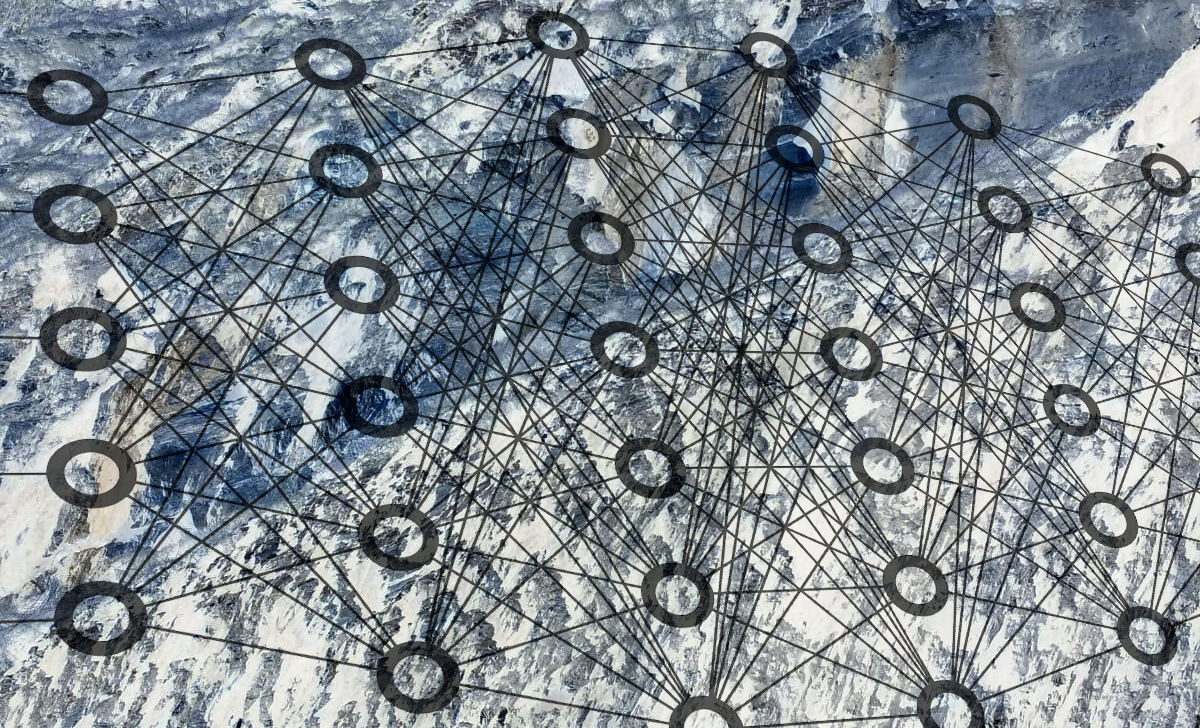
\includegraphics[height=\paperheight,width=\paperwidth]{frames/auxiliar/title_img/prueba.png}};}

\begin{frame}[plain]
\vspace{1cm}
\titlepage

\vspace{-0.2cm}

\includegraphics[height=0.2\textheight]{frames/auxiliar/title_img/upv_transparente.png} \hspace*{7.2cm}

\includegraphics[height=0.2\textheight]{frames/auxiliar/title_img/bcam_transparente.png} \hspace*{0.2cm}
\end{frame} 

}
%%%%%%%%%%%%%%%%%%%%%%%%%%%%%%%%%%
%%%%%%%%%%%%%%%%%%%%%%%%%%%%%%%%%%
%%%%%%%%%%%%%%%%%%%%%%%%%%%%%%%%%%
%\begin{section}{Geophysical Problems}
%\begin{frame}{Geophysical Applications: Earthquakes}

%\titlepage
\vspace{-0.4cm}
\center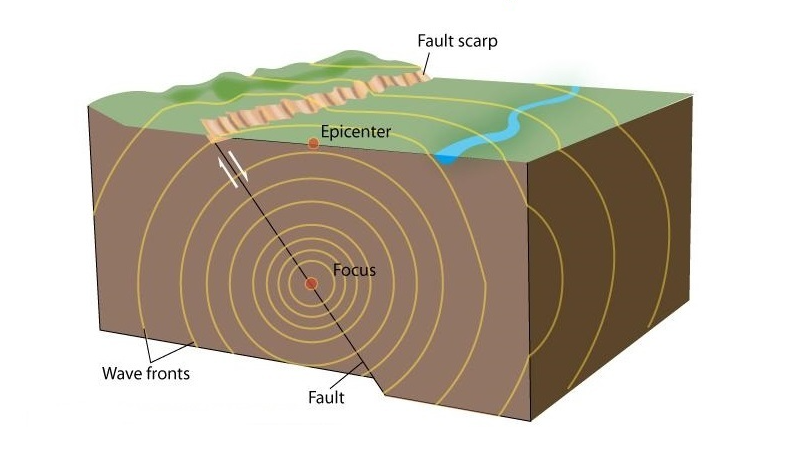
\includegraphics[height=4cm]{Diapos/Intro/Figures/natural_seismicity}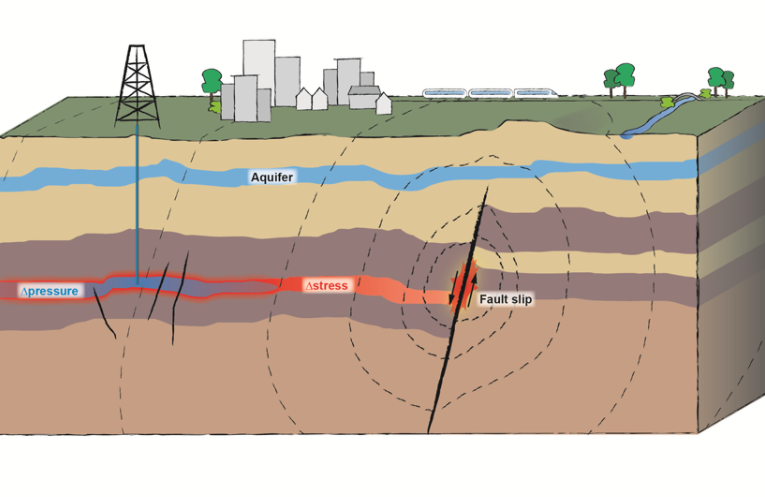
\includegraphics[height=4cm]{Diapos/Intro/Figures/induced_seismicity}\\

\vspace{-0.35cm}
\center\scriptsize{Natural seismicity  \textit{(Source: sciencelearn.org.nz)} and induced seismicity \textit{(Source: eos.org)}.}

\vspace{1cm}
\raggedright\normalsize{Knowing the hazard of each area is essential to estimate and prevent the effect of earthquakes.}
%\includegraphics[height=0.11\textheight]{./logos/logo_upv.jpg} \hspace*{0.2cm}
%includegraphics[height=0.11\textheight]{./logos/logo_bcam.jpg} \hspace*{0.2cm}
\end{frame} 

%%%%%%%%%%%%%%%%%%%%%%%%%%%%%%%%

\begin{frame}{Geophysical Applications: Energy  $\&$ Climate Change}

%\titlepage
\vspace{-0.2cm}
\center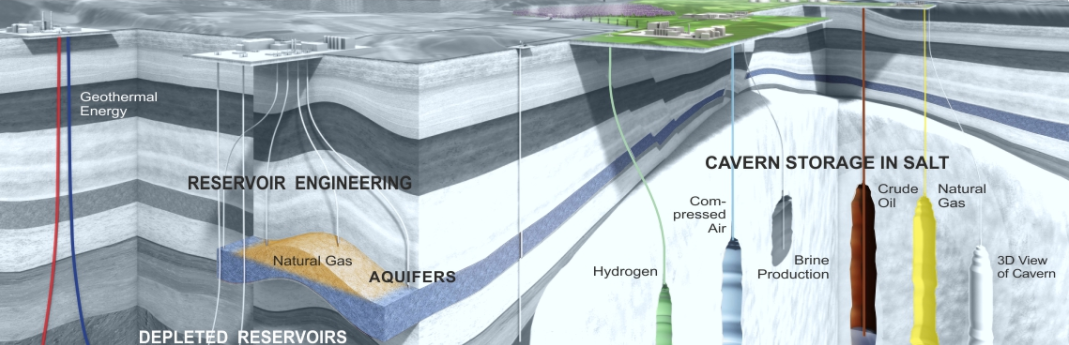
\includegraphics[height=4cm]{Diapos/Intro/Figures/Room_for_energy} \hspace*{0.2cm}\\
\vspace{-0.35cm}
\center\scriptsize{Source: https://deep-kbb.de/}

\vspace{1cm}
\raggedright\normalsize{\textbf{Geothermal energy, oil and gas exploitation, H$_2$  $\&$ CO$_2$ storage} require characterization and monitoring of the Earth's subsurface.}
%\includegraphics[height=0.11\textheight]{./logos/logo_upv.jpg} \hspace*{0.2cm}
%includegraphics[height=0.11\textheight]{./logos/logo_bcam.jpg} \hspace*{0.2cm}
\end{frame} 

%%%%%%%%%%%%%%%%%%%%%%%%%%%%%%%%

\begin{frame}{Exploration Method: Geosteering}

%\titlepage
\vspace{0.1cm}
\center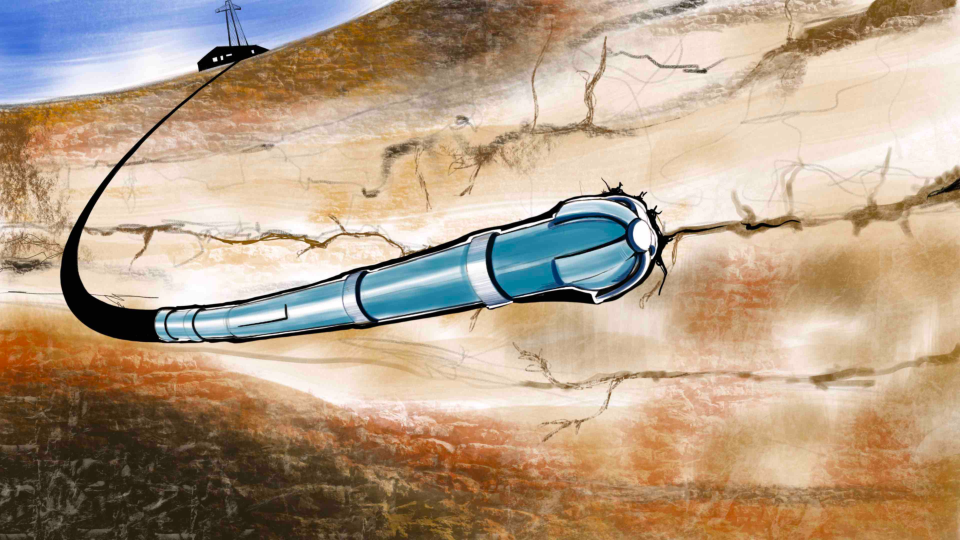
\includegraphics[height=3cm, width=10cm]{Diapos/Intro/Figures/Geosteering_drawing} \hspace*{0.2cm}\\
%\vspace{-0.35cm}
%\center\scriptsize{Source: https://deep-kbb.de/}

\vspace{0.4cm}
\raggedright\normalsize{\textbf{Geosteering.} The act of adjusting the borehole position in \textbf{real-time} to reach one or more targets.}

\visible<2>{
\begin{figure}
\centering
	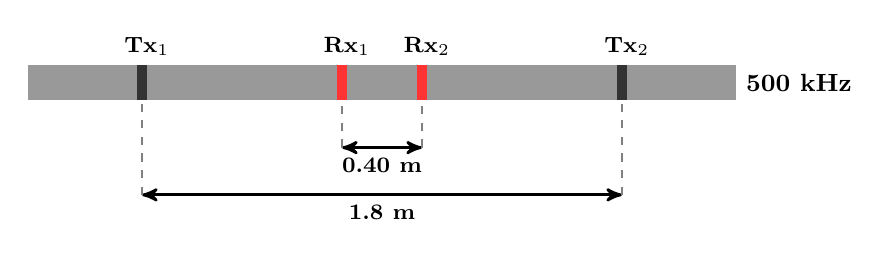
\begin{tikzpicture}

%% Tool
\fill[gray!80!white] (-1.5*3,0) -- (1.5*3,0.) --  node[right] {\small \bf \textcolor{black}{500 kHz}}  (1.5*3, 0.15*3) -- (-1.5*3,0.15*3) -- cycle;

%% Transmitters
\fill[black!80!white] (-0.6096*5-0.02*3,0) -- (-0.6096*5+0.02*3,0.) -- (-0.6096*5+0.02*3, 0.15*3) node[above] {\footnotesize \bf \textcolor{black}{Tx$_1$}}  -- (-0.6096*5-0.02*3,0.15*3) -- cycle;
%
\fill[black!80!white] (0.6096*5-0.02*3,0) -- (0.6096*5+0.02*3,0.)  -- (0.6096*5+0.02*3, 0.15*3) node[above] {\footnotesize \bf \textcolor{black}{Tx$_2$}} -- (0.6096*5-0.02*3,0.15*3) -- cycle;

%% Receivers
\fill[red!80!white] (-0.1016*5-0.02*3,0) -- (-0.1016*5+0.02*3,0.)  -- (-0.1016*5+0.02*3, 0.15*3) node[above] {\footnotesize \bf \textcolor{black}{Rx$_1$}} -- (-0.1016*5-0.02*3,0.15*3) -- cycle;
\fill[red!80!white] ( 0.1016*5-0.02*3,0) -- ( 0.1016*5+0.02*3,0.) -- ( 0.1016*5+0.02*3, 0.15*3)  node[above] {\footnotesize \bf \textcolor{black}{Rx$_2$}} -- ( 0.1016*5-0.02*3,0.15*3) -- cycle;

%% distances
\draw[black, line width=1pt,<->] (-0.1016*5, -0.6)      -- (0.1016*5, -0.6) node[pos=0.5, below] {\footnotesize \bf \textcolor{black}{0.40 m}}  ;
\draw[gray, dashed] (-0.1016*5, -0.6)      -- (-0.1016*5, 0)  ;
\draw[gray, dashed] ( 0.1016*5, -0.6)      -- ( 0.1016*5, 0)  ;

\draw[black, line width=1pt,<->] (-0.6096*5, -1.2)      -- (0.6096*5, -1.2) node[pos=0.5, below] {\footnotesize \bf \textcolor{black}{1.8 m}}  ;
\draw[gray, dashed] (-0.6096*5,-1.2)      -- (-0.6096*5, 0)  ;
\draw[gray, dashed] ( 0.6096*5,-1.2)      -- ( 0.6096*5, 0)  ;


\end{tikzpicture}
\end{figure}
}
\end{frame} 

%\begin{frame}{Governing PDEs in Geophysics}
\begin{columns}
\begin{column}{0.35\textwidth}
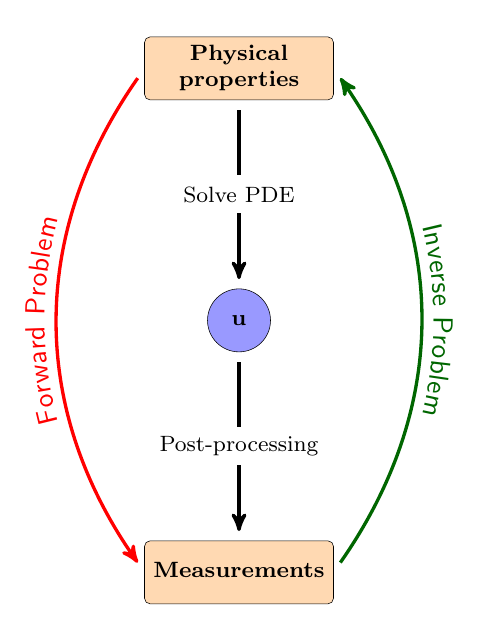
\begin{tikzpicture}[x=0.8cm, y=0.8cm]
%Material   Block A
\draw[very thin,rounded corners=2pt, fill=orange!30!white ] (-1.5,0) rectangle (1.5,1);
\node[color=black] at (0,0.5) {\footnotesize \textcolor{black}{\textbf{\begin{tabular}{c} Physical \\ properties \end{tabular}}}};
%Measurments Block C
\draw[very thin,rounded corners=2pt, fill=orange!30!white ] (-1.5,-8) rectangle (1.5,-7);
\node[color=black] at (0,-7.5) {\footnotesize \textcolor{black}{\textbf{\begin{tabular}{c} Measurements \end{tabular}}}};
%%PDE -- Block U
%\draw[very thin,rounded corners=2pt, fill=black ] (4.5,0) rectangle (5.5,1);
\draw[very thin, fill=blue!40!white] (0,-3.5) ellipse (0.5 and 0.5);
\node[color=black] at (0,-3.5) {\footnotesize \textcolor{black}{\textbf{\begin{tabular}{c} u \end{tabular}}}};
%
%%Define some nodes for origen-destination
\node (Aup) at (0,1) {};
\node (Adw) at (0,0) {};
\node (Ar) at (1.5,0.5) {};
\node (Al) at (-1.5,0.5) {};
%
\node (Cup) at (0,-7) {};
\node (Cdw) at (0,-8) {};
\node (Cr) at (1.5,-7.5) {};
\node (Cl) at (-1.5,-7.5) {};
%
\node (Uup) at (0,-3) {};
\node (Udw) at (0,-4) {};
%%arrows
\draw [<-,very thick, draw = green!40!black, postaction={decorate,decoration={raise=1ex,text along path,text align=center,text={|\color{green!40!black}\sffamily|Inverse Problem}}}] (Ar) to [bend left=35] (Cr);
%
\draw [<-,very thick, draw = red, postaction={decorate,decoration={raise=1ex,text along path,text align=center,text={|\color{red}\sffamily|Forward Problem}}}] (Cl) to [bend left=35] (Al);
%
\draw [<-,draw = black, very thick,] (Uup) to [bend left=0]  (Adw);
%
\draw [<-,draw = black, very thick, ] (Cup) to [bend left=0]  (Udw);
%
\fill[fill=white] (-1.5,-5.2) rectangle (1.5,-5.8);
\node at (0,-5.5) {\footnotesize Post-processing};
\fill[fill=white] (-1.5,-1.2) rectangle (1.5,-1.8);
\node at (0,-1.5) {\footnotesize Solve PDE};
\end{tikzpicture}
\end{column}
%
\begin{column}{0.55\textwidth}
{\large Maxwell's equations}
\vspace{0,15cm}
\begin{equation}
\notag
\left\{
                \begin{array}{lll}
                \vspace{0,2cm}
                  \mathbf{\nabla} \times \mathbf{H} & = (\boldsymbol{\sigma} + j \omega \boldsymbol{\epsilon})\mathbf{E} + \mathbf{J}^{imp} & \textup{Ampère's law,}\\
                  \vspace{0,2cm}
                  \mathbf{\nabla} \times \mathbf{E} & = -j \omega \boldsymbol{\mu}\mathbf{H} + \mathbf{M}^{imp} & \textup{Faraday's law,}\\
                  \mathbf{\nabla} \cdot (\boldsymbol{\epsilon}\mathbf{E}) & = \rho_{e} & \textup{Gauss' law of} \\
                  \vspace{0,2cm}
                  & & \textup{electricity,} \\
                  \mathbf{\nabla} \cdot (\boldsymbol{\mu}\mathbf{H}) & =0 & \textup{Gauss' law of} \\
                 & & \textup{magnetism.}
                \end{array}
              \right.
\end{equation}
\end{column}
\end{columns}
\end{frame}



%\begin{frame}{Traditional Numerical Methods in Geophysics}
  \begin{columns}[T,onlytextwidth]
  
    \begin{column}{0.48\textwidth}
      \begin{figure}
        \centering % This ensures the image is centered in the column
        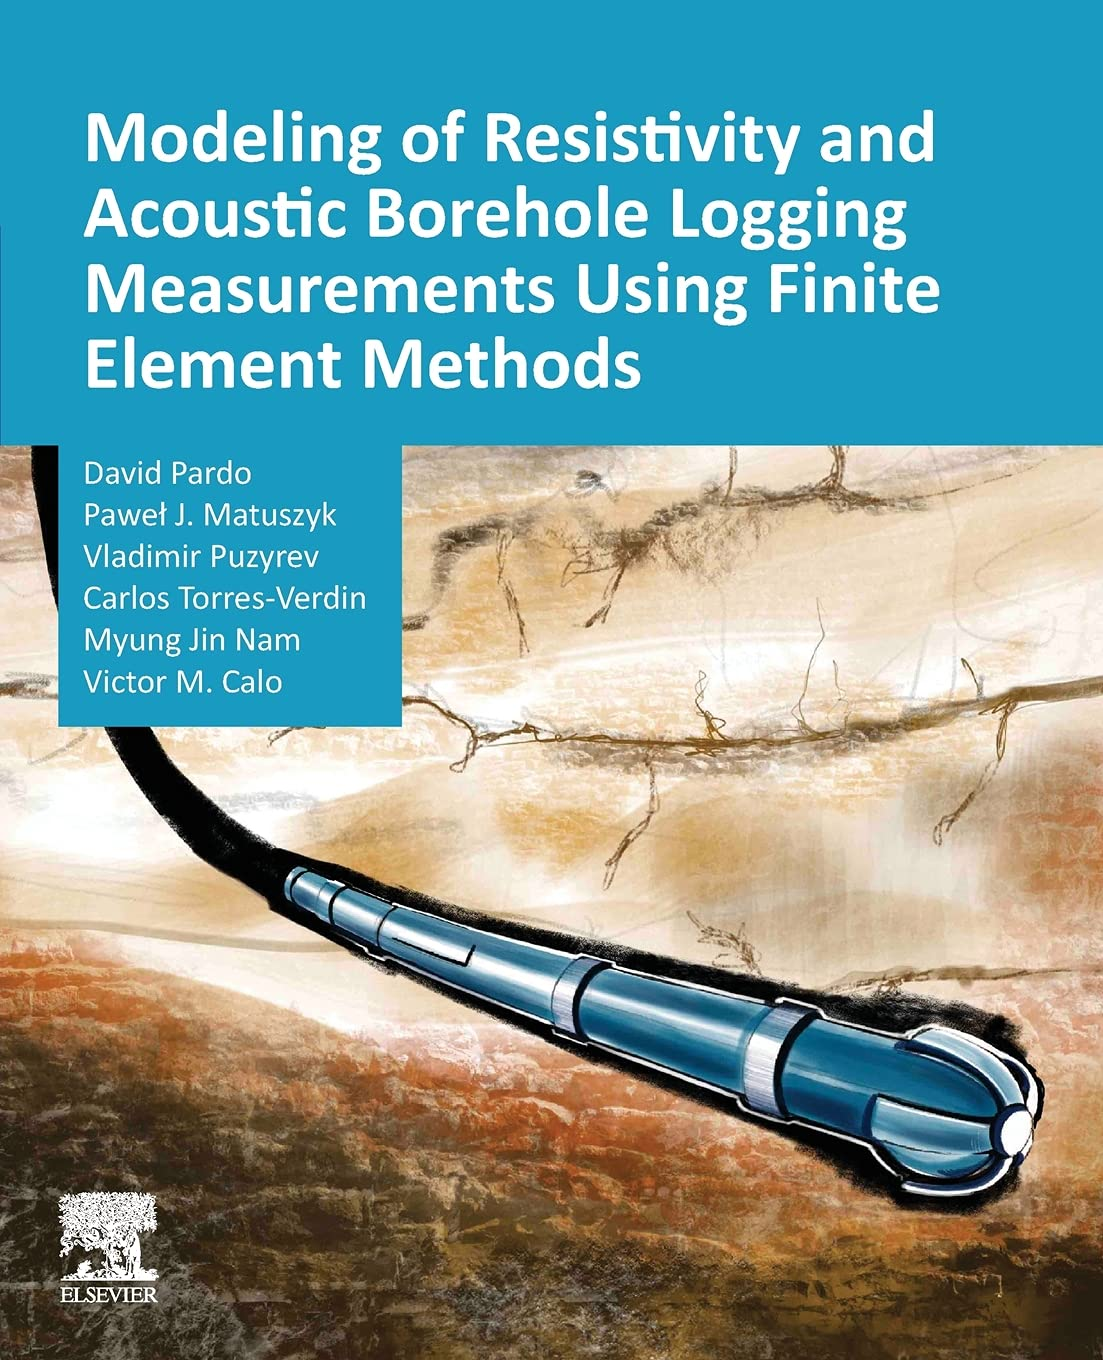
\includegraphics[width=0.8\textwidth]{Diapos/Intro/Figures/PardoBook.jpg} % Using width=\textwidth instead of scale
        \caption{Published in 2021} % Optional caption for the figure
        \label{fig:book} % Label for referencing the figure if needed
      \end{figure}
    \end{column}
    
    \begin{column}{0.48\textwidth}
      \begin{block}{Numerical Methods}
        \begin{itemize}
          \setlength\itemsep{2.4em} % Adjust the space between items
          \item Finite Element method
          \item Finite Difference method
          \item Finite Volumes method
          \item Integral methods
          \item Semi-analytical methods
        \end{itemize}
      \end{block}
    \end{column}
    
  \end{columns}
\end{frame}

%\end{section}
%%%%%%%%%%%%%%%%%%%%%%%%%%%%%%%%%%
%{
\usebackgroundtemplate{\tikz\node[opacity=0.07,inner sep=0] {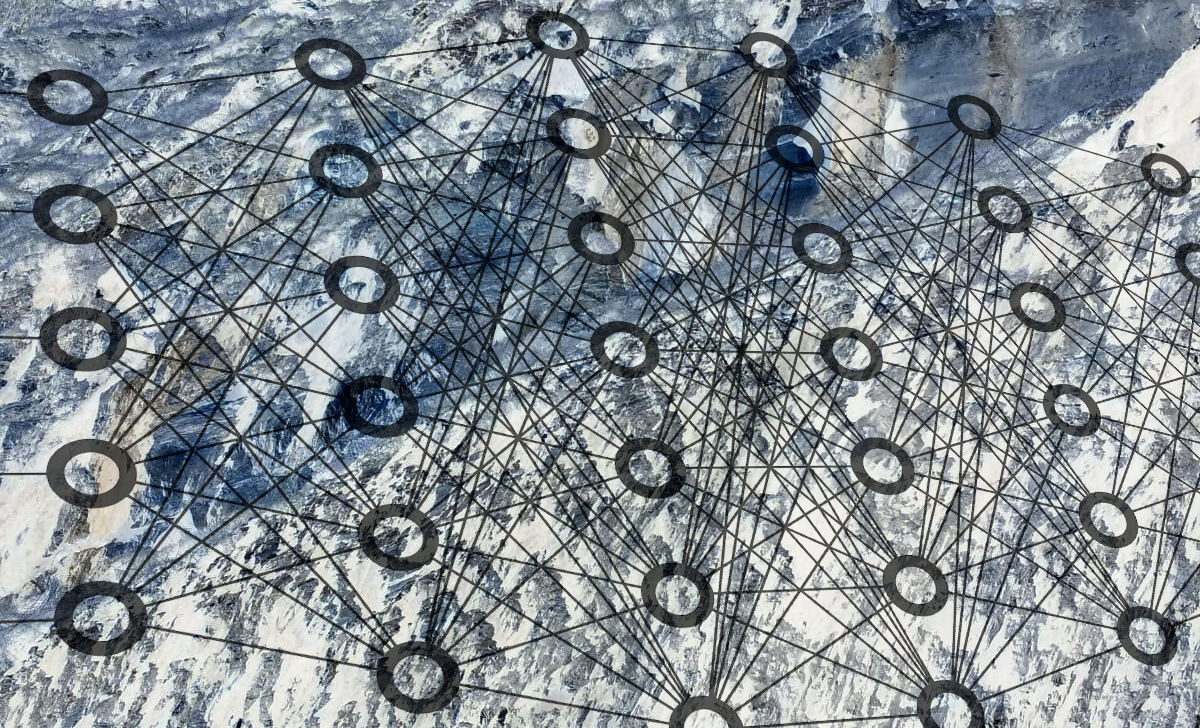
\includegraphics[height=\paperheight,width=\paperwidth]{frames/auxiliar/title_img/prueba.png}};}

\begin{frame}{Outline}
\begin{columns}
\begin{column}{0.05\textwidth}
\end{column}
\begin{column}{0.95\textwidth}

\mybullet{1}{Why Use Deep Learning?}

\vspace{0.4cm}

\mybullet{2}{Deep Learning for Solving Inverse and Forward Problems}

\vspace{0.4cm}

\mybullet{3}{Database Generation using rIGA}
%	\vspace{-0.2cm}
%	\begin{itemize}\setlength{\itemindent}{1cm}
%	\item Existing methods
%	\item Limitation for geophysical problems
%	\item Challenges: Integration, and Minimization
%	\end{itemize}

\vspace{0.4cm}

\mybullet{4}{Solving Forward Problems (PDEs) with Neural Networks}
%	\vspace{-0.2cm}
%	\begin{itemize}\setlength{\itemindent}{1cm}
%	\item Deep Finite Element Method
%	\item $r-$adaptivity with Deep Learning
%	\item Building the Riesz Operator with Deep Methods
%	\item Deep Fourier Method
%\end{itemize}


\vspace{0.4cm}

\mybullet{5}{Achievements}

\vspace{0.4cm}

\mybullet{6}{Conclusions and Future Work}
\end{column}
\end{columns}

\end{frame} 
}
%%%%%%%%%%%%%%%%%%%%%%%%%%%%%%%%%%
%\begin{section}{Why use Deep Learning for Geophysics?}
%{
\usebackgroundtemplate{\tikz\node[opacity=0.1,inner sep=0] {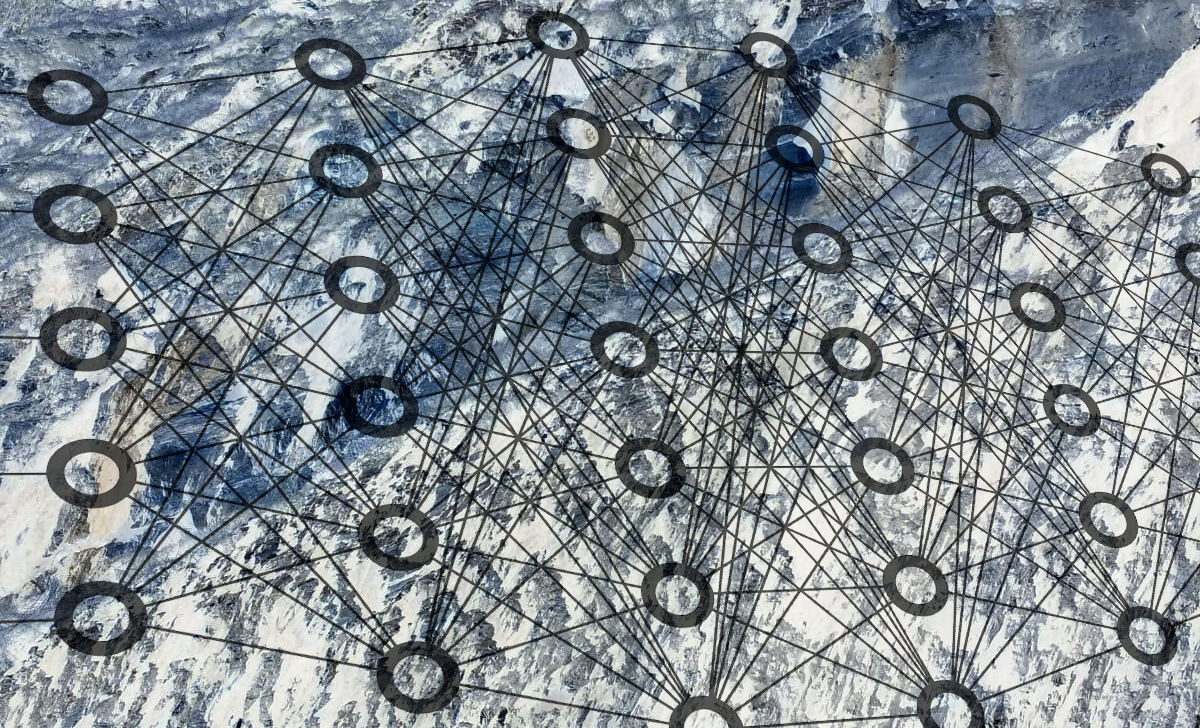
\includegraphics[height=\paperheight,width=\paperwidth]{frames/auxiliar/title_img/prueba.png}};}
%%%%%%%%
\begin{frame}[plain]
\begin{variableblock}{}{bg=myblue,fg=white}{bg=green,fg=red}
\begin{center}
\textbf{Why use Deep Learning for Geophysics?}
\end{center}
\end{variableblock}
\end{frame}
%%%%%%%%%%%%%%%%%%%%%%%%%%%%%%%%%%%%%%%%%%%%%%%%%%%%%%%%%%%%%%%%%%%
}
%\def\layersep{1.5cm}

\begin{frame}{What is Deep Learning?}
\begin{minipage}[t]{0.48\linewidth}
\vspace{-0.1cm}
\begin{figure}
	\hspace{-1cm}
	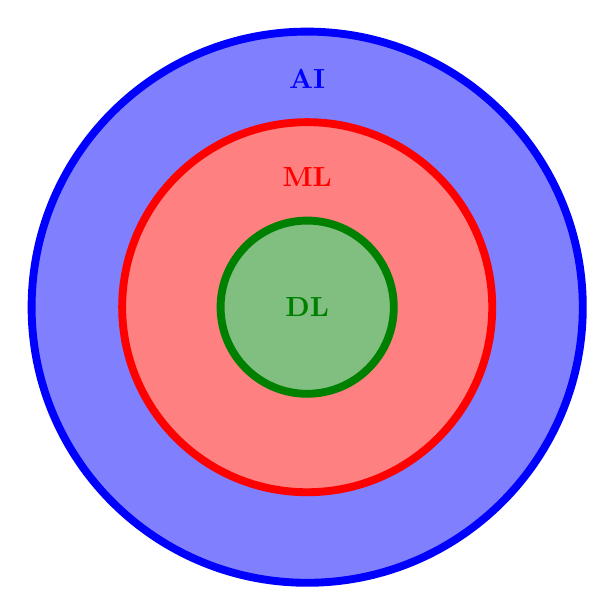
\begin{tikzpicture}[x=1cm, y=1cm, line width=1mm]
    \visible<3-3>{\path [draw=blue,fill=blue!50] (0,0) circle (3.55cm-0.5\pgflinewidth);}
    \visible<2-3>{\path [draw=red,fill=red!50] (0,0) circle (2.4cm-0.5\pgflinewidth);}
    \visible<1-3>{\path [draw=jon_green,fill=jon_green!50,line width=1mm] (0,0) circle (1.15cm-0.5\pgflinewidth);}
    \visible<1-3>{\node[jon_green] at (0,0) {\textbf{DL}};}
    \visible<2-3>{\node[red] at (0,1.65) {\textbf{ML}};}
    \visible<3-3>{\node[blue] at (0,2.9) {\textbf{AI}};}
\end{tikzpicture}
\end{figure}
\end{minipage}
\begin{minipage}[t]{0.48\linewidth}
\visible<1-3>{\textcolor{jon_green}{Deep Learning (DL)} is part of a broader family of \textcolor{red}{Machine Learning (ML)} methods based on artificial Neural Networks. \textit{Wikipedia}}
\vspace{0.2cm}

\visible<2-3>{\textcolor{red}{Machine learning (ML)} is seen as a part of \textcolor{blue}{Artificial Intelligence (AI)} that is devoted to understanding and building methods that \textit{learn}. \textit{Wikipedia}}
\vspace{0.2cm}

\visible<3-3>{\textcolor{blue}{Artificial Intelligence (AI)} is the theory and development of computer systems able to perform tasks that normally require human intelligence, such as visual perception, speech recognition, or decision-making. \textit{Oxford English Dictionary}}
\end{minipage}
\end{frame}


\begin{frame}{Deep Learning Methods}
\textbf{Advantages:}
\vspace{0.4cm}
\begin{itemize}
\item Affordable computational cost (\textit{High offline, low online})
\vspace{0.4cm}
\item Easily parallelizable implementation
\vspace{0.4cm}
\item Great approximation capabilities
\vspace{0.4cm}
\item Exploitable big data
\vspace{0.4cm}
\item Constant advances in computers
\vspace{0.4cm}
\item Trendy among the scientific community
\end{itemize}
\end{frame}


\begin{frame}[t]{Deep Learning Working Areas}
Language Processing
\begin{thebibliography}{1}
\bibitem{DL_lp} \small{D. Otter, J. Medina, and J. Kalita. A Survey of the Usages of Deep Learning for Natural Language Processing. IEEE Transactions on Neural Networks and Learning Systems, 32(2): 604-624, 2021.}
\end{thebibliography}
%https://ieeexplore.ieee.org/abstract/document/9075398?casa_token=un977of__0gAAAAA:f7OQhF6nUr9fNvTePPyrNz2_6Id2GxED9oyu6jtgdhnsaZxykeKdZHdvXJcNp6d0MBlqeY__
\vspace{0.5cm}

Image Processing
\begin{thebibliography}{2}
\bibitem{DL_image} \small{M. Egmont-Petersen, D. de Ridder, and H. Handels. Image processing with neural networks—a review. Pattern Recognition, 35(10): 2279-2301, 2002.}
\end{thebibliography}
%https://www.sciencedirect.com/science/article/abs/pii/S0031320301001789
\vspace{0.5cm}

Healthcare
\begin{thebibliography}{3}
\bibitem{DL_health} \small{A. Esteva et al. A guide to deep learning in healthcare. Nature Medicine, 25: 24–29, 2019.}
\end{thebibliography}
%https://www.nature.com/articles/s41591-018-0316-z?source=post_page---------------------------
\end{frame}


%\begin{frame}[t]{Artificial Neural Networks}
%\visible<1-2>{Artificial neural networks (also known in literature as Neural Networks) are computing systems inspired by the biological neural networks.}
%\vspace{0.3cm}
%
%They are composed of connected units called artificial neurons or nodes. 
%
%\vspace{0.3cm}
%\visible<2>{A node receives signals, then processes them and send the information to neurons connected to it.}
%
%\only<2>{
%\begin{figure}
%	\hspace{-2cm}
%	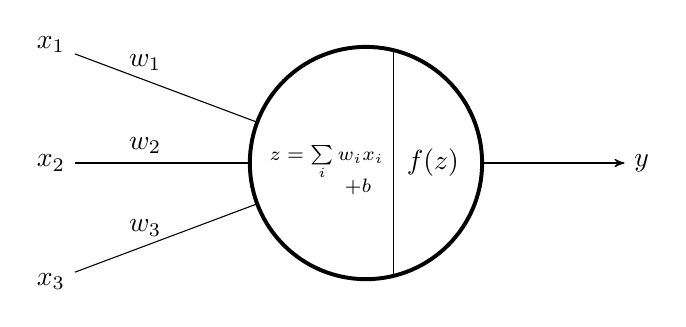
\begin{tikzpicture}
    \node[] at (-4,1.5) (a1) {\textbf{$x_1$}};
    \node[] at (-4,0) (a2) {\textbf{$x_2$}};
    \node[] at (-4,-1.5) (a3) {\textbf{$x_3$}};
    
    \node[] at (0,0) (b) {};
    
    \node[] at (3.5,0) (c) {\textbf{$y$}};  
    
	\path[->] (a1) edge node [near start,above] {$w_1$} (b);
	\path[->] (a2) edge node [near start,above] {$w_2$} (b);
	\path[->] (a3) edge node [near start,above] {$w_3$} (b);
    
    \path[->] (b) edge node [near start,above] {} (c);
    
    \path [draw=black,fill=white,line width=0.5mm] (0,0) circle (1.5cm-0.5\pgflinewidth);
    
%    \node[] at (-0.5,0.6) (b1) {$z$};
%	\node[rotate=90] at (-0.5,0.3) (b1) {$=$};
    \node[] at (-0.5,0) (b1) {{\scriptsize $z=\sum\limits_{i} w_i x_i$}};
    \node[] at (-0.1,-0.3) (b2) {{\scriptsize $ + b$}};
    
    \node[] at (0.35,1.57) (d1) {};
    \node[] at (0.35,-1.57) (d2) {};
    \path[] (d1) edge node [near start,above] {} (d2);
	\node[] at (0.85,0) (b3) {$f(z)$};
\end{tikzpicture}
%\end{figure}
%}
%\end{frame}


\begin{frame}[t]{Artificial Neural Networks}\linespread{1.05}
\vspace{-.2 cm}
\begin{center}
	Approximate: ${\cal I} \approx {\cal I}_{\phi} := A_k \circ N \circ A_{k-1}  \circ \cdots \circ N \circ A_1 $\\
\end{center}
\only<1-2>{
	\vspace{0.2 cm}
	\centerline{$N$ -- Non-linear activation function  \hspace{0.3 cm};\hspace{0.3 cm} $A_k$ -- Affine transformation}
	\vspace{0.6cm}
\begin{figure}
	\vspace*{-0.25in}
	\begin{tikzpicture}
	\visible<2>{
	\node[] () at (0,-0.2) {\begin{tikzpicture}[scale=0.62]
		\begin{axis}[
		%ticks=none,
		height=0.5\textwidth,
		width=0.1\textwidth,
		scale only axis,
		enlargelimits=false,
		axis on top,
		xlabel={Resistivity [$\Omega$m]},
		xtick={0,1.2,2.39},
		xticklabels={100,200,300},
		ytick={0.93,1.85,2.78,3.7,4.65,5.56,6.50,7.44,8.37,9.305,10.24,11.18,12.08,13},
		yticklabels={130,120,110,100,90,80,70,60,50,40,30,20,10,0},
		ylabel={Deep [m]},
		label style={font=\tiny},
		tick label style={font=\tiny}] 
		\addplot[thick] graphics[xmin=0,xmax=3,ymin=0,ymax=13] {Diapos/Intro/Figures/resis1};
		\end{axis}
		\end{tikzpicture}};
		}
		
	\node[] () at (4.3,0.2) {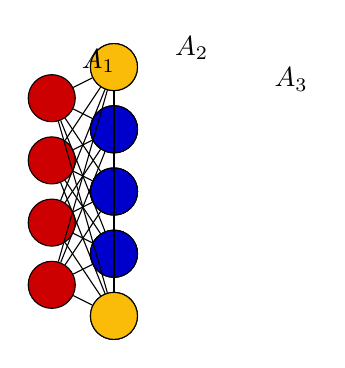
\begin{tikzpicture}[scale=0.79]
		\tikzstyle{every pin edge}=[<-,shorten <=1pt]
		\tikzstyle{neuron}=[circle,fill=black!25,minimum size=17pt,inner sep=0pt]
		\tikzstyle{input neuron}=[neuron,draw=black,fill=red!80!black];
		\tikzstyle{output neuron}=[neuron,draw=black,fill=blue!80!black];
		\tikzstyle{hidden neuron}=[neuron,draw=black,fill=yellow!50!orange];
		\tikzstyle{annot} = [text width=4em, text centered]
			
			% Draw the input layer nodes
		\foreach \name / \y in {1,...,4}
		% This is the same as writing \foreach \name / \y in {1/1,2/2,3/3,4/4}
		\node[input neuron] (I-\name) at (0,-\y) {};
			
			% Draw the hidden layer nodes
		\foreach \name / \y in {1,...,5}
		\path[yshift=0.5cm]
		node[hidden neuron] (H-\name) at (\layersep,-\y cm) {};
			
			% Draw the hidden layer nodes
		\foreach \name / \y in {1,...,5}
		\path[yshift=0.5cm]
		node[hidden neuron] (H2-\name) at (\layersep+\layersep,-\y cm) {};
			
			
			% Draw the output layer node
		\foreach \name / \y in {1,...,3}
		\path[yshift=-0.5cm]
		node[output neuron] (O-\name) at (\layersep+\layersep+\layersep,-\y cm) {};
			
			% Connect every node in the input layer with every node in the
			% hidden layer.
		\foreach \source in {1,...,4}
		\foreach \dest in {1,...,5}
		\path (I-\source) edge (H-\dest);
			
		\foreach \source in {1,...,5}
		\foreach \dest in {1,...,5}
		\path (H-\source) edge (H2-\dest);
			
			% Connect every node in the hidden layer with the output layer
		\foreach \source in {1,...,5}
		\foreach \dest in {1,...,3}
		\path (H2-\source) edge (O-\dest);

	    \node[] () at (0.75, -.4) {$A_1$};	
		\node[] () at (2.25, -0.2) {$A_2$};
		\node[] () at (3.85,-.7) {$A_3$};
			% Annotate the layers
		\end{tikzpicture}};
	\node[] () at (4.3, 2.8) {Neural Network};		
	\visible<2>{	
	\node[] () at (8.8, 1.2) {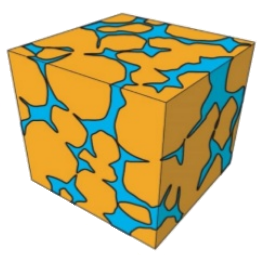
\includegraphics[width=2.5cm]{Diapos/Intro/Figures/res1}};
	\node[] () at (8.8,-1.4) {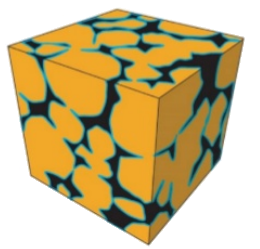
\includegraphics[width=2.5cm]{Diapos/Intro/Figures/res2}};
	\node[] () at (8.4, 2.8) {Output};
	\node[] () at (0.2, 2.8) {Input};
		
	\draw [decorate,very thick,decoration={brace,amplitude=10pt},xshift=-4pt,yshift=0pt]
		(1.3,2.8) -- (1.3,-2.4);
	\draw [decorate,very thick,decoration={brace,amplitude=10pt},xshift=-4pt,yshift=0pt]
		(7.5,-2.4) -- (7.5,2.8);
		
	\node[right] () at (9.0, 0.0) {\scriptsize Water};		
	\node[right] () at (9.0, -2.5) {\scriptsize Oil};	
	}			
\end{tikzpicture}
\end{figure}}
\only<3>{
	\vspace{0.4cm}
	
	$A_k$ -- Affine transformation: \hspace{0.1cm} $A_k \cdot x+b_k$
	\vspace{0.4cm}
	
	$N$ -- Non-linear activation function:

	\begin{figure}
	\centering
		\begin{subfigure}{.5\textwidth}
		\centering
		\begin{tikzpicture}[scale=0.7]
\begin{axis}[
    xmin=-2.5, xmax=2.5,
    ymin=-1.5, ymax=1.5,
    axis lines=center,
    axis on top=true,
    domain=-2.5:2.5,
    ylabel=$tanh(x)$,
    xlabel=$x$,
    x label style={at={(axis description cs:0.5,-0.1)},anchor=north},
    y label style={at={(axis description cs:-0.1,.5)},rotate=90,anchor=south},
    ]

    \addplot [mark=none,draw=blue,ultra thick] {tanh(\x)};
%    \node [right, red] at (axis cs: 1,0.7) {$y = \tanh x$};
    
    %% Add the asymptotes
%    \draw [blue, dotted, thick] (axis cs:-2.5,-1)-- (axis cs:0,-1);
%    \draw [blue, dotted, thick] (axis cs:+2.5,+1)-- (axis cs:0,+1);
\end{axis}
\end{tikzpicture}

		%	\caption{Tanh}
		\label{fig:tanh}
		\end{subfigure}%
		\begin{subfigure}{.5\textwidth}
		\centering
		\begin{tikzpicture}[scale=0.7,
  declare function={
    func(\x)= (\x < 0) * (0)   +
                   + (\x >= 0) * (\x);
  }
]
\begin{axis}[
    xmin=-2.5, xmax=2.5,
    ymin=-1.5, ymax=1.5,
    axis lines=center,
    axis on top=true,
    domain=-2.5:2.5,
  ylabel=$ReLU(x)$,
  xlabel=$x$,
     x label style={at={(axis description cs:0.5,-0.1)},anchor=north},
    y label style={at={(axis description cs:-0.1,.5)},rotate=90,anchor=south}, % added
]

\addplot [blue,ultra thick] {func(x)};
\end{axis}
\end{tikzpicture} 
		%	\caption{Tanh}
		\label{fig:tanh}
		\end{subfigure}
%	\caption{A figure with two subfigures}
	\label{fig:test}
	\end{figure}
	}
\end{frame}


\begin{frame}[t]{Deep Learning in Geophysics}
%They train a CNN to approximate the inverse operator. They use different metrics to control the value of the loss and use dropout method as regularization. 
%\begin{thebibliography}{4}
%\bibitem{geo_1} \small{D. Moghadas. One-dimensional deep learning inversion of electromagnetic induction data using convolutional neural network. Geophysical Journal International, 222(1): 247-259, 2020.}
%\end{thebibliography}
%https://academic.oup.com/gji/article-abstract/222/1/247/5818323
They train a CNN to approximate the inverse operator. They use the data misfit loss function with MSE metric and add a regularization term.
\begin{thebibliography}{5}
\bibitem{geo_2} \small{B. Liu et al. Deep Learning Inversion of Electrical Resistivity Data. IEEE Transactions on Geoscience and Remote Sensing, 58(8): 5715-5728, 2020.}
\end{thebibliography}
\vspace{0.2cm}

The model outputs several likely inverse solutions and it also predicts their probabilities. 
\begin{thebibliography}{5}
\bibitem{geo_2} \small{ S. Alyaev and A. H. Elsheikh. Direct multi-modal inversion of geophysical logs using deep learning. Earth and Space Science, 9, e2021EA002186, 2022.}
\end{thebibliography}
%https://ieeexplore.ieee.org/abstract/document/8994191?casa_token=dBQ0UUmOSyUAAAAA:vre7sUUy3QZ6OyaCxwigpHbmfR-HZdQWcXJ-Z0YMwDyMWXFnPISVJuEJlslqWLvuSZ1pvHa-iGvy
\vspace{0.2cm}

%En este utiliza un loss normal, el missfit, pero parte de una solucion a priori (o puede ser random tambien). Ellos no entrenan el inverso aqui, lo evaluan en el loss.
%\begin{thebibliography}{6}
%\bibitem{geo_3} \small{Y. Shi, X. Wu, and S. Fomel. Deep learning parameterization for geophysical inverse problems. SEG Global Meeting Abstracts, 36-40, 2020.}
%\end{thebibliography}
%%https://library.seg.org/doi/abs/10.1190/iwmg2019_09.1

\visible<2>{In the first part of this dissertation, \textbf{we analyze the behavior of different loss functions while solving inverse problems using Deep Learning.}
\begin{thebibliography}{6}
\bibitem{DL_me} \small{M. Shahriari, D. Pardo, J. A. Rivera et al. Error control and loss functions for the deep learning inversion of borehole resistivity measurements. International Journal for Numerical Methods in Engineering, 122(6): 1629-1657, 2021.}
\end{thebibliography}}
\end{frame}
%%\begin{frame}{Deep Learning Methods}
\textbf{Advantages:}
\vspace{0.4cm}
\begin{itemize}
\item Affordable computational cost (\textit{High offline, low online})
\vspace{0.4cm}
\item Easily parallelizable implementation
\vspace{0.4cm}
\item Great approximation capabilities
\vspace{0.4cm}
\item Exploitable big data
\vspace{0.4cm}
\item Constant advances in computers
\vspace{0.4cm}
\item Trendy among the scientific community
\end{itemize}
\end{frame}


\begin{frame}{LITERATURE REVIEW}
LITERATURE REVIEW.

porqué lo que tú has hecho ha sido una contribución dentro de los trabajos que existen.
\end{frame}
%\end{section}
%%%%%%%%%%%%%%%%%%%%%%%%%%%%%%%%%%
%%%%%%%%%%%%%%%%%%%%%%%%%%%%%%%%%%
%\begin{section}{Deep Learning for Solving Inverse and Forward Problems}x
%%%%%%%%%
{
\usebackgroundtemplate{\tikz\node[opacity=0.1,inner sep=0] {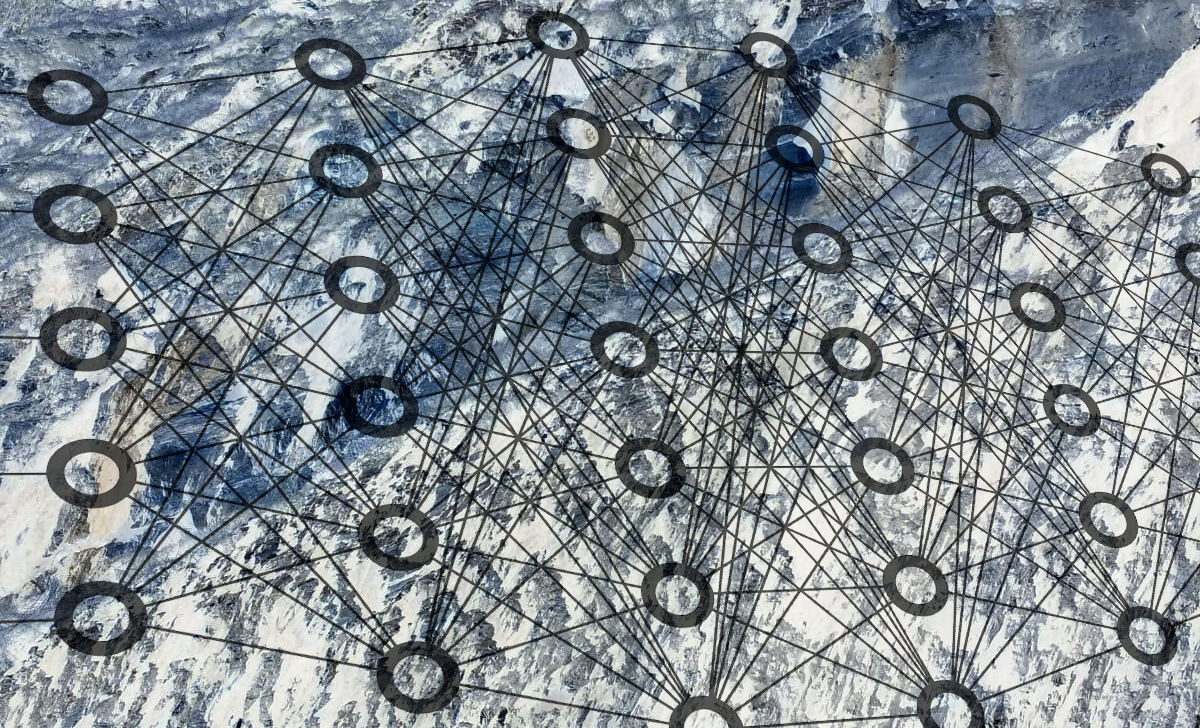
\includegraphics[height=\paperheight,width=\paperwidth]{frames/auxiliar/title_img/prueba.png}};}

\begin{frame}[plain]
\begin{variableblock}{}{bg=myblue,fg=white}{bg=green,fg=red}
\begin{center}
\textbf{Deep Learning for Solving Inverse (and Forward) Problems}
\end{center}
\end{variableblock}
\end{frame}
}
%%%%%%%%%%%%%%%%%%%%%%%%%%%%%%%%%%%%%%%%%%%%%%%%%%%%%%%%%%%%%%%%%%%
%\begin{frame}{Governing PDEs in Geophysics}
\begin{columns}
\begin{column}{0.35\textwidth}
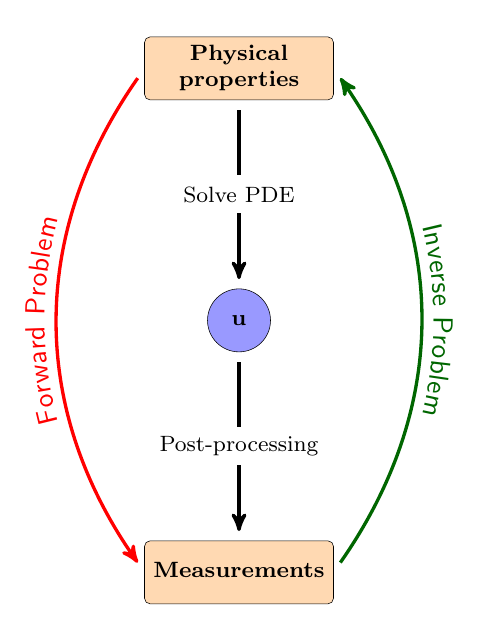
\begin{tikzpicture}[x=0.8cm, y=0.8cm]
%Material   Block A
\draw[very thin,rounded corners=2pt, fill=orange!30!white ] (-1.5,0) rectangle (1.5,1);
\node[color=black] at (0,0.5) {\footnotesize \textcolor{black}{\textbf{\begin{tabular}{c} Physical \\ properties \end{tabular}}}};
%Measurments Block C
\draw[very thin,rounded corners=2pt, fill=orange!30!white ] (-1.5,-8) rectangle (1.5,-7);
\node[color=black] at (0,-7.5) {\footnotesize \textcolor{black}{\textbf{\begin{tabular}{c} Measurements \end{tabular}}}};
%%PDE -- Block U
%\draw[very thin,rounded corners=2pt, fill=black ] (4.5,0) rectangle (5.5,1);
\draw[very thin, fill=blue!40!white] (0,-3.5) ellipse (0.5 and 0.5);
\node[color=black] at (0,-3.5) {\footnotesize \textcolor{black}{\textbf{\begin{tabular}{c} u \end{tabular}}}};
%
%%Define some nodes for origen-destination
\node (Aup) at (0,1) {};
\node (Adw) at (0,0) {};
\node (Ar) at (1.5,0.5) {};
\node (Al) at (-1.5,0.5) {};
%
\node (Cup) at (0,-7) {};
\node (Cdw) at (0,-8) {};
\node (Cr) at (1.5,-7.5) {};
\node (Cl) at (-1.5,-7.5) {};
%
\node (Uup) at (0,-3) {};
\node (Udw) at (0,-4) {};
%%arrows
\draw [<-,very thick, draw = green!40!black, postaction={decorate,decoration={raise=1ex,text along path,text align=center,text={|\color{green!40!black}\sffamily|Inverse Problem}}}] (Ar) to [bend left=35] (Cr);
%
\draw [<-,very thick, draw = red, postaction={decorate,decoration={raise=1ex,text along path,text align=center,text={|\color{red}\sffamily|Forward Problem}}}] (Cl) to [bend left=35] (Al);
%
\draw [<-,draw = black, very thick,] (Uup) to [bend left=0]  (Adw);
%
\draw [<-,draw = black, very thick, ] (Cup) to [bend left=0]  (Udw);
%
\fill[fill=white] (-1.5,-5.2) rectangle (1.5,-5.8);
\node at (0,-5.5) {\footnotesize Post-processing};
\fill[fill=white] (-1.5,-1.2) rectangle (1.5,-1.8);
\node at (0,-1.5) {\footnotesize Solve PDE};
\end{tikzpicture}
\end{column}
%
\begin{column}{0.55\textwidth}
{\large Maxwell's equations}
\vspace{0,15cm}
\begin{equation}
\notag
\left\{
                \begin{array}{lll}
                \vspace{0,2cm}
                  \mathbf{\nabla} \times \mathbf{H} & = (\boldsymbol{\sigma} + j \omega \boldsymbol{\epsilon})\mathbf{E} + \mathbf{J}^{imp} & \textup{Ampère's law,}\\
                  \vspace{0,2cm}
                  \mathbf{\nabla} \times \mathbf{E} & = -j \omega \boldsymbol{\mu}\mathbf{H} + \mathbf{M}^{imp} & \textup{Faraday's law,}\\
                  \mathbf{\nabla} \cdot (\boldsymbol{\epsilon}\mathbf{E}) & = \rho_{e} & \textup{Gauss' law of} \\
                  \vspace{0,2cm}
                  & & \textup{electricity,} \\
                  \mathbf{\nabla} \cdot (\boldsymbol{\mu}\mathbf{H}) & =0 & \textup{Gauss' law of} \\
                 & & \textup{magnetism.}
                \end{array}
              \right.
\end{equation}
\end{column}
\end{columns}
\end{frame}



%\begin{frame}{Key Concept}
\centerline{Different earth models may deliver identical measurements}
\vspace{0.2in}
\hspace{0.57in}
	\begin{tikzpicture}	
	\node at (2.0,0.0)[scale=1.03]{\begin{tikzpicture}[scale=1.5,
mipunto/.style ={color=red}]
\draw[fill=blue!70!brown] (-1.5,-1) -- (-1.5,0) -- (1.5,0) -- (1.5,-1) -- cycle;
\draw[fill=white!30!brown] (-1.5,1) -- (-1.5,0) -- (1.5,0) -- (1.5,1) -- cycle;
%\draw[line width=1.25mm,red] (0.0,0.0) -- (0.3,0.0);
\filldraw[mipunto] (0,0) circle (2.5pt);
\node (a) at (-1.,0.5) {$\rho_{1}$};  
\node (b) at (-1.,-0.5) {\textcolor{white}{$\rho_{2}$}};
\end{tikzpicture}
};
	\node at (9.0,0.0)[scale=1.03]{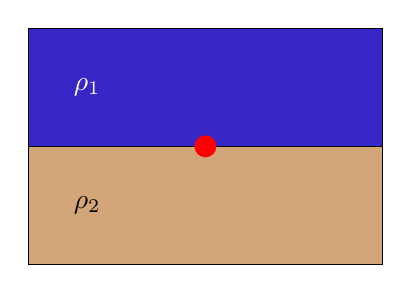
\begin{tikzpicture}[scale=1.5,
mipunto/.style ={color=red}]
\draw[fill=white!30!brown] (-1.5,-1) -- (-1.5,0) -- (1.5,0) -- (1.5,-1) -- cycle;
\draw[fill=blue!70!brown] (-1.5,1) -- (-1.5,0) -- (1.5,0) -- (1.5,1) -- cycle;
%\draw[line width=1.25mm,red] (0.0,0.0) -- (0.3,0.0);
\filldraw[mipunto] (0,0) circle (2.5pt);
\node (a) at (-1.,0.5) {\textcolor{white}{$\rho_{1}$}};  
\node (b) at (-1.,-0.5) {$\rho_{2}$};
\end{tikzpicture}
};
	\end{tikzpicture}
\end{frame}

\begin{frame}{Simple example}
\centering
Simple example of an inverse problem.\\
$\qquad$\\
\begin{figure}[!htp]
	\subcaptionbox{Forward function}{%
	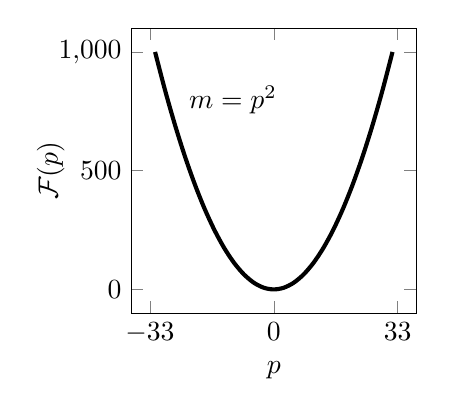
\begin{tikzpicture}
\begin{axis}
[scatter/classes={ a={mark=o,draw=blue}}, xlabel=$p$, ylabel=$ \mathcal{F}(p) $,
y label style={at={(axis description cs:-0.2,0.5)},anchor=south},
  height=5.2cm,
  width=5.2cm,
  xtick={-33,0,33}]
\addplot[smooth, line width=1.5pt, domain = -sqrt(1000):sqrt(1000), color=black] plot(\x,\x*\x) node[pos=0.1,inner sep=7pt, right] {$ m=p^2 $}; 
\end{axis}
	%\draw[->] (-3,0)--(3,0) node[right]{$x$};
	%\draw[->] (0,-2)--(0,4) node[left]{$y$};
	%\draw[smooth, line width=1.5pt, domain = -2:2, color=blue] plot(\x,\x*\x) node[right] {$ y=x^{2} $};
\end{tikzpicture}

} 
	\subcaptionbox{Inverse function with two branches}{%
	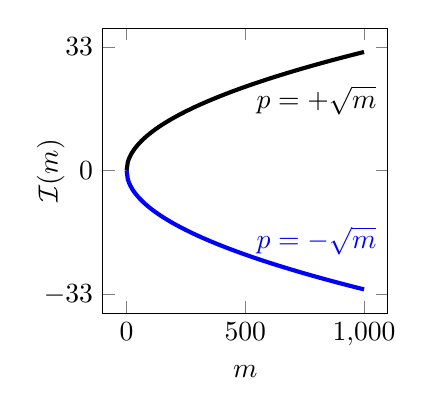
\begin{tikzpicture}
\begin{axis}
[scatter/classes={ a={mark=o,draw=blue}}, xlabel=$m$, ylabel=$\mathcal{I}(m)$,
y label style={at={(axis description cs:-0.1,0.5)},anchor=south},
  height=5.2cm,
  width=5.2cm,
  ytick={-33,0,33}]
\addplot[samples=200, line width=1.5pt, domain = 0:1000, color=black] plot(\x,{sqrt(\x)}) node[pos=0.8,inner sep=7pt, below] {$ p=+\sqrt{m} $};
\addplot[samples=200, line width=1.5pt, domain = 0:1000, color=blue] plot(\x,{-sqrt(\x)}) node[pos=0.8,inner sep=7pt, above] {$ p=-\sqrt{m} $};
\end{axis}
	%\draw[->] (-3,0)--(3,0) node[right]{$y$};
	%\draw[->] (0,-2)--(0,4) node[left]{$x$};
	%\draw[smooth, line width=1.5pt, domain = 0:3, color=blue] plot(\x,{sqrt(\x)}) node[right] {$ x=\sqrt{(x)} $};
	%\draw[smooth, line width=1.5pt, domain = 0:3, color=red] plot(\x,{-sqrt(\x)}) node[right] {$ y=-\sqrt{x} $};
\end{tikzpicture}
}
	%\caption{Model problem with known analytical solution.}
	%\label{fig:real_graphics}
\end{figure}
\end{frame}


\begin{frame}{Loss function: Data misfit}
%\vspace{-0.6 cm}
Definitions:
%\vspace{-0.2 cm}
\begin{flalign}
\hspace{3cm}
\notag
	& \mathcal{I} \;\;\:\: := \text{Inverse operator (Measurements $-->$ Earth properties)}  & \\
\notag
	& \mathcal{I}_{\phi^\ast} \: := \text{Neural Network approx. of }\mathcal{I} & 
\notag
\end{flalign}

Data misfit loss function:
\begin{flalign}
\hspace{3cm}
\notag
	 & \mathcal{I}_{\phi^\ast} \: := \arg \min_{\phi \in \Phi} \sum_i \|\mathcal{I}_{\phi}(\mathbf{m}_i)-\mathbf{p}_i\| & \\
	 \qquad
\notag
\end{flalign}
\end{frame}


\begin{frame}{Loss function: Data misfit}
\begin{figure}[!h]
\centering
	\subcaptionbox{$\left\Vert \cdot \right\Vert_{1}$-norm \label{fig:loss1_norm2}}{%
	\begin{tikzpicture}
\begin{axis}
[scatter/classes={ a={mark=o,draw=red}}, xlabel=$m$, ylabel=${\cal I}_{\theta^\ast}(m)$,
%y label style={at={(axis description cs:0.2,0.5)},anchor=south},
  legend pos=north west,
  legend style={draw=none,nodes={scale=0.5, transform shape}},
  height=5.2cm,
  width=5.2cm,
  ytick={-33,0,33}]
\addplot[scatter,only marks,%
    scatter src=explicit symbolic, color=red, mark=o]%
table[x,y] {Diapos/DL_For_Inv/Figures/Sqrt/DATA_FILES//DATA//Loss_1/Data_loss1_norm1} node[pos=.1,inner sep=7pt, above] { {\color{red} Predicted}};
%  \addlegendentry{Trained NN}
\addplot[solid,samples=200, line width=1.5pt, domain = 0:1100, color=black] plot(\x,{sqrt(\x)}) node[pos=0.7,inner sep=5pt, below] { {\color{black} Real}}; 
%  \addlegendentry{Ground Truth}
\addplot[solid,samples=200, line width=1.5pt, domain = 0:1100, color=black] plot(\x,{-sqrt(\x)});
\end{axis}
%\node at (1.65,4.2) {$L_1$ Norm};
\end{tikzpicture}



  
  
  
  
  
  
%\begin{tikzpicture}
%\begin{axis}
%[scatter/classes={ a={mark=o,draw=red}}, xlabel=$y$, ylabel=$\mathcal{I}_{h}(y)$,
%y label style={at={(axis description cs:0.2,0.5)},anchor=south},
%  height=5.8cm,
%  width=5.8cm,]
%\addplot[scatter,only marks,%
%    scatter src=explicit symbolic, color=red, mark=o]%
%table[x,y] {DATA_FILES//DATA//Loss_1//Data_loss1_norm1};
%\addplot[smooth, line width=1.5pt, domain = 0:1000, color=blue] plot(\x,{sqrt(\x)}); \label{legend:l1}
%\addplot[smooth, line width=1.5pt, domain = 0:1000, color=blue] plot(\x,{-sqrt(\x)});
%\end{axis}
%\end{tikzpicture}
}
	\hspace{0.3cm}
	\subcaptionbox{$\left\Vert \cdot \right\Vert_{2}$-norm \label{fig:loss1_norm1}}{%
	\begin{tikzpicture}
\begin{axis}
[scatter/classes={ a={mark=o,draw=red}}, xlabel=$m$,
   ylabel near ticks, ylabel=${\cal I}_{\theta^\ast}(m)$,
  % y label style={at={(axis description cs:-0.08,0.5)},anchor=south},
     legend pos=north west,
  legend style={draw=none,nodes={scale=0.5, transform shape}},
  height=5.2cm,
  width=5.2cm,
  ytick={-33,0,33}]
\addplot[scatter,only marks,%
    scatter src=explicit symbolic, color=red, mark=o]%
table[x,y] {Diapos/DL_For_Inv/Figures/Sqrt/DATA_FILES//DATA//Loss_1//Data_loss1_norm2} node[pos=.1,inner sep=7pt, above] { {\color{red} Predicted}};
%  \addlegendentry{Trained NN}
\addplot[solid,samples=200, line width=1.5pt, domain = 0:1100, color=black] plot(\x,{sqrt(\x)}) node[pos=0.7,inner sep=5pt, below] { {\color{black} Real}}; 
 % \addlegendentry{Ground Truth}
\addplot[smooth,samples=200, line width=1.5pt, domain = 0:1100, color=black] plot(\x,{-sqrt(\x)});
\end{axis}
%\node at (1.65,4.2) {$L_2$ Norm};
\end{tikzpicture}
}
	%\caption{Analytical solution vs DNN predicted solution evaluated over the test dataset using the loss function based on the data misfit.}
	%\label{fig:loss1}
\end{figure}
\end{frame}


\begin{frame}[t]{$|| \cdot ||_2$-norm}
\visible<1-4>{For every sample of the form $(m_i,p_i)=(m_i, \sqrt{m_i})$, there exists another one $(m_i, -\sqrt{m_i})$.}
\vspace{0.3cm}

\visible<2-4>{Then, for a specific sample $m$, the solution that minimizes the loss must satisfy
\begin{equation}
(\mathcal{I}_{{\cal R},\theta}(m) - \sqrt{m})^2 + (\mathcal{I}_{{\cal R},\theta}(m) - (-\sqrt{m}))^2.
\label{eq:norm2_proof_2}
\end{equation}}

\visible<3-4>{Taking the derivative of Eq. (\ref{eq:norm2_proof_2}) with respect to $\mathcal{I}_{{\cal R},\theta}(m)$ and equaling it to zero, we obtain
\begin{equation}
4\cdot\mathcal{I}_{{\cal R},\theta}(m)= 0.
\label{eq:loss1_norm2_derived}
\end{equation}}

\visible<4-4>{Thus, for any sample $m_i$, the function is minimized when the approximated value is $\mathcal{I}_{{\cal R},\theta}(m_i)=0$.}
\end{frame}


\begin{frame}{Loss function: Desired}
%\vspace{-0.6 cm}

Definitions:
%\vspace{-0.2 cm}
\begin{flalign}
\hspace{3cm}
\notag
	& \mathcal{F} \;\;\: := \text{Forward operator (Earth properties $-->$ Measurements)}  & \\
\notag
	& \mathcal{I} \;\;\:\: := \text{Inverse problem (Measurements $-->$ Earth properties)}  & \\
\notag
	& \mathcal{I}_{\phi^\ast} \: := \text{Neural Network approx. of }\mathcal{I} & 
\notag
\end{flalign}

Desired loss function:
\begin{flalign}
\hspace{3cm}
\notag
	 & \mathcal{I}_{\phi^\ast} \: := \arg \min_{\phi \in \Phi} \sum_i \|(\mathcal{F} \circ \mathcal{I}_{\phi})(\mathbf{m}_i)-\mathbf{m}_i \| & \\
	 \qquad
\notag
\end{flalign}

\visible<2>{\centerline{\textcolor{red}{Evaluating $\mathcal{F}$  is expensive}}}
\end{frame}


\begin{frame}{Loss function: Encoder-Decoder}
%\vspace{-0.6 cm}

Definitions:
%\vspace{-0.2 cm}
\begin{flalign}
\hspace{3cm}
\notag
	& \mathcal{F} \;\;\: := \text{Forward operator (Earth properties $-->$ Measurements)}  & \\
\notag
	& \mathcal{I} \;\;\:\: := \text{Inverse operator (Measurements $-->$ Earth properties)}  & \\
\notag
	& \mathcal{F}_{\theta^\ast}:= \text{Neural Network approx. of }\mathcal{F} & \\
	& \mathcal{I}_{\phi^\ast} \: := \text{Neural Network approx. of }\mathcal{I} & 
\notag
\end{flalign}

Encoder-Decoder loss function:
\begin{flalign}
\hspace{3cm}
\notag
	 \{ \mathcal{I}_{\phi^\ast},\mathcal{F}_{\theta^\ast} \}:= & \arg \min_{\shortstack{$\scriptstyle \theta \in \Theta$ \\ $\scriptstyle \phi \in \Phi$}}  \sum_i ( \|(\mathcal{F}_{\theta} \circ \mathcal{I}_{\phi})(\mathbf{m}_i)-\mathbf{m}_i \|  + \|{\cal F}_{\theta}(\mathbf{p}_i)-\mathbf{m}_i \| )& \\
%	 & + \|{\cal F}_{\theta}(\mathbf{z}_i)-\mathbf{m}_i \| ) &
\notag
\end{flalign}
\end{frame}


\begin{frame}{Loss function: Encoder-Decoder}
\begin{figure}[!h]
\centering
	\subcaptionbox{$\left\Vert \cdot \right\Vert_{1}$-norm \label{fig:loss1_norm2}}{%
	\begin{tikzpicture}
\begin{axis}
[scatter/classes={ a={mark=o,draw=red}}, xlabel=$m$, ylabel=$ {\cal I}_{\theta^\ast}(m) $,
%y label style={at={(axis description cs:0.2,0.5)},anchor=south},
  legend pos=north west,
  legend style={draw=none,nodes={scale=0.5, transform shape}},
  height=5.2cm,
  width=5.2cm,
  ytick={-33,0,33}]
\addplot[scatter,only marks,%
    scatter src=explicit symbolic, color=red, mark=o]%
table[x,y] {Diapos/DL_For_Inv/Figures/Sqrt/DATA_FILES//DATA//Loss_4//Norm_1//Data_INV_loss4_norm1} node[pos=.1,inner sep=12pt, above] { {\color{red} Predicted}};
 % \addlegendentry{Trained NN}
\addplot[solid,samples=200, line width=1.5pt, domain = 0:1100, color=black] plot(\x,{sqrt(\x)}) node[pos=0.7,inner sep=5pt, below] { {\color{black} Real}}; 
 % \addlegendentry{Ground Truth}
\addplot[solid,samples=200, line width=1.5pt, domain = 0:1100, color=black] plot(\x,{-sqrt(\x)});
\end{axis}
%\node at (1.65,4.2) {$L_1$ Norm};
\end{tikzpicture}
}
	\hspace{0.3cm}
	\subcaptionbox{$\left\Vert \cdot \right\Vert_{2}$-norm \label{fig:loss1_norm1}}{%
	\begin{tikzpicture}
\begin{axis}
[scatter/classes={ a={mark=o,draw=red}}, xlabel=$m$, ylabel=$ {\cal I}_{\theta^\ast}(m) $,
%y label style={at={(axis description cs:0.2,0.5)},anchor=south},
  legend pos=north west,
  legend style={draw=none,nodes={scale=0.5, transform shape}},
  height=5.2cm,
  width=5.2cm,
  ytick={-33,0,33}]
\addplot[scatter,only marks,%
    scatter src=explicit symbolic, color=red, mark=o]%
table[x,y] {Diapos/DL_For_Inv/Figures/Sqrt/DATA_FILES//DATA//Loss_4//Norm_2//Data_INV_loss4_norm2} node[pos=.1,inner sep=12pt, below] { {\color{red} Predicted}};
%  \addlegendentry{Trained NN}
\addplot[solid,samples=200, line width=1.5pt, domain = 0:1100, color=black] plot(\x,{sqrt(\x)}); 
%  \addlegendentry{Ground Truth}
\addplot[solid,samples=200, line width=1.5pt, domain = 0:1100, color=black] plot(\x,{-sqrt(\x)}) node[pos=0.7,inner sep=5pt, above] { {\color{black} Real}};
\end{axis}
%\node at (1.65,4.2) {$L_2$ Norm};
\end{tikzpicture}
}
	%\caption{Analytical solution vs DNN predicted solution evaluated over the test dataset using the loss function based on the data misfit.}
	%\label{fig:loss1}
\end{figure}
\end{frame}


\begin{frame}{Loss function: Two-Step}
%\vspace{-0.6 cm}
Definitions:
%\vspace{-0.2 cm}
\begin{flalign}
\hspace{3cm}
\notag
	& \mathcal{F} \;\;\: := \text{Forward operator (Earth properties $-->$ Measurements)}  & \\
\notag
	& \mathcal{I} \;\;\:\: := \text{Inverse operator (Measurements $-->$ Earth properties)}  & \\
\notag
	& \mathcal{F}_{\theta^\ast}:= \text{Neural Network approx. of }\mathcal{F} & \\
	& \mathcal{I}_{\phi^\ast} \: := \text{Neural Network approx. of }\mathcal{I} & 
\notag
\end{flalign}

Two-step loss function:
\begin{flalign}
\hspace{3cm}
\notag
	& \mathcal{F}_{\theta^\ast}:= \arg \min_{\theta \in \Theta}  \sum_i \|{\cal F}_{\theta}(\mathbf{p}_i)-\mathbf{m}_i \| & \\
	 & \mathcal{I}_{\phi^\ast} \: := \arg \min_{\phi \in \Phi} \sum_i \|(\mathcal{F}_{\theta^\ast} \circ \mathcal{I}_{\phi})(\mathbf{m}_i)-\mathbf{m}_i \| &
\notag
\end{flalign}
\end{frame}


\begin{frame}{Loss function: Two-Step}
\begin{figure}[!h]
\centering
	\subcaptionbox{$\left\Vert \cdot \right\Vert_{1}$-norm \label{fig:loss1_norm2}}{%
	\begin{tikzpicture}
\begin{axis}
[scatter/classes={ a={mark=o,draw=red}}, xlabel=$m$, ylabel=$ {\cal I}_{\theta^\ast}(m) $,
%y label style={at={(axis description cs:0.2,0.5)},anchor=south},
  legend pos=north west,
  legend style={draw=none,nodes={scale=0.5, transform shape}},
  height=5.2cm,
  width=5.2cm,
  ytick={-33,0,33}]
\addplot[scatter,only marks,%
    scatter src=explicit symbolic, color=red, mark=o]%
table[x,y] {Diapos/DL_For_Inv/Figures/Sqrt/DATA_FILES//DATA//Loss_5//Norm_1//Data_INV_loss5_norm1} node[pos=.1,inner sep=12pt, below] { {\color{red} Predicted}};
%  \addlegendentry{Trained NN}
\addplot[solid,samples=200, line width=1.5pt, domain = 0:1100, color=black] plot(\x,{sqrt(\x)}); 
%  \addlegendentry{Ground Truth}
\addplot[solid,samples=200, line width=1.5pt, domain = 0:1100, color=black] plot(\x,{-sqrt(\x)}) node[pos=0.7,inner sep=5pt, above] { {\color{black} Real}};
\end{axis}
%\node at (1.65,4.2) {$L_1$ Norm};
\end{tikzpicture}
}
	\hspace{0.3cm}
	\subcaptionbox{$\left\Vert \cdot \right\Vert_{2}$-norm \label{fig:loss1_norm1}}{%
	\begin{tikzpicture}
\begin{axis}
[scatter/classes={ a={mark=o,draw=red}}, xlabel=$m$, ylabel=$ {\cal I}_{\theta^\ast}(m) $,
%y label style={at={(axis description cs:0.2,0.5)},anchor=south},
  legend pos=north west,
  legend style={draw=none,nodes={scale=0.5, transform shape}},
  height=5.2cm,
  width=5.2cm,
  ytick={-33,0,33}]
\addplot[scatter,only marks,%
    scatter src=explicit symbolic, color=red, mark=o]%
table[x,y] {Diapos/DL_For_Inv/Figures/Sqrt/DATA_FILES//DATA//Loss_5//Norm_2//Data_INV_loss5_norm2} node[pos=.1,inner sep=12pt, below] { {\color{red} Predicted}};
%  \addlegendentry{Trained NN}
\addplot[solid,samples=200, line width=1.5pt, domain = 0:1100, color=black] plot(\x,{sqrt(\x)}); 
%  \addlegendentry{Ground Truth}
\addplot[solid,samples=200, line width=1.5pt, domain = 0:1100, color=black] plot(\x,{-sqrt(\x)}) node[pos=0.7,inner sep=5pt, above] { {\color{black} Real}};
\end{axis}
%\node at (1.65,4.2) {$L_2$ Norm};
\end{tikzpicture}
}
	%\caption{Analytical solution vs DNN predicted solution evaluated over the test dataset using the loss function based on the data misfit.}
	%\label{fig:loss1}
\end{figure}
\end{frame}



%%%%%%%%%
{
\usebackgroundtemplate{\tikz\node[opacity=0.1,inner sep=0] {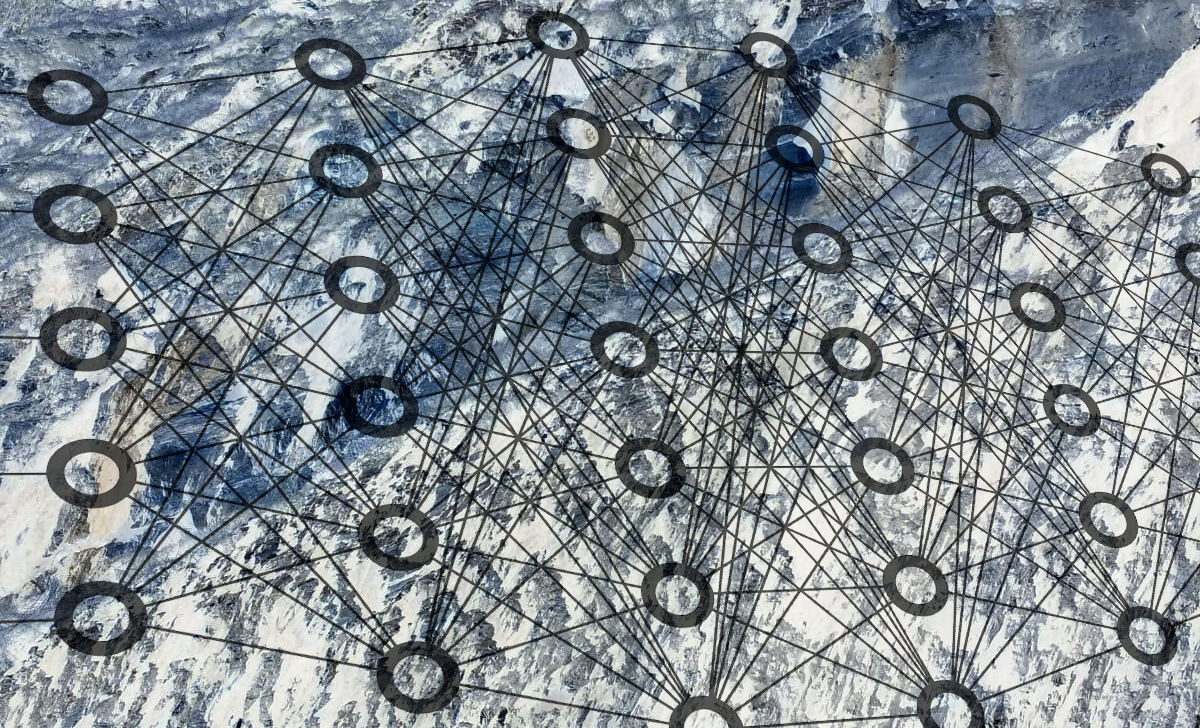
\includegraphics[height=\paperheight,width=\paperwidth]{frames/auxiliar/title_img/prueba.png}};}

\begin{frame}[plain]
\begin{variableblock}{}{bg=myblue,fg=white}{bg=green,fg=red}
\begin{center}
\textbf{Geophysics Synthetic Example}
\end{center}
\end{variableblock}
\end{frame}
}
%%%%%%%%%%%%%%%%%%%%%%%%%%%%%%%%%%%%%%%%%%%%%%%%%%%%%%%%%%%%%%%%%%%
%\def\layersep{1.5cm}

\def\checkmark{\tikz\fill[scale=0.8, color=green_jon](0,.35) -- (.25,0) -- (1,.7) -- (.25,.15) -- cycle;} 
\definecolor{green_jon}{rgb}{0.0, 0.5, 0.0}

\begin{frame}{Geophysics Synthetic Example: Input Measurements}
\vspace{-0.35 cm}
\begin{figure}[H]
	\centering
	\begin{tikzpicture}[scale=1.0]
	\node (layers) at (0.0,0.0)[scale=0.7]{
		\begin{tikzpicture}

%% Tool
\fill[gray!80!white] (-1.5*3,0) -- (1.5*3,0.) --  node[right] {\small \bf \textcolor{black}{500 kHz}}  (1.5*3, 0.15*3) -- (-1.5*3,0.15*3) -- cycle;

%% Transmitters
\fill[black!80!white] (-0.6096*5-0.02*3,0) -- (-0.6096*5+0.02*3,0.) -- (-0.6096*5+0.02*3, 0.15*3) node[above] {\footnotesize \bf \textcolor{black}{Tx$_1$}}  -- (-0.6096*5-0.02*3,0.15*3) -- cycle;
%
\fill[black!80!white] (0.6096*5-0.02*3,0) -- (0.6096*5+0.02*3,0.)  -- (0.6096*5+0.02*3, 0.15*3) node[above] {\footnotesize \bf \textcolor{black}{Tx$_2$}} -- (0.6096*5-0.02*3,0.15*3) -- cycle;

%% Receivers
\fill[red!80!white] (-0.1016*5-0.02*3,0) -- (-0.1016*5+0.02*3,0.)  -- (-0.1016*5+0.02*3, 0.15*3) node[above] {\footnotesize \bf \textcolor{black}{Rx$_1$}} -- (-0.1016*5-0.02*3,0.15*3) -- cycle;
\fill[red!80!white] ( 0.1016*5-0.02*3,0) -- ( 0.1016*5+0.02*3,0.) -- ( 0.1016*5+0.02*3, 0.15*3)  node[above] {\footnotesize \bf \textcolor{black}{Rx$_2$}} -- ( 0.1016*5-0.02*3,0.15*3) -- cycle;

%% distances
\draw[black, line width=1pt,<->] (-0.1016*5, -0.6)      -- (0.1016*5, -0.6) node[pos=0.5, below] {\footnotesize \bf \textcolor{black}{0.40 m}}  ;
\draw[gray, dashed] (-0.1016*5, -0.6)      -- (-0.1016*5, 0)  ;
\draw[gray, dashed] ( 0.1016*5, -0.6)      -- ( 0.1016*5, 0)  ;

\draw[black, line width=1pt,<->] (-0.6096*5, -1.2)      -- (0.6096*5, -1.2) node[pos=0.5, below] {\footnotesize \bf \textcolor{black}{1.8 m}}  ;
\draw[gray, dashed] (-0.6096*5,-1.2)      -- (-0.6096*5, 0)  ;
\draw[gray, dashed] ( 0.6096*5,-1.2)      -- ( 0.6096*5, 0)  ;


\end{tikzpicture}
	};       
	\end{tikzpicture}
\end{figure}
\vspace{-0.7 cm}

	\begin{itemize}
		\item Co-axial attenuation and phase difference
	\end{itemize}
	
	\vspace{0.4 cm}

\begin{figure}[H]
	\centering
	\begin{tikzpicture}[scale=1.0]
	\node (layers) at (0.0,0.0)[scale=0.7]{
		\begin{tikzpicture}

%% Tool
\fill[gray!80!white] (-1.7*3,0) -- (1.7*3,0.) --  node[right] {\small \bf \textcolor{black}{10 kHz}}  (1.7*3, 0.15*3) -- (-1.7*3,0.15*3) -- cycle;

%% Transmitters
\fill[black!80!white] (-0.6096*5-0.02*3,0) -- (-0.6096*5+0.02*3,0.) -- (-0.6096*5+0.02*3, 0.15*3) node[above] {\footnotesize \bf \textcolor{black}{Tx}}  -- (-0.6096*5-0.02*3,0.15*3) -- cycle;
%
\fill[red!80!white] (0.6096*5-0.02*3,0) -- (0.6096*5+0.02*3,0.)  -- (0.6096*5+0.02*3, 0.15*3) node[above] {\footnotesize \bf \textcolor{black}{Rx}} -- (0.6096*5-0.02*3,0.15*3) -- cycle;

%% Receivers
%\fill[red!80!white] (-0.1016*5-0.02*3,0) -- (-0.1016*5+0.02*3,0.)  -- (-0.1016*5+0.02*3, 0.15*3) node[above] {\footnotesize \bf \textcolor{black}{Rx$_1$}} -- (-0.1016*5-0.02*3,0.15*3) -- cycle;
%\fill[red!80!white] ( 0.1016*5-0.02*3,0) -- ( 0.1016*5+0.02*3,0.) -- ( 0.1016*5+0.02*3, 0.15*3)  node[above] {\footnotesize \bf \textcolor{black}{Rx$_2$}} -- ( 0.1016*5-0.02*3,0.15*3) -- cycle;

%% distances
%\draw[black, line width=1pt,<->] (-0.1016*5, -0.6)      -- (0.1016*5, -0.6) node[pos=0.5, below] {\footnotesize \bf \textcolor{black}{0.40 m}}  ;
%\draw[gray, dashed] (-0.1016*5, -0.6)      -- (-0.1016*5, 0)  ;
%\draw[gray, dashed] ( 0.1016*5, -0.6)      -- ( 0.1016*5, 0)  ;

\draw[black, line width=1pt,<->] (-0.6096*5, -0.7)      -- (0.6096*5, -0.7) node[pos=0.5, below] {\footnotesize \bf \textcolor{black}{12 m}}  ;
\draw[gray, dashed] (-0.6096*5,-0.7)      -- (-0.6096*5, 0)  ;
\draw[gray, dashed] ( 0.6096*5,-0.7)      -- ( 0.6096*5, 0)  ;


\end{tikzpicture}
	};       
	\end{tikzpicture}
\end{figure}
\vspace{-0.7 cm}
	\begin{itemize}
		\item Co-axial attenuation and phase difference
		\item Geosignal
	\end{itemize}
\end{frame}


\begin{frame}{Geophysics Synthetic Example: Output Earth Parametrization}
\begin{columns}
    \begin{column}{0.35\textwidth}
    \begin{figure}[!h]
	\centering
	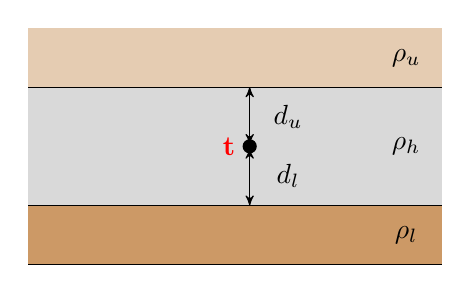
\begin{tikzpicture}[scale=1.5]
\draw (0,0) rectangle (3.5,2);

\fill[white!20!brown] (0,0) rectangle (3.5,0.5);
\fill[white!70!gray] (0,0.5) rectangle (3.5,1.5);
\fill[white!60!brown] (0,1.5) rectangle (3.5,2);


%\draw[red, line width=0.5 mm] (0.75,1.5) .. controls (1.15,1.1) .. (1.85,1) node (n1) at (0.85,1.6) {$\mathbf{t}$};
\draw[black, line width=0.1 mm] (0,0.5) -- (3.5,0.5);
\draw[black, line width=0.1 mm] (0,1.5) -- (3.5,1.5);

\fill[black] (1.875,1) circle (0.06cm);
\node (d_u) at (1.7,1) {\textcolor{red}{$\textbf{t}$}};
\draw[<->] (1.875,1.02) -- (1.875,1.5);
\node (d_u) at (2.2,1.25) {$d_u$}; 
\draw[<->] (1.875,0.98) -- (1.875,.5);
\node (d_u) at (2.2,0.75) {$d_l$};
\node (rho) at (3.2,1.75) {$\rho_u$};
\node (rho) at (3.2,0.25) {$\rho_l$};
\node (rho) at (3.2,1) {$\rho_h$};
\end{tikzpicture}

	\label{fig:param}
	\end{figure}
    \end{column}
    \begin{column}{0.5\textwidth}
        {\footnotesize $\rho_u \in [1,10^2] \Omega \cdot m$: Upper layer resistivity}\\
        \vspace{0.3cm}
        {\footnotesize $\rho_h \in [1,10^2] \Omega \cdot m$: Central layer resistivity}\\
        \vspace{0.3cm}
        {\footnotesize $\rho_l \in [1,10^2] \Omega \cdot m$: Lower layer resistivity}\\
        \vspace{0.3cm}
        {\footnotesize $d_u \in [10^{-2},10] m$: Vertical distance to upper layer}\\
        \vspace{0.3cm}
        {\footnotesize $d_l \in [10^{-2},10] m$: Vertical distance to lower layer}
    \end{column}
\end{columns}
\end{frame}



\begin{frame}{Synthetic Example}
\begin{center}
{\large Formation of model problem}
\end{center}
\begin{figure}
		\centering
		\pgfplotsset{every axis legend/.append style={
		at={(0.5,1.03)},
		anchor=south},
	every axis plot/.append style={line width=1.8pt},
}
\begin{tikzpicture}
\begin{axis}[
%  ymode=log,
%  xmode=log,
%  grid=both,
%xmin=0,
%xmax=540,
legend columns=2,
%  ymin=-20.0,
%  ymax=-11,
height=0.3*\textwidth,
width=0.85*\textwidth,
% 
y dir=reverse,
xlabel={HD ($m$)},
ylabel near ticks,
ylabel={TVD ($m$)},
%axis equal image,
enlargelimits=false,
]

%[enlargelimits=false, axis on top, axis equal image, width=6cm]

%\node[] at (rel axis cs:0,0) {\includegraphics{Syn_1/Predicted.png}};

\addplot graphics[xmin=0,xmax=540,ymin=45,ymax=60] {Diapos/DL_For_Inv/Figures/Syn_example/Numerical_results/Real.png};

\end{axis}	
\end{tikzpicture}

	%\caption{Formation of model problem}
	\label{fig:formation_model_1_original}
\end{figure}
\end{frame}


\begin{frame}{Encoder-Decoder Loss}
\begin{center}
Predicted formation
\end{center}
\begin{figure}
		\centering
		\pgfplotsset{every axis legend/.append style={
		at={(0.5,1.03)},
		anchor=south},
	every axis plot/.append style={line width=1.8pt},
}
\begin{tikzpicture}
\begin{axis}[
%  ymode=log,
%  xmode=log,
%  grid=both,
%xmin=0,
%xmax=540,
legend columns=2,
%  ymin=-20.0,
%  ymax=-11,
height=0.23*\textwidth,
width=0.75*\textwidth,
% 
 y dir=reverse,
xlabel={HD ($m$)},
ylabel near ticks,
ylabel={TVD ($m$)},
%axis equal image,
enlargelimits=false,
]

%[enlargelimits=false, axis on top, axis equal image, width=6cm]

%\node[] at (rel axis cs:0,0) {\includegraphics{Syn_1/Predicted.png}};

\addplot graphics[xmin=0,xmax=540,ymin=45,ymax=60] {Diapos/DL_For_Inv/Figures/Syn_example/Numerical_results/Enco-Deco/Predicted_F_FI.png};

\end{axis}	
\end{tikzpicture}

	%\caption{Formation of model problem}
	\label{fig:formation_model_1_original}
\end{figure}
\begin{center}
Geosignal measurement
\end{center}
\begin{figure}
		\centering
		\pgfplotsset{every axis legend/.append style={
		at={(0.5,1.03)},
		anchor=south},
	every axis plot/.append style={line width=1.8pt},
}
\begin{tikzpicture}
\begin{axis}[
%  ymode=log,
%  xmode=log,
%  grid=both,
xmin=0,
xmax=540,
legend columns=2,
%  ymin=-20.0,
%  ymax=-11,
height=0.23*\textwidth,
width=0.75*\textwidth,
%  y dir=reverse,
xlabel={HD ($m$)},
ylabel near ticks,
ylabel={Att. ($dB$)},
]
\addplot[blue,line width=1] table [x=X, y expr=(\thisrow{Atten_Geosignal} + 1.84)*8.68 ]{Diapos/DL_For_Inv/Figures/Syn_example/Numerical_results/Enco-Deco/F_aI_b.dat}
node[pos=0.8,inner sep=12pt, above,align=center,font=\linespread{1.0}\selectfont] { {\color{blue} ${\cal F} \circ {\cal I}$}
	{\color{black} vs} {\color{red} ${\cal F} \circ {\cal I}_{\theta^\ast}$}};

\addplot[red,dashed,line width=1] table [x=X, y expr=(\thisrow{Atten_Geosignal} + 1.84)*8.68 ]{Diapos/DL_For_Inv/Figures/Syn_example/Numerical_results/Enco-Deco/FI_b_without_regularization.dat};

\end{axis}	
\end{tikzpicture}

	%\caption{Formation of model problem}
	\label{fig:formation_model_1_original}
\end{figure}
\end{frame}


\begin{frame}{Encoder-Decoder Loss}
%\vspace{-0.5cm}
\begin{equation}
\begin{aligned}
	(\mathcal{F}_{\theta^\ast}, \mathcal{I}_{\phi^\ast}):=\arg \min_{\phi \in \Phi, \theta \in \Theta} \{ & \|(\mathcal{F}_{\theta} \circ \textcolor{blue}{\mathcal{I}_{\phi}})(\mathbf{M})-\mathbf{M}\| + \textcolor{green_jon}{\|{\cal F}_{\theta}({\bf P})-{\bf M}\|} \}
\end{aligned}
\notag
\end{equation}

\begin{figure}[!h]
	\centering
	\begin{tikzpicture}[scale=0.7]
\tikzset{cross/.style={cross out, draw=green_jon, minimum size=0.2cm, inner sep=0pt, outer sep=0pt},
%default radius will be 1pt. 
cross/.default={1pt}}

\draw (0,0) rectangle (8,4);
\node[left] at (0,4) {$\rho_l$};
\node[below] at (8,0) {$\rho_u$};

\draw (1,1) node[cross] {};
\draw (1,2) node[cross] {};
\draw (1,3) node[cross] {};

\draw (3,1) node[cross] {};
\draw (3,2) node[cross] {};
\draw (3,3) node[cross] {};

\draw (5,1) node[cross] {};
\draw (5,2) node[cross] {};
\draw (5,3) node[cross] {};

\draw (7,1) node[cross] {};
\draw (7,2) node[cross] {};
\draw (7,3) node[cross] {};

\draw (4,2) node[circle,draw=blue,minimum size=0.1cm] {};

\end{tikzpicture}



	\label{fig:regu}
\end{figure}

\center
\textcolor{green_jon}{x}=training samples

${\cal F}_\theta(\textcolor{green_jon}{x}) \approx {\cal F}(\textcolor{green_jon}{x})$

${\cal F}_\theta(\textcolor{blue}{O}) \neq {\cal F}(\textcolor{blue}{O})$
%\vspace{0.5cm}
\end{frame}


\begin{frame}{Two-Step Loss}
\begin{center}
Predicted formation
\end{center}
\begin{figure}[!h]
				\centering
	\pgfplotsset{every axis legend/.append style={
		at={(0.5,1.03)},
		anchor=south},
	every axis plot/.append style={line width=1.8pt},
}
\begin{tikzpicture}
\begin{axis}[
%  ymode=log,
%  xmode=log,
%  grid=both,
%xmin=0,
%xmax=540,
legend columns=2,
%  ymin=-20.0,
%  ymax=-11,
height=0.23*\textwidth,
width=0.75*\textwidth,
% 
 y dir=reverse,
xlabel={HD ($m$)},
ylabel near ticks,
ylabel={TVD ($m$)},
%axis equal image,
enlargelimits=false,
]

%[enlargelimits=false, axis on top, axis equal image, width=6cm]

%\node[] at (rel axis cs:0,0) {\includegraphics{Syn_1/Predicted.png}};

\addplot graphics[xmin=0,xmax=540,ymin=45,ymax=60] {Diapos/DL_For_Inv/Figures/Syn_example/Numerical_results/Two_Step/Predicted_F_FI_two_step.png};

\end{axis}	
\end{tikzpicture}
%
	%\caption{Predicted formation using the Encoder-Decoder loss function with regularization}
\end{figure}
\begin{center}
Geosignal measurement
\end{center}
\begin{figure}[!h]
	\centering
	\pgfplotsset{every axis legend/.append style={
		at={(0.5,1.03)},
		anchor=south},
	every axis plot/.append style={line width=1.8pt},
}
\begin{tikzpicture}
\begin{axis}[
%  ymode=log,
%  xmode=log,
%  grid=both,
xmin=0,
xmax=540,
legend columns=2,
%  ymin=-20.0,
%  ymax=-11,
height=0.23*\textwidth,
width=0.75*\textwidth,
%  y dir=reverse,
xlabel={HD ($m$)},
ylabel near ticks,
ylabel={Att. ($dB$)},
]
\addplot[blue,line width=1] table [x=X, y expr=(\thisrow{Atten_Geosignal} + 1.84)*8.68 ]{Diapos/DL_For_Inv/Figures/Syn_example/Numerical_results/Two_Step/F_aI_b.dat}
node[pos=0.8,inner sep=12pt, above,align=center,font=\linespread{1.0}\selectfont] { {\color{blue} ${\cal F} \circ {\cal I}$}
	{\color{black} vs} {\color{red} ${\cal F} \circ {\cal I}_{\theta^\ast}$}};

\addplot[red,dashed,line width=1] table [x=X, y expr=(\thisrow{Atten_Geosignal} + 1.84)*8.68 ]{Diapos/DL_For_Inv/Figures/Syn_example/Numerical_results/Two_Step/FI_b_two_step.dat};

\end{axis}	
\end{tikzpicture}
%
	%\caption{Deep coaxial measurement}
\end{figure}
\end{frame}


%==========================================================
\begin{frame}{Cross-plot}
\centering
\setlength{\fboxrule}{0.5mm}
\setlength{\fboxsep}{1mm}
\color{red}
\fbox{\parbox{3cm}{{\begin{align}
\textcolor{black}
{\mathcal{I} \hspace{0.25cm} vs \hspace{0.25cm} \mathcal{I}_{\phi^\ast}}
\notag
\end{align}}}}
\color{black}

$\qquad$ \\
\hspace{0.5cm} $d_u$ $\qquad \qquad \qquad \qquad \qquad$ $\rho_h$ $\qquad \qquad \qquad \qquad \qquad$ $\rho_u$
\begin{figure}[!h]
\centering
	{%
		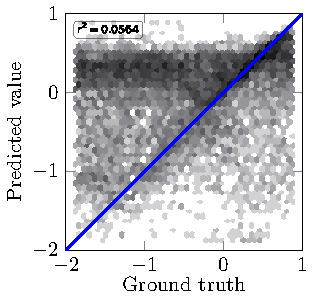
\includegraphics[scale=0.8]{Diapos/DL_For_Inv/Figures/Syn_example/Cross_plots/Two_Step_loss/C_P_4/d_u.pdf}
		\hspace{0.1cm}
		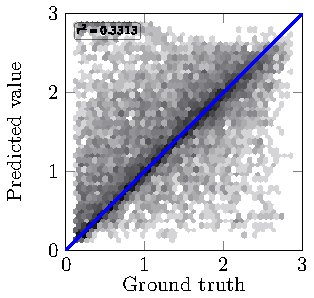
\includegraphics[scale=0.8]{Diapos/DL_For_Inv/Figures/Syn_example/Cross_plots/Two_Step_loss/C_P_4/rho_h.pdf}
		\hspace{0.1cm}
		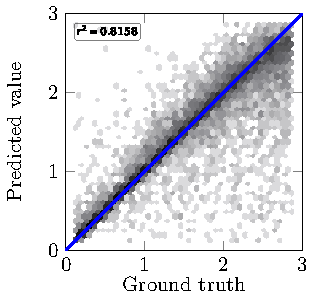
\includegraphics[scale=0.8]{Diapos/DL_For_Inv/Figures/Syn_example/Cross_plots/Two_Step_loss/C_P_4/rho_u.pdf}
		}	
\end{figure}	
\end{frame}


\begin{frame}{Encoder-Decoder Loss Regularization}
\begin{equation}
\begin{aligned}
	(\mathcal{F}_{\theta^\ast}, \mathcal{I}_{\phi^\ast}):=\arg \min_{\phi \in \Phi, \theta \in \Theta} \{ & \|(\mathcal{F}_{\theta} \circ \mathcal{I}_{\phi})(\mathbf{M})-\mathbf{M}\| +\|{\cal F}_{\theta}({\bf P})-{\bf M}\|\\
	&  + \textcolor{red}{\|{\cal I}_{\phi}({\bf M})-{\bf P}\| } \}
\end{aligned}
\notag
\end{equation} \\
\vspace{0.2cm}

\begin{figure}[!h]
				\centering
	\pgfplotsset{every axis legend/.append style={
		at={(0.5,1.03)},
		anchor=south},
	every axis plot/.append style={line width=1.8pt},
}
\begin{tikzpicture}
\begin{axis}[
%  ymode=log,
%  xmode=log,
%  grid=both,
%xmin=0,
%xmax=540,
legend columns=2,
%  ymin=-20.0,
%  ymax=-11,
height=0.23*\textwidth,
width=0.75*\textwidth,
% 
 y dir=reverse,
xlabel={HD ($m$)},
ylabel near ticks,
ylabel={TVD ($m$)},
%axis equal image,
enlargelimits=false,
]

%[enlargelimits=false, axis on top, axis equal image, width=6cm]

%\node[] at (rel axis cs:0,0) {\includegraphics{Syn_1/Predicted.png}};

\addplot graphics[xmin=0,xmax=540,ymin=45,ymax=60] {Diapos/DL_For_Inv/Figures/Syn_example/Numerical_results/Enco-Deco_REG/Predicted_F_FI_reg.png};

\end{axis}	
\end{tikzpicture}
%
	%\caption{Predicted formation using the Encoder-Decoder loss function with regularization}
\end{figure}

\begin{figure}[!h]
				\centering
	\pgfplotsset{every axis legend/.append style={
		at={(0.5,1.03)},
		anchor=south},
	every axis plot/.append style={line width=1.8pt},
}
\begin{tikzpicture}
\begin{axis}[
%  ymode=log,
%  xmode=log,
%  grid=both,
xmin=0,
xmax=540,
legend columns=2,
%  ymin=-20.0,
%  ymax=-11,
height=0.23*\textwidth,
width=0.75*\textwidth,
%  y dir=reverse,
xlabel={HD ($m$)},
ylabel near ticks,
ylabel={Att. ($dB$)},
]
\addplot[blue,line width=1] table [x=X, y expr=(\thisrow{Atten_Geosignal} + 1.84)*8.68 ]{Diapos/DL_For_Inv/Figures/Syn_example/Numerical_results/Enco-Deco_REG/F_aI_b.dat}
node[pos=0.8,inner sep=8pt, above,align=center,font=\linespread{1.0}\selectfont] { {\color{blue} ${\cal F} \circ {\cal I}$}
	{\color{black} vs} {\color{red} ${\cal F} \circ {\cal I}_{\theta^\ast}$}};

\addplot[red,dashed,line width=1] table [x=X, y expr=(\thisrow{Atten_Geosignal} + 1.84)*8.68 ]{Diapos/DL_For_Inv/Figures/Syn_example/Numerical_results/Enco-Deco_REG/FI_b.dat};

\end{axis}	
\end{tikzpicture}
%
	%\caption{Predicted formation using the Encoder-Decoder loss function with regularization}
\end{figure}
\end{frame}


\begin{frame}{Deep Learning for Inverse Borehole Problems}
\begin{itemize}
\item Deep Learning (DL) is an adequate option to invert borehole resistivity measurements in real time.
\vspace{0.5cm}
\item Traditional loss functions are not effective.
\vspace{0.5cm}
\item Both Encoder-Decoder and Two-Step are adequate alternatives.
\vspace{0.5cm}
\item Encoder-Decoder demands a regularization term.
\end{itemize}
\end{frame}
%\end{section}
%%%%%%%%%%%%%%%%%%%%%%%%%%%%%%%%%%
%%%%%%%%%%%%%%%%%%%%%%%%%%%%%%%%%%
%\begin{section}{Database Generation for Borehole Inversion Problems using rIGA}
%%%%%%%%%
{
\usebackgroundtemplate{\tikz\node[opacity=0.1,inner sep=0] {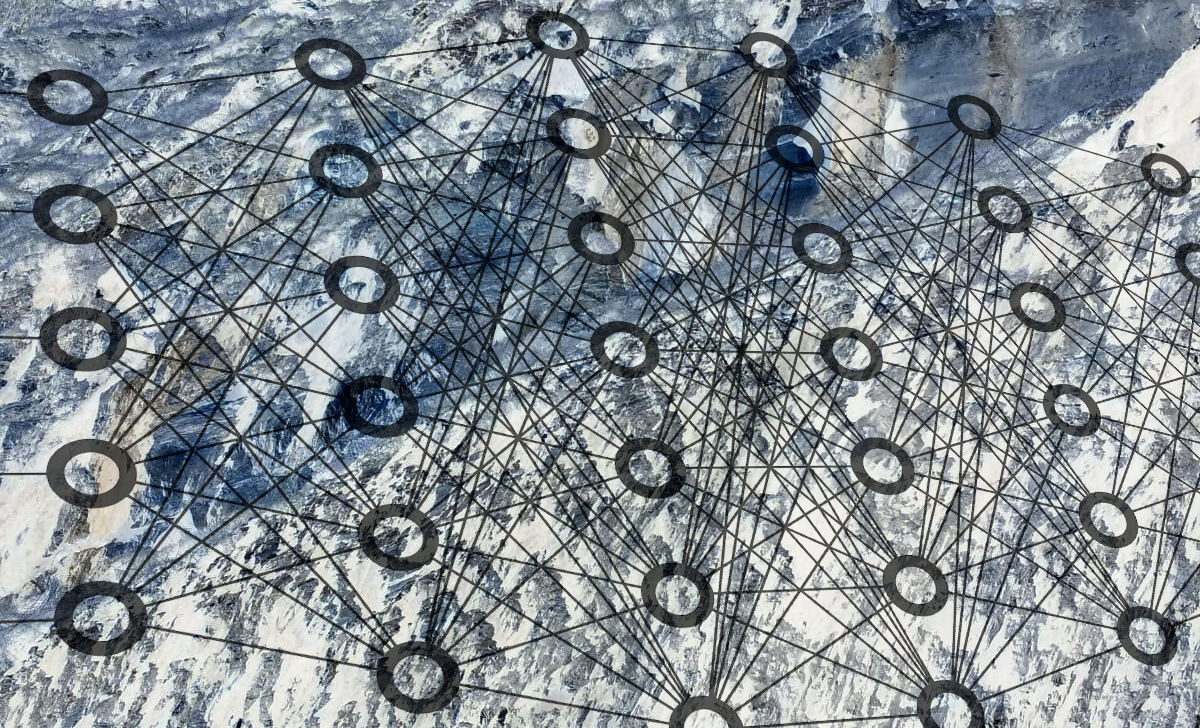
\includegraphics[height=\paperheight,width=\paperwidth]{frames/auxiliar/title_img/prueba.png}};}

\begin{frame}[plain]
\begin{variableblock}{}{bg=myblue,fg=white}{bg=green,fg=red}
\begin{center}
\textbf{Database Generation for Borehole Inversion Problems}
\end{center}
\end{variableblock}
\end{frame}
}
%%%%%%%%%%%%%%%%%%%%%%%%%%%%%%%%%%%%%%%%%%%%%%%%%%%%%%%%%%%%%%%%%%%
%\begin{frame}[t]{Database for Inversion}
Deep Learning methods are fast, but they \textbf{require a massive training dataset}.
\vspace{0.2cm}

We need to solve Maxwell's equations. \textcolor{red}{3D simulations are expensive}. Reduce dimensionality using Fourier or Hankel transforms. (So called 1.5D and 2.5D formulations).
\vspace{0.2cm}

\visible<2-3>{Methods to solve PDEs: FEM and IGA.
\begin{itemize}
\item IGA provides smoother solutions.
\item \textcolor{red}{IGA increases cost of LU factorization}
\end{itemize}
\vspace{0.2cm}

\textbf{rIGA} decreases the cost of LU factorization.
\vspace{0.2cm}

\begin{thebibliography}{1}
\bibitem{Dani} D. Garcia et al. The value of continuity: Refined isogeometric analysis and fast direct solvers. Computer Methods in Applied Mechanics and Engineering, 316: 586–605, 2017.
\end{thebibliography}
}
\vspace{0.2cm}

\visible<3>{In this Section, \textbf{we use rIGA methods to generate a database for DL inversion.}}
\end{frame}


\begin{frame}[t]{rIGA Database Generation}
\begin{columns}
    \begin{column}{0.35\textwidth}
    \begin{figure}[!h]
	\centering
	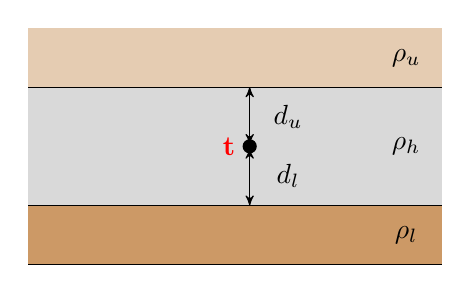
\begin{tikzpicture}[scale=1.5]
\draw (0,0) rectangle (3.5,2);

\fill[white!20!brown] (0,0) rectangle (3.5,0.5);
\fill[white!70!gray] (0,0.5) rectangle (3.5,1.5);
\fill[white!60!brown] (0,1.5) rectangle (3.5,2);


%\draw[red, line width=0.5 mm] (0.75,1.5) .. controls (1.15,1.1) .. (1.85,1) node (n1) at (0.85,1.6) {$\mathbf{t}$};
\draw[black, line width=0.1 mm] (0,0.5) -- (3.5,0.5);
\draw[black, line width=0.1 mm] (0,1.5) -- (3.5,1.5);

\fill[black] (1.875,1) circle (0.06cm);
\node (d_u) at (1.7,1) {\textcolor{red}{$\textbf{t}$}};
\draw[<->] (1.875,1.02) -- (1.875,1.5);
\node (d_u) at (2.2,1.25) {$d_u$}; 
\draw[<->] (1.875,0.98) -- (1.875,.5);
\node (d_u) at (2.2,0.75) {$d_l$};
\node (rho) at (3.2,1.75) {$\rho_u$};
\node (rho) at (3.2,0.25) {$\rho_l$};
\node (rho) at (3.2,1) {$\rho_h$};
\end{tikzpicture}

	\label{fig:param}
	\end{figure}
    \end{column}
    \begin{column}{0.5\textwidth}
        {\footnotesize $\rho_u \in [1,10^2] \Omega \cdot m$: Upper layer resistivity}\\
        \vspace{0.3cm}
        {\footnotesize $\rho_h \in [1,10^2] \Omega \cdot m$: Central layer resistivity}\\
        \vspace{0.3cm}
        {\footnotesize $\rho_l \in [1,10^2] \Omega \cdot m$: Lower layer resistivity}\\
        \vspace{0.3cm}
        {\footnotesize $d_u \in [10^{-2},10] m$: Vertical distance to upper layer}\\
        \vspace{0.3cm}
        {\footnotesize $d_l \in [10^{-2},10] m$: Vertical distance to lower layer}
    \end{column}
\end{columns}
\vspace{0.2cm}

\begin{itemize}
\item Generate $100.000$ samples and compute their measurements.
\vspace{0.2cm}
\item We need $\simeq 56$h to generate the database.
\end{itemize}

\begin{thebibliography}{2}
\bibitem{Ali} A. Hashemian, D. Garcia, J. A. Rivera and D. Pardo. Massive database generation for 2.5 D borehole electromagnetic measurements using refined isogeometric analysis. Computers \& Geosciences 155, 104808, 2021.
\end{thebibliography}
\end{frame}


%\begin{frame}{PREGUNTAS y COMENTARIOS}
%No se nada de IGA. Por eso no me atrevo a poner nada mas. Y si me preguntan algo de esto quiero saber como contestar. Vamos, quiero saber que frase decir para quedar bien.
%\vspace{0.5cm}
%
%La verdad que no se como poner los resultados. O mejor dicho, que mas poner.
%\vspace{0.5cm}
%
%Tengo varias preguntas para hacerte sobre este topic. Quiero intentar al menos llevar un par de conceptos preparados.
%\end{frame}




%\begin{frame}{Isogeometric Analysis}

%Una slide donde explique que es rIGA de una manera muy facil (tengo que entenderlo yo) y sus ventajas
%
%Que es lo que yo he contribuido en este trabajo? En la parte de resolver el problema inverso? A mi me daban unos datos y yo les daba otros. Creo que em daban att/ph y les daba las resistividades????? Lo que hacia era ejecutar una tabla
%
%Poner directamente los resultados obtenidos. Pondria los dos graficos de la generacion de la base de datos y ya. Tal vez tiempos y asi.
%
%POR QUE HAY UNA CORRELACION LINEAL ENTRE ATENUATION Y PHASE????????

%\end{frame}


%\end{section}
%%%%%%%%%%%%%%%%%%%%%%%%%%%%%%%%%%
%%%%%%%%%%%%%%%%%%%%%%%%%%%%%%%%%%
%\begin{section}{Solving Forward Problems (PDEs) with Neural Networks}
%%%%%%%%%
{
\usebackgroundtemplate{\tikz\node[opacity=0.1,inner sep=0] {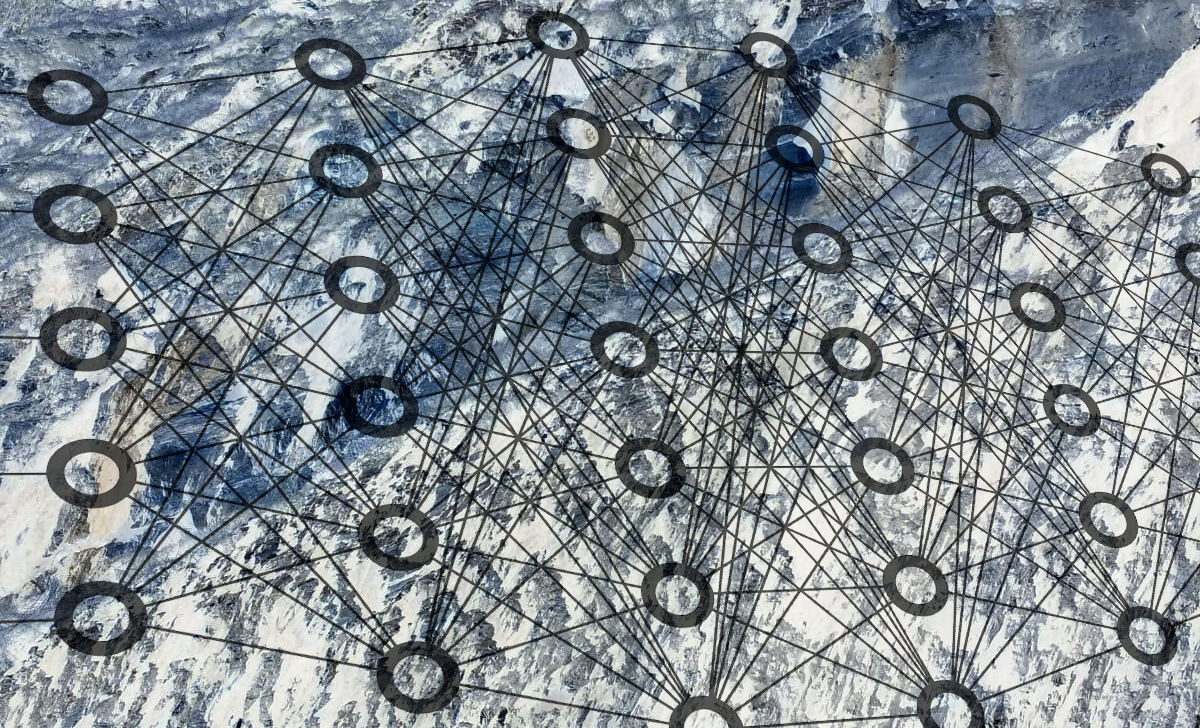
\includegraphics[height=\paperheight,width=\paperwidth]{frames/auxiliar/title_img/prueba.png}};}

\begin{frame}[plain]
\begin{variableblock}{}{bg=myblue,fg=white}{bg=green,fg=red}
\begin{center}
\textbf{Solving Forward Problems (PDEs) with Neural Networks}
\end{center}
\end{variableblock}
\end{frame}
}
%%%%%%%%%%%%%%%%%%%%%%%%%%%%%%%%%%%%%%%%%%%%%%%%%%%%%%%%%%%%%%%%%%%
%\begin{frame}[t]{Deep Neural Networks for Solving PDEs}
\visible<1-3>{\textbf{Objective:} Generate the database for DL inversion faster than with traditional methods.}
\vspace{0.2cm}

\visible<2-3>{\textbf{Main goal:} Solve a \textcolor{blue}{parametric} PDE using NNs.
\vspace{0.2cm}

$
\left\{
\begin{array}{rrcl}
-\nabla \cdot (\textcolor{blue}{\sigma} \nabla u) & = & f & \; \text{in} \; \Omega, \\ 
u & = & 0 & \; \text{on} \; \Gamma_D,\\  
(\textcolor{blue}{\sigma}\nabla u) \cdot \bs{n}  & = & g & \; \text{on} \; \Gamma_N.
\end{array}
\right.
$
}
\vspace{0.2cm}

\visible<3>{\textbf{First step:} Approximate a non-parametric ($\textcolor{blue}{\sigma}:= 1$) PDE solution by a NN.
%\begin{equation*}
%u \approx u_{NN}.
%\end{equation*}
\vspace{0.2cm}

$
\left\{
\begin{array}{rrcl}
-\bigtriangleup u & = & f & \; \text{in} \; \Omega, \\ 
u & = & 0 & \; \text{on} \; \Gamma_D,\\  
\nabla u \cdot \bs{n}  & = & g & \; \text{on} \; \Gamma_N.
\end{array}
\right.
$

\begin{thebibliography}{1}
\bibitem{pinn} {\small J. A. Rivera, J. M. Taylor, A. J. Omella, and D. Pardo. On quadrature rules for solving Partial Differential Equations using Neural Networks. Computer Methods in Applied Mechanics and Engineering 393, 114710, 2022.}
\end{thebibliography}
}
\end{frame}


\begin{frame}[t]{Deep Neural Networks for Solving PDEs}
\textbf{Physics-Informed Neural Networks (PINNs)}

Monte Carlo integration
\begin{thebibliography}{2}
\bibitem{pinn} {\small Z. Mao, A. D. Jagtap, and G. E. Karniadakis. Physics-informed neural networks for high-speed flows. Computer Methods in Applied Mechanics and Engineering, 360:112789, 2020.}
\end{thebibliography}
Gaussian quadrature rule

\textit{"there is no proper quadrature rule in the literature developed for integrals of DNNs"}
\begin{thebibliography}{2}
\bibitem{vpinn} {\small E. Kharazmi, Z. Zang, and G. E. Karniadakis. VPINNs: Variational Physics-Informed Neural Networks For Solving Partial Differential Equations, \textit{Arxiv}, 2019.}
\end{thebibliography}

\textbf{Deep Least Square}

Adaptive integration.
\begin{thebibliography}{3}
\bibitem{DLS} {\small Z. Cai, J. Chen, M. Liu, and X. Liu. Deep least-squares methods: An unsupervised learning-based numerical method for solving elliptic PDEs.
Journal of Computational Physics, 420:109707, 2020.}
\end{thebibliography}
\end{frame}




\begin{frame} {Deep Ritz Method (DRM)}
\vspace{-0.2cm}
\begin{thebibliography}{1}
\bibitem{Ritz}E, W., Yu, B.: The Deep Ritz method: A Deep Learning-Based Numerical Algorithm for Solving Variational Problems. Communications in Mathematics and Statistics \textbf{6}, 1--12 (2018)
\end{thebibliography}
\vspace{0.3cm}

Minimization of the total energy:

\begin{equation*}
 \mathcal{L}_{Ritz}  := \frac{1}{2} \int_{\Omega} (\nabla u )^2 - \int_{\Omega} f \, u - \int_{\Gamma_N }g \, u
\end{equation*}

\begin{itemize}
%\item Requires a symmetric and positive definite bilinear form.
\item We will denote $\mathcal{L}_{Ritz}$ as $\mathcal{L}_{\mathcal{R}}$
\item Standard inner products:
\begin{equation*}
(u,v) = \int_{\Omega} u \, v
\end{equation*}
\end{itemize}
\end{frame}



%%%%%%%%%
{
\usebackgroundtemplate{\tikz\node[opacity=0.1,inner sep=0] {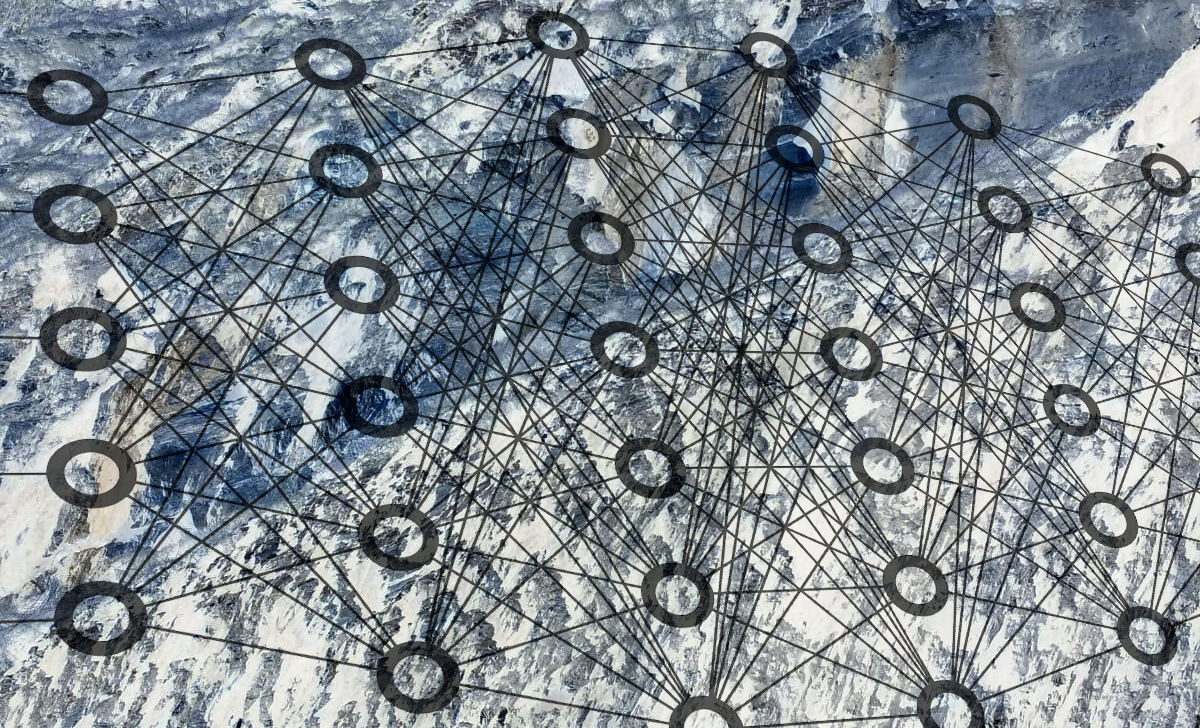
\includegraphics[height=\paperheight,width=\paperwidth]{frames/auxiliar/title_img/prueba.png}};}

\begin{frame}[plain]
\begin{variableblock}{}{bg=myblue,fg=white}{bg=green,fg=red}
\begin{center}
\textbf{Quadrature Problems when Solving PDEs with DNNs}
\end{center}
\end{variableblock}
\end{frame}
}
%%%%%%%%%%%%%%%%%%%%%%%%%%%%%%%%%%%%%%%%%%%%%%%%%%%%%%%%%%%%%%%%%%%
%\begin{frame}[t]{Numerical example}
\begin{columns}[T] % align columns
\begin{column}{.48\textwidth}
We solve the following PDE problem:
\begin{subequations}
\begin{empheq}[left= \empheqlbrace]{align}
    \; -\nabla \cdot ( \nabla u) & = 0.21x^{-1.3} &  x \in (0,10), \notag \\
    u & = 0 &  x =0, \notag \\
    ( \nabla u) \cdot \bf{n}  & = 0.7x^{-0.3}  &  x=10. \notag 
\end{empheq}
\end{subequations}

Exact solution: $u_{exact}=x^{0.7}$.
\vspace{0.5cm}

Loss value of the exact solution: $\mathcal{L}_{\mathcal{R}}(u)=-1.54$.

\end{column}%

\hfill%

\begin{column}{.48\textwidth}
\begin{figure}[!htp]
\centering
 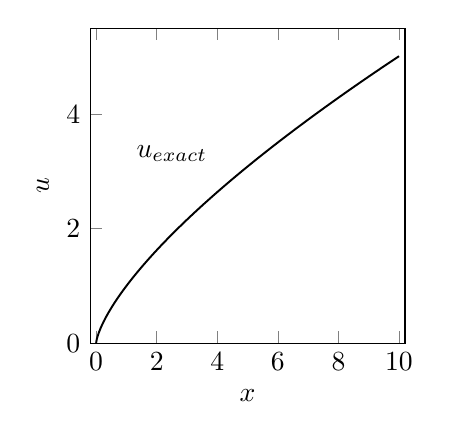
\begin{tikzpicture}
\begin{axis}[scale only axis, xlabel = $x$, ylabel = $u$, ytick pos=left, y label style={at={(-0.1,0.5)}}, legend style= {at={(0.6,0.98)},draw=none,fill=none,nodes={scale=0.8, transform shape}}, legend cell align={left}, height=4cm, width=4cm, xmin=-0.2, ymin=0, xmax=10.2, ymax=5.5,samples=1000]
\addlegendimage{only marks, mark=-, color=black} 
\addplot [black, line width=0.7pt,domain=0:10] {x^0.7};
%\addlegendentry{Exact solution}
% Legend
\node[anchor = south] at (2.5,3){\textcolor{black}{$u_{exact}$}};
\end{axis}
\end{tikzpicture}

%\caption*{Loss evolution.}
	\label{fig:ritz_exact}
 \end{figure}
\end{column}%
\end{columns}
\end{frame}


\begin{frame}[t]{Loss function}
Let $\{ K_i \}_{i=1}^{n}$ be a partition of $\Omega$ and $\{ L_j \}_{j=1}^{m}$ a partition of $\Gamma_N$.

\begin{equation}
\mathcal{L}_{\mathcal{R}}(u) = \frac{1}{2} \sum_{i=1}^{n} ( \nabla u,\nabla u)_{K_i} - \sum_{i=1}^{n} (f,u)_{K_i} - \sum_{j=1}^{m} (g,u)_{L_j}.
\notag
\end{equation}

\textbf{Gradient computation:}
\vspace{0.15cm}

\begin{itemize}
\item Automatic differentiation.
\end{itemize}

\vspace{0.25cm}
\textbf{Gaussian Quadrature:} Three Gaussian points.
\vspace{0.15cm}
\begin{figure}[!htp]
\centering
	\begin{tikzpicture}
\draw (0,0) -- (8,0);
\foreach \Point in {(0,0), (8,0)}{\node at \Point {\textbullet};}
\foreach \Point in {(1,0), (4,0), (7,0)}{\node[blue] at \Point {\textbullet};}
%\node at (9.5,0) {\textup{Training set}};
\node[blue] at (1,0.3) {$q_1$};
\node[blue] at (4,0.3) {$q_2$};
\node[blue] at (7,0.3) {$q_3$};
\node at (0,-0.25) {$x_i$};
\node at (8,-0.25) {$x_{i+1}$};
\end{tikzpicture}
	\label{fig:partition}
\end{figure} 
\end{frame}


\begin{frame}{Architecture Sketch}
\def\layersep{1.5cm}
\centering

%\begin{tikzpicture}[x=1cm,y=0.8cm]
%%\draw[very thin, rounded corners=5pt,fill=orange!30!white ,opacity=0.5] (4.0,0.2) rectangle (10,1.3);
%\node at (7.0,0.75){\Large $u \approx u_{NN} := \underset{\theta \in V}{\textup{ arg min }} \mathcal{L}_{(\cdot)}(\theta)$};
%\end{tikzpicture}
%
%\vspace{0.4cm}

\begin{tikzpicture}[shorten >=1pt,->,draw=black!50, node distance=\layersep]
    \tikzstyle{every pin edge}=[<-,shorten <=1pt]
    \tikzstyle{neuron}=[circle,fill=black!25,minimum size=20pt,inner sep=0pt]
    \tikzstyle{neuron2}=[circle,fill=black!25,minimum size=15pt,inner sep=0pt]
    \tikzstyle{input lay}=[rectangle,fill=green!50,minimum width=30pt, minimum height=100pt,inner sep=0pt]
%    \tikzstyle{input neuron}=[neuron, fill=green!50];
	\tikzstyle{hidden neuron}=[neuron2, fill=blue!50];
	\tikzstyle{ghost neuron}=[neuron, fill=gray!40!white, , opacity=1];
    \tikzstyle{output neuron}=[neuron, fill=red!50];
    \tikzstyle{output lay}=[rectangle,fill=red!50,minimum width=30pt, minimum height=100pt,inner sep=0pt]
    
	\tikzstyle{multi neuron}=[neuron, fill=purple!50];
    \tikzstyle{multi lay}=[rectangle,fill=purple!50,minimum width=30pt, minimum height=100pt,inner sep=0pt]	
	
	
	\tikzstyle{final neuron}=[neuron, fill=brown!50];
	
    \tikzstyle{annot} = [text width=4em, text centered]
	\tikzstyle{annot final} = [text width=10em, text centered]


\draw[very thin, rounded corners=5pt,fill=gray!40!white ,opacity=1] (0,1.5) rectangle (6,-4);
\draw[very thin, rounded corners=5pt,fill=gray!30!white ,opacity=1] (0.3,1.8) rectangle (4.0,1.2);
\node [anchor = west] at (0.3,1.5){Deep Neural Network};

    % Draw the input layer nodes
    \foreach \name / \y in {1}
        \node[input lay] (I-\name) at (0,-1) {$x$};

%    % Draw the hidden layer nodes
%    \foreach \name / \y in {1,...,3}
%        \path[yshift=1.5cm]
%            node[hidden neuron, xshift=0.5cm] (H-\name) at (\layersep,-\y cm) {};
	
\path[yshift=1.5cm] node[hidden neuron, xshift=0.5cm] (H1_1) at (\layersep,-1 cm) {};	
\path[yshift=1.5cm] node[hidden neuron, xshift=0.5cm] (H1_2) at (\layersep,-2 cm) {};
\path[yshift=1.5cm] node[ghost neuron, xshift=0.5cm] (Hghost1) at (\layersep,-3 cm) {$\vdots$};
\path[yshift=1.5cm] node[hidden neuron, xshift=0.5cm] (H1_3) at (\layersep,-4 cm) {};
	
\path[yshift=1.5cm] node[hidden neuron, xshift=0.0cm] (H2_1) at (2.5*\layersep,-1 cm) {};	
\path[yshift=1.5cm] node[hidden neuron, xshift=0.0cm] (H2_2) at (2.5*\layersep,-2 cm) {};
\path[yshift=1.5cm] node[ghost neuron, xshift=0.0cm] (Hghost2) at (2.5*\layersep,-3 cm) {$\vdots$};
\path[yshift=1.5cm] node[hidden neuron, xshift=0.0cm] (H2_3) at (2.5*\layersep,-4 cm) {};

\path[yshift=1.5cm] node[ghost neuron, xshift=0.2cm] (Hghosta) at (1.75*\layersep,-1 cm) {$\hdots$};
\path[yshift=1.5cm] node[ghost neuron, xshift=0.2cm] (Hghostb) at (1.75*\layersep,-2 cm) {$\hdots$};
\path[yshift=1.5cm] node[ghost neuron, xshift=0.2cm] (Hghostc) at (1.75*\layersep,-4 cm) {$\hdots$};

%    % Draw the output layer node
    \node[output lay, right of=Hghost2, yshift=0.5cm, xshift=0.5cm] (O) {$\tilde{u}_{NN, \theta}$};
    
    % Multiply BC function
	\node[multi lay, right of=O,  xshift=1.5cm] (M) {$u_{NN, \theta}$};
%	\node[multi lay, right of=Hghost2, yshift=0.5cm, xshift=0.5cm] (M) {$u_{NN}$};
	
	% Final output, after Loss
	\node[final neuron, right of=M, xshift=1.8cm] (F) {$\mathcal{L}(u_{NN, \theta})$};

    % Connect every node in the input layer with every node in the
    % hidden layer.
    \foreach \source in {1}
        \foreach \dest in {1,...,3}
            \path (I-\source) edge (H1_\dest);

    % Connect every node in the hidden layer with the output layer
    \foreach \source in {1,...,3}
        \path (H2_\source) edge (O);
        
%	% Connect output kayer and multiply layer
	\path[every node/.style={anchor=south}] (O) edge node {Impose BC} (M);
	
	% Connect output kayer and multiply layer
	\path[every node/.style={anchor=south}] (M) edge node {Define loss} (F);

    % Annotate the layers
%    \node[text width=10em, text centered, ,above of=Hghosta, node distance=0.7cm] {Hidden layers};
    \node (texto)[text width=15.5em, text centered, ,below of=Hghostc, node distance=1cm] {Trainable parameters: \\ $\theta:= \{$weights, biases$\}$};
    
%    \node[text width=6.5em, text centered, ,right of=texto, node distance=4.5cm] {Non-trainable layer};
%    \node[text width=6.5em, text centered, ,right of=texto, node distance=7.5cm] {Non-trainable layer};
    
%    \node[text width=4em, text centered, ,above of=I-1, node distance=2.cm] {\footnotesize INPUT};
%    \node[text width=4em, text centered, ,above of=F, node distance=1.cm] {\footnotesize OUTPUT};
\end{tikzpicture}

\vspace{0.2cm}
\small To impose the homogeneous Dirichlet BC, we define:

$u_{NN, \theta} := \phi(x) \cdot \tilde{u}_{NN, \theta}$, where 
$ \left\{
\begin{array}{l}
\phi(x) = 0,  \quad \text{if} \; x \in \Gamma_D,\\ 
\phi(x) \neq 0, \quad \text{if} \; x \not \in \Gamma_D.
\end{array}
\right.$
\end{frame}


\begin{frame}[t]{Numerical example}
\visible<1-2>{Loss evolution of the DL method optimization process.

\begin{figure}[!htp]
\centering
 \begin{tikzpicture}
%https://tex.stackexchange.com/questions/451704/tikz-position-of-an-imported-image
  \node[anchor=south west,inner sep=0] (image) at (0,0) {\begin{tikzpicture}
\begin{axis}[scale only axis, xlabel = $Epoch$, ylabel = $Loss$, ytick pos=left, y label style={at={(-0.12,0.5)}}, legend style= {at={(0.65,0.35)},draw=none,fill=none,nodes={scale=0.8, transform shape}}, legend cell align={left}, height=4cm, width=12cm, xmin=0.95, ymin=-15, xmax=45000, ymax=12, ytick = {8,-1.54,-15}, xmode=log, xticklabel style={yshift=-3pt}, yticklabel style={xshift=-3pt}]
\addplot [black, dashed, line width=0.7pt,domain=0.99999:39900] {-1.54};
%\addlegendentry{Loss of exact solution}
\addplot[line width=0.8pt,color=red] %
	table[x=epoch ,y=loss]{Diapos/PDEs_with_NN/Figures/Quadrature_problem//Data//loss_Ritz_normal_treshold.csv};
%\addlegendentry{Loss of NN approximation};

\end{axis}
\end{tikzpicture}
};
  \begin{scope}[x={(image.south east)},y={(image.north west)}]
  \draw[<-] (0.3,0.55) -- (0.35,0.45) node[below right] {\textcolor{black}{$\mathcal{L}_{\mathcal{R}}(u_{exact})$}};
  \draw[<-, color=red] (0.35,0.7) -- (0.6,0.85) node[above right] {\textcolor{red}{$\mathcal{L}_{\mathcal{R}}(u_{NN})$}};
  \end{scope}
\end{tikzpicture}

%\caption*{Loss evolution.}
	\label{fig:ritz_normal_loss}
 \end{figure}}
 
\visible<2-2>{
\begin{center}
\textcolor{red}{We obtain a better loss than the optimum!}
\end{center}
}

\end{frame}


\begin{frame}[t]{Numerical example}
Mesh with four elements. Three Gauss points per element.
\vspace{0.5cm}

\begin{minipage}{.4\textwidth}
\begin{figure}[!htp]
\centering
 \begin{tikzpicture}
\begin{axis}[scale only axis, xlabel = $x$, ylabel = $u$, ytick pos=left, y label style={at={(-0.1,0.5)}}, legend style= {at={(0.6,0.98)},draw=none,fill=none,nodes={scale=0.8, transform shape}}, legend cell align={left}, height=4cm, width=4cm, xmin=-0.2, ymin=0, xmax=10.2, ymax=50]
\addlegendimage{only marks, mark=-, color=black} 
\addlegendimage{only marks, mark=-, color=red}
\addplot [black, line width=0.7pt,domain=0:10] {x^0.7};
%\addlegendentry{Exact solution}
\addplot[line width=0.5pt,color=red] %
	table[x=x ,y=u_pred]{Diapos/PDEs_with_NN/Figures/Quadrature_problem//Data//data_Ritz_normal.csv};
%\addlegendentry{Gauss/AD};
\addplot[densely dashed, blue] coordinates {
      (0.01, 18)
      (2.5, 18)
      (2.5,  48)
      (0.01, 48)
      (0.01, 18)
    };

% Legend
\node[anchor = south] (Ua)at (6,32){\textcolor{red}{$u_{NN}$}};
\node[anchor = south] at (6,6){\textcolor{black}{$u_{exact}$}};

\end{axis}
\end{tikzpicture}

\caption*{Exact and approximated solutions}
	\label{fig:ritz_exact}
 \end{figure}
\end{minipage}%
\begin{minipage}{.2\textwidth}
\center
\vspace{-2.5cm}
\tikzfancyarrow{Zoom}
\end{minipage}%
\begin{minipage}{.4\textwidth}
\begin{figure}[!htp]
\centering
 \begin{tikzpicture}
\begin{axis}[scale only axis, xlabel = $x$, ylabel = $u$, ytick pos=left, y label style={at={(-0.1,0.5)}}, height=4cm, width=4cm, xmin=0, ymin=18, xmax=2.5, ymax=50]
%\addlegendimage{only marks, mark=-, color=black} 
%\addlegendimage{only marks, mark=-, color=red}
\addplot [black, line width=0.7pt,domain=0:10] {x^0.7};
%\addlegendentry{Exact solution}
\addplot[line width=0.5pt,color=red] %
	table[x=x ,y=u_pred]{Diapos/PDEs_with_NN/Figures/Quadrature_problem//Data//data_Ritz_normal.csv};
\addplot[only marks, blue, mark size=1.25] coordinates {
      (0.28175, 19)
      (1.25, 46.27)
      (2.21825, 36.05)
    };
    


\node(G)[anchor = north, text width=1.0] at (axis cs: 1.5,30)
 {\textcolor{blue}{Gauss points}};
\node(G_aux1)[anchor = north, text width=1.0] at (axis cs: 1.65,31) {};
\node(G_aux2)[anchor = north, text width=1.0] at (axis cs: 2,31) {};
    

\node (G1) at (axis cs: 0.28175, 19){};
\node (G2) at (axis cs: 1.25, 46.27){};
\node (G3) at (axis cs: 2.21825, 36.05){};


\path[->, blue] (G) edge (G1);
\path[->, blue] (G_aux1) edge (G2);
\path[->, blue] (G_aux2) edge (G3);
%\addlegendentry{Gauss/AD};
\end{axis}
\end{tikzpicture}
\caption*{Zoom on the approximated solution}
	\label{fig:ritz_exact}
 \end{figure}
\end{minipage}%
\end{frame}


\begin{frame}[t]{Numerical example}
\begin{equation}
\notag
\mathcal{L}_{\mathcal{R}}(u_{NN}) = \frac{1}{2} \underbrace{( \nabla u_{NN},\nabla u_{NN})}_{ \sum_{q_i} \omega_i (\nabla u_{NN})^2 \approx 0} - \underbrace{(f,u_{NN})}_{\infty} - (g,u_{NN})_{\Gamma_N} \simeq - \infty
\notag
\end{equation}

\begin{figure}[!htp]
\centering
	%\subcaptionbox{Approximated solution at interval $[0,2.5]$}
	{\begin{tikzpicture}
\begin{axis}[scale only axis, xlabel = $x$, ylabel = $u$, ytick pos=left, y label style={at={(-0.1,0.5)}}, height=4cm, width=4cm, xmin=0, ymin=18, xmax=2.5, ymax=50]
%\addlegendimage{only marks, mark=-, color=black} 
%\addlegendimage{only marks, mark=-, color=red}
\addplot [black, line width=0.7pt,domain=0:10] {x^0.7};
%\addlegendentry{Exact solution}
\addplot[line width=0.5pt,color=red] %
	table[x=x ,y=u_pred]{Diapos/PDEs_with_NN/Figures/Quadrature_problem//Data//data_Ritz_normal.csv};
\addplot[only marks, blue, mark size=1.25] coordinates {
      (0.28175, 19)
      (1.25, 46.27)
      (2.21825, 36.05)
    };
    


\node(G)[anchor = north, text width=1.0] at (axis cs: 1.5,30)
 {\textcolor{blue}{Gauss points}};
\node(G_aux1)[anchor = north, text width=1.0] at (axis cs: 1.65,31) {};
\node(G_aux2)[anchor = north, text width=1.0] at (axis cs: 2,31) {};
    

\node (G1) at (axis cs: 0.28175, 19){};
\node (G2) at (axis cs: 1.25, 46.27){};
\node (G3) at (axis cs: 2.21825, 36.05){};

\draw[] (G1) node[above, blue] {\footnotesize $q_1$};
\draw[] (G2) node[above, blue] {\footnotesize $q_2$};
\draw[] (G3) node[above, blue] {\footnotesize $q_3$};


\path[->, blue] (G) edge (G1);
\path[->, blue] (G_aux1) edge (G2);
\path[->, blue] (G_aux2) edge (G3);
%\addlegendentry{Gauss/AD};
\end{axis}
\end{tikzpicture}} 
	\hspace{0.5cm}
	%\subcaptionbox{Loss evolution}
	{\begin{tikzpicture}
\begin{axis}[scale only axis, xlabel = $Epoch$, ylabel = $Loss$, ytick pos=left, y label style={at={(-0.25,0.5)}}, legend style= {at={(0.8,0.4)},draw=none,fill=none,nodes={scale=0.7, transform shape}}, legend cell align={left}, height=4cm, width=6cm, xmin=0.95, ymin=-15, xmax=45000, ymax=12, ytick = {8,-1.54,-15}, xmode=log]
\addplot [black, dashed, line width=0.7pt,domain=0.99999:39900] {-1.54};
%\addlegendentry{Loss of exact solution}
\addplot[line width=0.8pt,color=red] %
	table[x=epoch ,y=loss]{Diapos/PDEs_with_NN/Figures/Quadrature_problem//Data//loss_Ritz_normal_treshold.csv};
%\addlegendentry{Loss of NN approximation.};

% Legend
%\node[anchor = south] (Ua)at (6,32){\textcolor{red}{$u_{approx}$}};
%\node[anchor = south] at (6,6){\textcolor{black}{$u_{exact}$}};

\end{axis}
\end{tikzpicture}
}
\end{figure} 
\end{frame}


%%%%%%%%%
{
\usebackgroundtemplate{\tikz\node[opacity=0.1,inner sep=0] {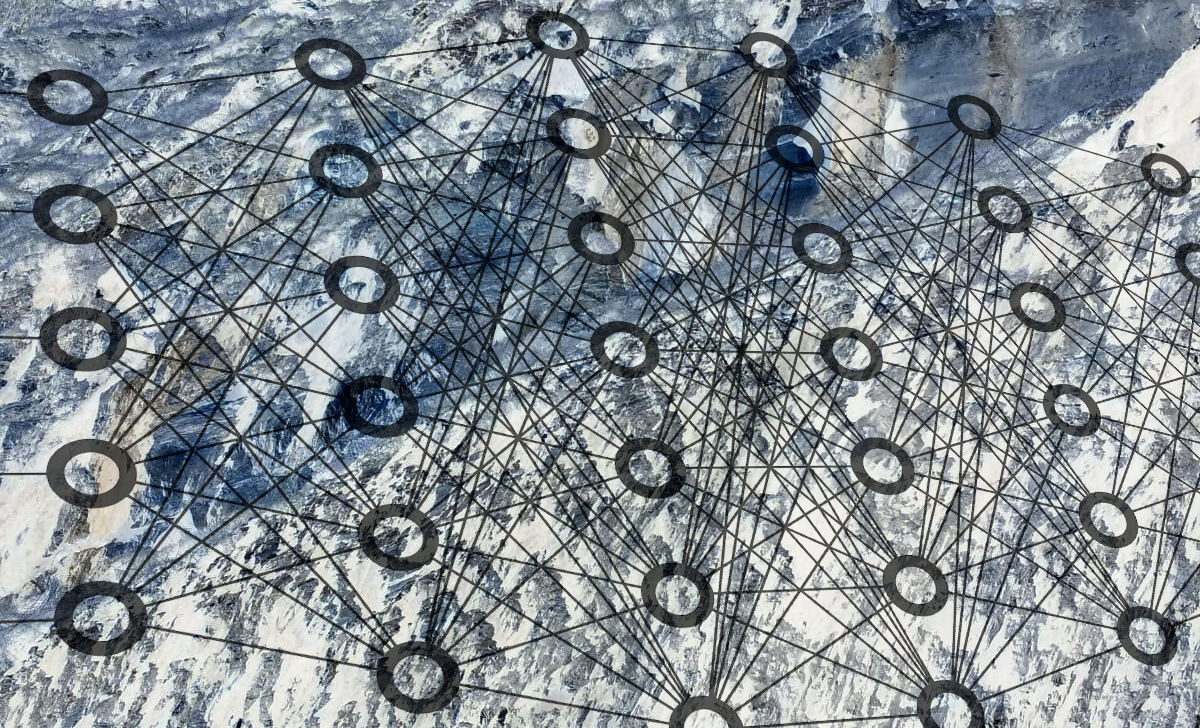
\includegraphics[height=\paperheight,width=\paperwidth]{frames/auxiliar/title_img/prueba.png}};}

\begin{frame}[plain]
\begin{variableblock}{}{bg=myblue,fg=white}{bg=green,fg=red}
\begin{center}
\textbf{Alternatives to Overcome Quadrature Problems}
\end{center}
\end{variableblock}
\end{frame}
}
%%%%%%%%%%%%%%%%%%%%%%%%%%%%%%%%%%%%%%%%%%%%%%%%%%%%%%%%%%%%%%%%%%%
%\begin{frame}{Monte Carlo integration}
\begin{center}
$
\ds \int_a^b f(x) dx \approx \frac{b-a}{N} \sum_{i=1}^N f(X_i), \;
$
where $X \sim Uniform(a,b)$
\end{center}

\begin{itemize}
\item[\tickYes] Convergence rate independent of the dimension: $\mathcal{O}(N^{-1/2})$
\item[\tickNo] Slow convergence in low dimensions (1D, 2D, 3D)
\item[\tickYes] Appropriate for high dimensions
\item[\tickYes] Mesh-free method
\item[\tickYes] Allows the use of autodiff to compute $\nabla u$
\item[\tickYes] Easy to implement
\item[\tickYes] Exploit the use of minibatches and GPUs
\end{itemize}
\end{frame}


\begin{frame}{Explainability of the NN: Regularization methods}
\centering

\begin{itemize}
\item We  minimise the loss:
$$\mathcal{L}_{total} = \mathcal{L}_{Ritz}+R.$$
\vspace{0.2cm}

\item Using arguments similar to (Mishra \textit{et al.}, 2020), we define $R$ for a simple NN as:

\begin{equation*}
R\left(\theta, u_{NN}(x_i), \dfrac{\partial^{n}u_{NN}(x_i) }{\partial x^{n}} \right).
\end{equation*}


\vspace{0.2cm}
\item $R$ acts as a regularizer, penalising poor quadrature via the loss. 
%\vspace{0.2cm}
%\item $\mathcal{R}\sim \frac{1}{N}$, so for $N$ large, the ``bias" from $\mathcal{R}$ vanishes.
%

\vspace{0.5cm}

%\beamertemplatebookbibitems
\begin{thebibliography}{1}
%\bibitem{Author1990}A. Author. \newblock\emph{Handbook of Everything}.\newblock
%Some Press, 1990.\beamertemplatearticlebibitems
\bibitem{Mishra}Mishra, S., Molinaro, R.: Estimates on the generalization error of physics informed neural
networks (PINNs) for approximating PDEs. ArXiv:2006.16144 (2020).
\end{thebibliography}
\end{itemize}
\end{frame}


\begin{frame}{Explainability of the NN: Regularization methods}
\vspace{0.25cm}
\begin{itemize}
\item[\tickYes]The loss prohibits overfitting
\vspace{0.15cm}

\item[\tickYes] We have {\it a posteriori} estimation of quadrature error
\vspace{0.15cm}

\item[\tickYes] $R$ is computationally cheap to evaluate
\vspace{0.15cm}
%
%\item[\tickNo] If $N$ is small, the problem is drastically changed by $R$
%\vspace{0.15cm}

\item[\tickNo] Finding an expression for $R$ is difficult and problem dependent
\vspace{0.15cm}

\item[\tickNo] Only valid for regular integrands
\end{itemize}
\end{frame}


\begin{frame}{Adaptive Integration}
\only<1-1>{
\centering
\begin{columns}
\begin{column}{0.7\textwidth}
	\begin{figure}[!htp]
		\begin{tikzpicture}
% TRAIN
\node at (1,1) {};
\node at (1,-4) {};

\draw[<->, dashed] (0,0.5) -- (2,0.5);
\node at (1,0.75) {$h$};
\draw (0,0) -- (8,0);
\foreach \Point in {(0,0), (2,0), (4,0), (6,0), (8,0)}{\node at \Point {\textbullet};}
\node at (0,-0.25) {$a$};
\node at (8,-0.25) {$b$};


% VALIDATION
\draw[<->, dashed] (0,-3.5) -- (1,-3.5);
\node at (0.5,-3.75) {$h/2$};

\draw (0,-3) -- (8,-3);
\foreach \Point in {(0,-3), (2,-3), (4,-3), (6,-3), (8,-3)}{\node at \Point {\textbullet};}
\foreach \Point in {(1,-3), (3,-3), (5,-3), (7,-3)}{\node[blue] at \Point {\textbullet};}
\node at (0,-3.25) {$a$};
\node at (8,-3.25) {$b$};

\end{tikzpicture}
		\label{fig:adaptive_1}
 	\end{figure}
\end{column}

\begin{column}{0.3\textwidth}
Training set

\vspace{2.5cm}

Validation set
\end{column}
\end{columns}
 }

\only<2-2>{
\centering
\begin{columns}
\begin{column}{0.7\textwidth}
	\begin{figure}[!htp]
		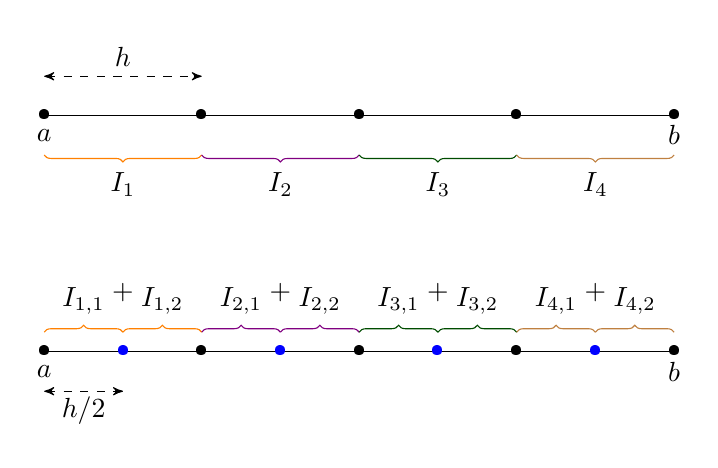
\begin{tikzpicture}
\node at (1,1) {};
\node at (1,-4) {};
% TRAIN
\draw[<->, dashed] (0,0.5) -- (2,0.5);
\node at (1,0.75) {$h$};
\draw (0,0) -- (8,0);
\foreach \Point in {(0,0), (2,0), (4,0), (6,0), (8,0)}{\node at \Point {\textbullet};}
\node at (0,-0.25) {$a$};
\node at (8,-0.25) {$b$};

\draw [orange, decorate, decoration = {brace,mirror}] (0,-0.5) -- (2,-0.5)node[pos=0.5,below=3pt,black]{$I_{1}$};

\draw [violet, decorate, decoration = {brace,mirror}] (2,-0.5) -- (4,-0.5)node[pos=0.5,below=3pt,black]{$I_{2}$};

\draw [green!30!black, decorate, decoration = {brace,mirror}] (4,-0.5) -- (6,-0.5)node[pos=0.5,below=3pt,black]{$I_{3}$};

\draw [brown, decorate, decoration = {brace,mirror}] (6,-0.5) -- (8,-0.5)node[pos=0.5,below=3pt,black]{$I_{4}$};

% VALIDATION
\draw[<->, dashed] (0,-3.5) -- (1,-3.5);
\node at (0.5,-3.75) {$h/2$};

\draw (0,-3) -- (8,-3);
\foreach \Point in {(0,-3), (2,-3), (4,-3), (6,-3), (8,-3)}{\node at \Point {\textbullet};}
\foreach \Point in {(1,-3), (3,-3), (5,-3), (7,-3)}{\node[blue] at \Point {\textbullet};}
\node at (0,-3.25) {$a$};
\node at (8,-3.25) {$b$};

\draw [orange, decorate, decoration = {brace}] (0,-2.75) -- (1,-2.75)node[pos=0.5,above=3pt,black]{$I_{1,1}$};
\draw [orange, decorate, decoration = {brace}] (1,-2.75) -- (2,-2.75)node[pos=0.5,above=3pt,black]{$I_{1,2}$};
\node at (1, -2.25) {$+$};
%\node at (1, -1.55) {\textcolor{red}{$\approx$?}};

\draw [violet, decorate, decoration = {brace}] (2,-2.75) -- (3,-2.75)node[pos=0.5,above=3pt,black]{$I_{2,1}$};
\draw [violet, decorate, decoration = {brace}] (3,-2.75) -- (4,-2.75)node[pos=0.5,above=3pt,black]{$I_{2,2}$};
\node at (3, -2.25) {$+$};
%\node at (3, -1.55) {\textcolor{red}{$\approx$?}};

\draw [green!30!black, decorate, decoration = {brace}] (4,-2.75) -- (5,-2.75)node[pos=0.5,above=3pt,black]{$I_{3,1}$};
\draw [green!30!black, decorate, decoration = {brace}] (5,-2.75) -- (6,-2.75)node[pos=0.5,above=3pt,black]{$I_{3,2}$};
\node at (5, -2.25) {$+$};
%\node at (5, -1.55) {\textcolor{red}{$\approx$?}};

\draw [brown, decorate, decoration = {brace}] (6,-2.75) -- (7,-2.75)node[pos=0.5,above=3pt,black]{$I_{4,1}$};
\draw [brown, decorate, decoration = {brace}] (7,-2.75) -- (8,-2.75)node[pos=0.5,above=3pt,black]{$I_{4,2}$};
\node at (7, -2.25) {$+$};
%\node at (7, -1.55) {\textcolor{red}{$\approx$?}};
\end{tikzpicture}
		\label{fig:adaptive_1}
 	\end{figure}
\end{column}

\begin{column}{0.3\textwidth}
Training set

\vspace{2.5cm}

Validation set
\end{column}
\end{columns}
 }

\only<3-3>{
\centering
\begin{columns}
\begin{column}{0.7\textwidth}
	\begin{figure}[!htp]
		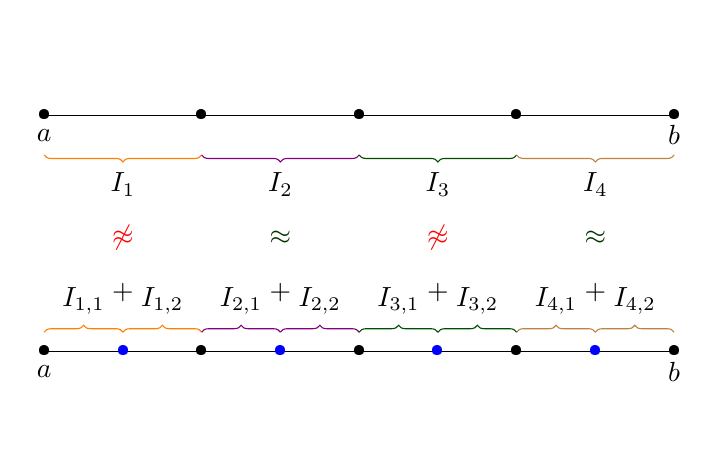
\begin{tikzpicture}
\node at (1,1) {};
\node at (1,-4) {};
% TRAIN
%\draw[<->, dashed] (0,0.5) -- (2,0.5);
%\node at (1,0.75) {$h$};
\draw (0,0) -- (8,0);
\foreach \Point in {(0,0), (2,0), (4,0), (6,0), (8,0)}{\node at \Point {\textbullet};}
\node at (0,-0.25) {$a$};
\node at (8,-0.25) {$b$};

\draw [orange, decorate, decoration = {brace,mirror}] (0,-0.5) -- (2,-0.5)node[pos=0.5,below=3pt,black]{$I_{1}$};

\draw [violet, decorate, decoration = {brace,mirror}] (2,-0.5) -- (4,-0.5)node[pos=0.5,below=3pt,black]{$I_{2}$};

\draw [green!30!black, decorate, decoration = {brace,mirror}] (4,-0.5) -- (6,-0.5)node[pos=0.5,below=3pt,black]{$I_{3}$};

\draw [brown, decorate, decoration = {brace,mirror}] (6,-0.5) -- (8,-0.5)node[pos=0.5,below=3pt,black]{$I_{4}$};

% VALIDATION
%\draw[<->, dashed] (0,-3.5) -- (1,-3.5);
%\node at (0.5,-3.75) {$h/2$};

\draw (0,-3) -- (8,-3);
\foreach \Point in {(0,-3), (2,-3), (4,-3), (6,-3), (8,-3)}{\node at \Point {\textbullet};}
\foreach \Point in {(1,-3), (3,-3), (5,-3), (7,-3)}{\node[blue] at \Point {\textbullet};}
\node at (0,-3.25) {$a$};
\node at (8,-3.25) {$b$};

\draw [orange, decorate, decoration = {brace}] (0,-2.75) -- (1,-2.75)node[pos=0.5,above=3pt,black]{$I_{1,1}$};
\draw [orange, decorate, decoration = {brace}] (1,-2.75) -- (2,-2.75)node[pos=0.5,above=3pt,black]{$I_{1,2}$};
\node at (1, -2.25) {$+$};
\node at (1, -1.55) {\textcolor{red}{$\not\approx$}};

\draw [violet, decorate, decoration = {brace}] (2,-2.75) -- (3,-2.75)node[pos=0.5,above=3pt,black]{$I_{2,1}$};
\draw [violet, decorate, decoration = {brace}] (3,-2.75) -- (4,-2.75)node[pos=0.5,above=3pt,black]{$I_{2,2}$};
\node at (3, -2.25) {$+$};
\node at (3, -1.55) {\textcolor{green!20!black}{$\approx$}};

\draw [green!30!black, decorate, decoration = {brace}] (4,-2.75) -- (5,-2.75)node[pos=0.5,above=3pt,black]{$I_{3,1}$};
\draw [green!30!black, decorate, decoration = {brace}] (5,-2.75) -- (6,-2.75)node[pos=0.5,above=3pt,black]{$I_{3,2}$};
\node at (5, -2.25) {$+$};
\node at (5, -1.55) {\textcolor{red}{$\not\approx$}};

\draw [brown, decorate, decoration = {brace}] (6,-2.75) -- (7,-2.75)node[pos=0.5,above=3pt,black]{$I_{4,1}$};
\draw [brown, decorate, decoration = {brace}] (7,-2.75) -- (8,-2.75)node[pos=0.5,above=3pt,black]{$I_{4,2}$};
\node at (7, -2.25) {$+$};
\node at (7, -1.55) {\textcolor{green!20!black}{$\approx$}};
\end{tikzpicture}
		\label{fig:adaptive_1}
 	\end{figure}
\end{column}

\begin{column}{0.3\textwidth}
Training set

\vspace{2.5cm}

Validation set
\end{column}
\end{columns}
 } 

\only<4-4>{
\centering
\begin{columns}
\begin{column}{0.7\textwidth}
	\begin{figure}[!htp]
		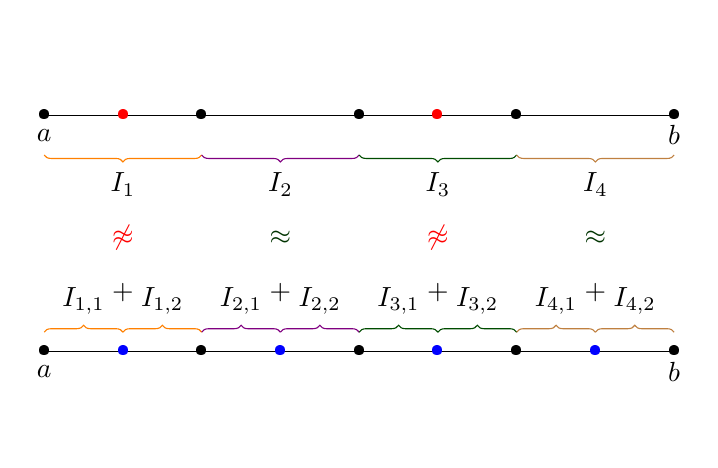
\begin{tikzpicture}
\node at (1,1) {};
\node at (1,-4) {};
% TRAIN
%\draw[<->, dashed] (0,0.5) -- (2,0.5);
%\node at (1,0.75) {$h$};
\draw (0,0) -- (8,0);
\foreach \Point in {(0,0), (2,0), (4,0), (6,0), (8,0)}{\node at \Point {\textbullet};}
\node at (0,-0.25) {$a$};
\node at (8,-0.25) {$b$};

\foreach \Point in {(1,0), (5,0)}{\node[red] at \Point {\textbullet};}

\draw [orange, decorate, decoration = {brace,mirror}] (0,-0.5) -- (2,-0.5)node[pos=0.5,below=3pt,black]{$I_{1}$};

\draw [violet, decorate, decoration = {brace,mirror}] (2,-0.5) -- (4,-0.5)node[pos=0.5,below=3pt,black]{$I_{2}$};

\draw [green!30!black, decorate, decoration = {brace,mirror}] (4,-0.5) -- (6,-0.5)node[pos=0.5,below=3pt,black]{$I_{3}$};

\draw [brown, decorate, decoration = {brace,mirror}] (6,-0.5) -- (8,-0.5)node[pos=0.5,below=3pt,black]{$I_{4}$};

% VALIDATION
%\draw[<->, dashed] (0,-3.5) -- (1,-3.5);
%\node at (0.5,-3.75) {$h/2$};

\draw (0,-3) -- (8,-3);
\foreach \Point in {(0,-3), (2,-3), (4,-3), (6,-3), (8,-3)}{\node at \Point {\textbullet};}
\foreach \Point in {(1,-3), (3,-3), (5,-3), (7,-3)}{\node[blue] at \Point {\textbullet};}
\node at (0,-3.25) {$a$};
\node at (8,-3.25) {$b$};

%\foreach \Point in {(0.5,-3), (1.5,-3), (4.5,-3), (5.5,-3)}{\node[red] at \Point {\textbullet};}

\draw [orange, decorate, decoration = {brace}] (0,-2.75) -- (1,-2.75)node[pos=0.5,above=3pt,black]{$I_{1,1}$};
\draw [orange, decorate, decoration = {brace}] (1,-2.75) -- (2,-2.75)node[pos=0.5,above=3pt,black]{$I_{1,2}$};
\node at (1, -2.25) {$+$};
\node at (1, -1.55) {\textcolor{red}{$\not\approx$}};

\draw [violet, decorate, decoration = {brace}] (2,-2.75) -- (3,-2.75)node[pos=0.5,above=3pt,black]{$I_{2,1}$};
\draw [violet, decorate, decoration = {brace}] (3,-2.75) -- (4,-2.75)node[pos=0.5,above=3pt,black]{$I_{2,2}$};
\node at (3, -2.25) {$+$};
\node at (3, -1.55) {\textcolor{green!20!black}{$\approx$}};

\draw [green!30!black, decorate, decoration = {brace}] (4,-2.75) -- (5,-2.75)node[pos=0.5,above=3pt,black]{$I_{3,1}$};
\draw [green!30!black, decorate, decoration = {brace}] (5,-2.75) -- (6,-2.75)node[pos=0.5,above=3pt,black]{$I_{3,2}$};
\node at (5, -2.25) {$+$};
\node at (5, -1.55) {\textcolor{red}{$\not\approx$}};

\draw [brown, decorate, decoration = {brace}] (6,-2.75) -- (7,-2.75)node[pos=0.5,above=3pt,black]{$I_{4,1}$};
\draw [brown, decorate, decoration = {brace}] (7,-2.75) -- (8,-2.75)node[pos=0.5,above=3pt,black]{$I_{4,2}$};
\node at (7, -2.25) {$+$};
\node at (7, -1.55) {\textcolor{green!20!black}{$\approx$}};
\end{tikzpicture}
		\label{fig:adaptive_1}
 	\end{figure}
\end{column}

\begin{column}{0.3\textwidth}
Training set 

\vspace{2.5cm}

Validation set
\end{column}
\end{columns}
 }

\only<5-5>{
\centering
\begin{columns}
\begin{column}{0.7\textwidth}
	\begin{figure}[!htp]
		\begin{tikzpicture}
\node at (1,1) {};
\node at (1,-4) {};
% TRAIN
%\draw[<->, dashed] (0,0.5) -- (2,0.5);
%\node at (1,0.75) {$h$};
\draw (0,0) -- (8,0);
\foreach \Point in {(0,0), (2,0), (4,0), (6,0), (8,0)}{\node at \Point {\textbullet};}
\node at (0,-0.25) {$a$};
\node at (8,-0.25) {$b$};

\foreach \Point in {(1,0), (5,0)}{\node at \Point {\textbullet};}

%\draw [orange, decorate, decoration = {brace,mirror}] (0,-0.5) -- (2,-0.5)node[pos=0.5,below=3pt,black]{$I_{1}$};
%
%\draw [violet, decorate, decoration = {brace,mirror}] (2,-0.5) -- (4,-0.5)node[pos=0.5,below=3pt,black]{$I_{2}$};
%
%\draw [green!30!black, decorate, decoration = {brace,mirror}] (4,-0.5) -- (6,-0.5)node[pos=0.5,below=3pt,black]{$I_{3}$};
%
%\draw [brown, decorate, decoration = {brace,mirror}] (6,-0.5) -- (8,-0.5)node[pos=0.5,below=3pt,black]{$I_{4}$};

% VALIDATION
%\draw[<->, dashed] (0,-3.5) -- (1,-3.5);
%\node at (0.5,-3.75) {$h/2$};

\draw (0,-3) -- (8,-3);
\foreach \Point in {(0,-3),(1,-3), (2,-3), (4,-3),(5,-3), (6,-3), (8,-3)}{\node at \Point {\textbullet};}
\foreach \Point in { (0.5,-3), (1.5,-3),(3,-3), (4.5,-3), (5.5,-3), (7,-3)}{\node[blue] at \Point {\textbullet};}
\node at (0,-3.25) {$a$};
\node at (8,-3.25) {$b$};

%\draw [orange, decorate, decoration = {brace}] (0,-2.75) -- (1,-2.75)node[pos=0.5,above=3pt,black]{$I_{1,1}$};
%\draw [orange, decorate, decoration = {brace}] (1,-2.75) -- (2,-2.75)node[pos=0.5,above=3pt,black]{$I_{1,2}$};
%\node at (1, -2.25) {$+$};
%\node at (1, -1.55) {\textcolor{red}{$\not\approx$}};
%
%\draw [violet, decorate, decoration = {brace}] (2,-2.75) -- (3,-2.75)node[pos=0.5,above=3pt,black]{$I_{2,1}$};
%\draw [violet, decorate, decoration = {brace}] (3,-2.75) -- (4,-2.75)node[pos=0.5,above=3pt,black]{$I_{2,2}$};
%\node at (3, -2.25) {$+$};
%\node at (3, -1.55) {\textcolor{green!20!black}{$\approx$}};
%
%\draw [green!30!black, decorate, decoration = {brace}] (4,-2.75) -- (5,-2.75)node[pos=0.5,above=3pt,black]{$I_{3,1}$};
%\draw [green!30!black, decorate, decoration = {brace}] (5,-2.75) -- (6,-2.75)node[pos=0.5,above=3pt,black]{$I_{3,2}$};
%\node at (5, -2.25) {$+$};
%\node at (5, -1.55) {\textcolor{red}{$\not\approx$}};
%
%\draw [brown, decorate, decoration = {brace}] (6,-2.75) -- (7,-2.75)node[pos=0.5,above=3pt,black]{$I_{4,1}$};
%\draw [brown, decorate, decoration = {brace}] (7,-2.75) -- (8,-2.75)node[pos=0.5,above=3pt,black]{$I_{4,2}$};
%\node at (7, -2.25) {$+$};
%\node at (7, -1.55) {\textcolor{green!20!black}{$\approx$}};
\end{tikzpicture}
		\label{fig:adaptive_1}
 	\end{figure}
\end{column}

\begin{column}{0.3\textwidth}
Training set 

\vspace{2.5cm}

Validation set
\end{column}
\end{columns}
 } 
\end{frame}


\begin{frame}{Adaptive Integration}
\vspace{0.25cm}
\begin{itemize}
\item[\tickNo] Mesh based
\vspace{0.15cm}

\item[\tickYes] Appropiate for low dimensional problems
\vspace{0.15cm}

\item[\tickYes] Allows the use of autodiff to compute $\nabla u$
\vspace{0.15cm}
\end{itemize}
\end{frame}


\begin{frame}{Piecewise-polynomial approximation}

%\begin{itemize}
%\item We define a mesh
%\end{itemize}
%
%\begin{center}
%\begin{tikzpicture}
%\draw (0,0) -- (8,0);
%\draw[red,fill=red] (0,0) circle (0.7ex);
%\draw[violet,fill=violet] (8,0) circle (0.7ex);
%\node [red] at (0,-0.4){$\Gamma_D$};
%\node [violet] at (8,-0.4){$\Gamma_N$};
%%
%\foreach \Point in {(2,0), (4,0), (6,0)}{\draw[fill=black] \Point circle (0.5ex);}
%\end{tikzpicture}
%\end{center}

\begin{itemize}
\item We define a mesh $\mathcal{T}$ composed by a  set of nodes $\{ x_{node} \}_{i=1}^{k}$
\item We select the degree $p$ of the polynomial.
\item We build the approximate piecewise solution $u^{*}_{NN,k-1} (x_{node}, u_{NN}(x_{node}))$ .
\end{itemize}

\vspace{0.5cm}
\begin{columns}
%
\begin{column}{0.45\textwidth}
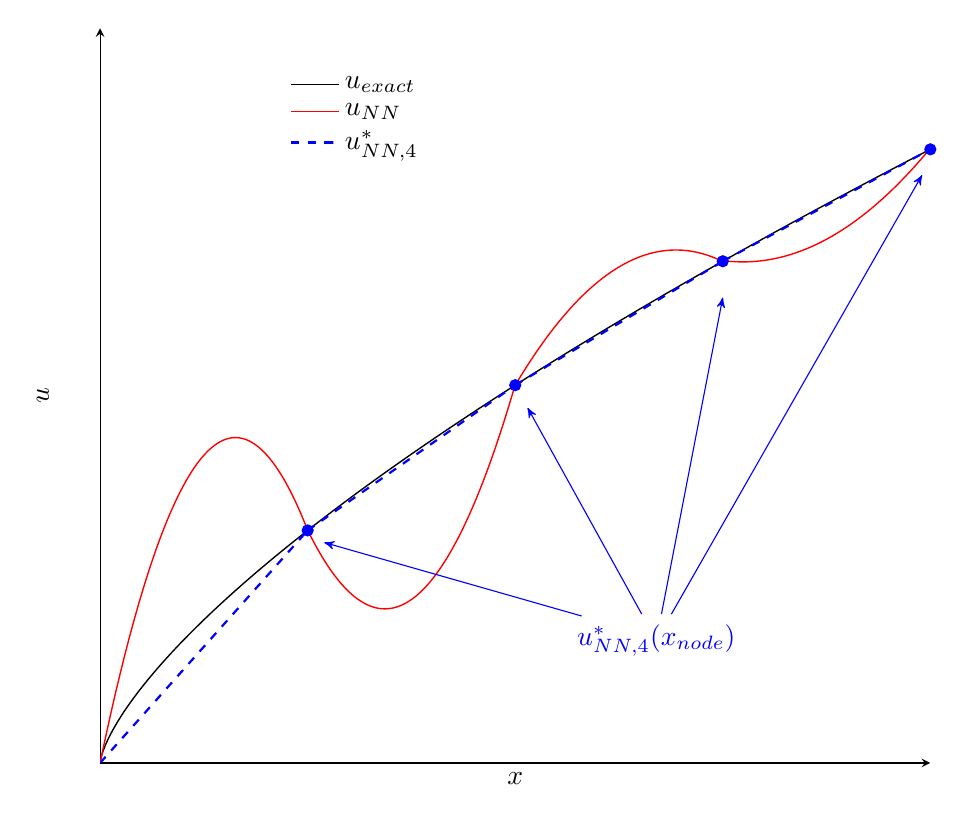
\begin{tikzpicture}
    \begin{axis}[
    xlabel = {$x$},
    xmin=0,
    xmax=10,
    ymin=0,
    ymax=6,
    ylabel = {$u$},
      height=0.9*\textwidth,
      width=1*\textwidth,
    axis lines=left,
    ticks=none,
%    grid=both,
	%xtick={0,0.25,...,1},
	%ytick={0,100},
    %yticklabels={0,$a$},
    y label style={at={(-0.05,0.5)}},
%    xticklabels={-3,-1,...,5},
%    ticks=xticklabels,
    legend columns = 1,
    legend style= {at={(0.4,0.95)},draw=none,fill=none,nodes={scale=1, transform shape}}, legend cell align={left}]
    ]    
    \tikzset{ dot/.style = {circle, fill, minimum size=3pt, inner sep=0pt, outer sep=0pt}, }
% exact 
\addplot[samples=500,color=black, smooth, line width=0.5, domain=0:10] {x^0.7};	
\addlegendentry{$u_{exact}$};

%% u_NN
\addplot[samples=500,color=red, smooth, line width=0.5, domain=0:2.5] {-x^2+3.26*x };
\addlegendentry{$u_{NN}$}
\addplot[samples=10,color=blue, smooth, dashed, domain=0:2.5, line width=0.8] {1.899/2.5*x};
\addlegendentry{$u^{*}_{NN,4}$ }
%
%
%%%%%%%% WE NEED TO PUT THE FIRST THREE PLOTS DIFFERENT TO OBTAIN THE CORRECT LEGEND IN THE PLOT
%
%%% u_NN
\addplot[samples=500,color=red, smooth, line width=0.5, domain=2.5:5] {0.743*(x^2)-5.097*x +10};
\addplot[samples=500,color=red, smooth, line width=0.5, domain=5:7.5] {-0.295*(x^2)+4.0918*x -10};
\addplot[samples=500,color=red, smooth, line width=0.5, domain=7.5:10] {0.182*(x^2)-2.818*x +15};

%% u_p
\draw[color=blue, smooth, dashed, line width=0.8] (2.5,1.899) -- (5,3.085);
\draw[color=blue, smooth, dashed, line width=0.8] (5,3.085) -- (7.5,4.097);
\draw[color=blue, smooth, dashed, line width=0.8] (7.5,4.097) -- (10,5.011);

%%points
\addplot[only marks,mark=*,blue,mark size=2pt] coordinates {(2.5,1.899)(5,3.085)(7.5,4.097)(10,5.011)};

    \tikzstyle{state}=[
        draw = white,
        thick,
        fill = white,
        minimum width=15mm, 
        minimum height=4mm
    ]

\node(G)[ state,  ] at (axis cs: 6.7,1.) {\textcolor{blue}{$u^{*}_{NN,4}(x_{node})$}};
%\node(G_aux1)[anchor = north, text width=1.0] at (axis cs: 1.65,31) {};
%\node(G_aux2)[anchor = north, text width=1.0] at (axis cs: 2,31) {};
    

%\node (G1) at (axis cs: 0.28175, 19){};
%\node (G2) at (axis cs: 1.25, 46.27){};
%\node (G3) at (axis cs: 2.21825, 36.05){};
%
%\draw[] (G1) node[above, blue] {};
%\draw[] (G2) node[above, blue] {};
%\draw[] (G3) node[above, blue] {};


\path[->, blue] (axis cs: 5.8,1.2) edge (axis cs:2.7,1.8);
\path[->, blue] (G) edge (axis cs:5.15,2.9);
\path[->, blue] (G) edge (axis cs:7.5,3.8);
\path[->, blue] (G) edge (axis cs:9.9,4.8);

\end{axis}
\end{tikzpicture}
\end{column}
%
\begin{column}{0.55\textwidth}
\begin{itemize}
\item[\tickNo]  Mesh based method
\item[\tickYes] Appropriate for low dimensions
\item[\tickYes] Allows exact integration $\&$ differentiation
\item[\tickNo]  It does not allow the use of autodiff
\item[\tickYes] Exists theory about its convergence
\end{itemize}
\end{column}
\end{columns}
\end{frame}
%%%%%%%%%%%%%%%%%%%%%%%%%%%%%%%%%%%%%%%%%%%%%%%%%%%%%%%%%%%%%%%%%%%%


\begin{frame}[t]{Numerical Results}
\only<1-1>{
\textbf{Piecewise-linear approximation:}

Mesh with four and ten elements. One Gauss point per element. $u_{exact}=x^{0.7}$.
%\vspace{0.5cm}

\begin{minipage}{.45\textwidth}
\begin{figure}[!htp]
\centering
\begin{tikzpicture}
%https://tex.stackexchange.com/questions/451704/tikz-position-of-an-imported-image
  \node[anchor=south west,inner sep=0] (image) at (0,0) {\begin{tikzpicture}
\begin{axis}[scale only axis, xlabel = $x$, ylabel = $u$, ytick pos=left, y label style={at={(-0.1,0.5)}}, legend style= {at={(0.3,0.95)}, fill=none,draw=none,nodes={scale=1.0, transform shape}}, legend cell align={left}, height=4cm, width=4cm, xmin=-0.2, ymin=0, xmax=10.2, ymax=5.5,samples=1000, xticklabel style={yshift=-3pt}, yticklabel style={xshift=-3pt}]
%\addlegendimage{only marks, mark size=4pt, mark=-, color=black} 
%\addlegendimage{only marks, mark size=4pt, mark=-, color=red}
\addplot [black, line width=1pt,domain=0:10] {x^0.7};
%\addlegendentry{\textcolor{black}{$u_{exact}$}}
\addplot[line width=0.7pt,color=red] %
	table[x=x ,y=u_pred]{Diapos/PDEs_with_NN/Figures/Alternatives//Data//data_Ritz_FD_4elem.csv};
%\addlegendentry{\textcolor{red}{$u_{NN}$ 4 elem}}
\addplot[line width=0.7pt,color=blue] %
	table[x=x ,y=u_pred]{Diapos/PDEs_with_NN/Figures/Alternatives//Data//data_Ritz_FD_10elem.csv};
%\addlegendentry{\textcolor{blue}{$u_{NN}$ 10 elem}}
% Legend
%\node[anchor = south] (Ua)at (3,4.5){\textcolor{red}{$u_{\varphi}$}};
%\node[anchor = south] at (3,4){\textcolor{black}{$u_{exact}$}};
\end{axis}
\end{tikzpicture}
};
  \begin{scope}[x={(image.south east)},y={(image.north west)}]
  \draw[<-, color=red] (0.3,0.35) -- (0.5,0.3) node[right, text width=0.925cm] {\textcolor{red}{$u^{*}_{NN,4}$}};
    \draw[<-, color=blue] (0.58,0.7) -- (0.5,0.8) node[above left, text width=1.09cm] {\textcolor{blue}{$u^{*}_{NN,10}$}};
  \draw[<-] (0.37,0.53) -- (0.3,0.6) node[above] {$u_{exact}$};
  \end{scope}
\end{tikzpicture}

 \end{figure}
\end{minipage}%
\hspace{1.5cm}
\begin{minipage}{.35\textwidth}
\vspace{0.9cm}
\begin{figure}[!htp]
\centering
\begin{tikzpicture}
%https://tex.stackexchange.com/questions/451704/tikz-position-of-an-imported-image
  \node[anchor=south west,inner sep=0] (image) at (0,0) {\begin{tikzpicture}
\begin{axis}[scale only axis, xlabel = $Epoch$, ylabel = $Loss$, ytick pos=left, y label style={at={(-0.15,0.5)}}, x label style={at={(0.5,-0.15)}}, legend style= {at={(0.97,0.95)},draw=none,fill=none,nodes={scale=0.8, transform shape}}, legend cell align={left}, height=4cm, width=4cm, xmin=0.95, ymin=-2, xmax=40000, ymax=4, ytick = {2,0,-1.54}, xmode=log, xticklabel style={yshift=-3pt}, yticklabel style={xshift=-3pt}]
\addplot [black, dashed, line width=0.7pt,domain=0.99999:39900] {-1.54};
%\addlegendentry{Loss of exact solution}
\addplot[line width=0.8pt,color=red] %
	table[x=epoch ,y=loss]{Diapos/PDEs_with_NN/Figures/Alternatives//Data//loss_Ritz_FD_4elem_treshold.csv};
%\addlegendentry{Loss of NN approximation 4 elem.};
\addplot[line width=0.8pt,color=blue] %
	table[x=epoch ,y=loss]{Diapos/PDEs_with_NN/Figures/Alternatives//Data//loss_Ritz_FD_10elem_treshold.csv};
%\addlegendentry{Loss of NN approximation 10 elem.};

% Legend
%\node[anchor = south] (Ua)at (6,32){\textcolor{red}{$u_{approx}$}};
%\node[anchor = south] at (6,6){\textcolor{black}{$u_{exact}$}};

\end{axis}
\end{tikzpicture}
};
  \begin{scope}[x={(image.south east)},y={(image.north west)}]
%  \draw[<-, color=red] (0.355,0.26) -- (0.355,0.29) node[above] {\textcolor{red}{{\small $\mathcal{F}_{R}(u_{exact})$}}};
  \node[] at (0.37,0.3) (c) {\textcolor{black}{{\small $\mathcal{L}_{\mathcal{R}}(u_{exact})$}}};
  \draw[<-,red] (0.53,0.36) -- (0.6,0.75) node[above, text width=1.3cm] {\textcolor{red}{{\small $\mathcal{L}_{\mathcal{R}}(u^{*}_{NN,4})$}}};
  \draw[<-, color=blue] (0.61,0.36) -- (0.8,0.45) node[above, text width=1.5cm] {\textcolor{blue}{{\small $\mathcal{L}_{\mathcal{R}}(u^{*}_{NN,10})$}}};
  \end{scope}
\end{tikzpicture}

 \end{figure}
\end{minipage}%
}

 \only<2-2>{
\textbf{Adaptive integration:}

Mesh with four elements. Three Gauss points per element. $u_{exact}=x^{0.7}$.
%\vspace{0.5cm}

\begin{minipage}{.45\textwidth}
\begin{figure}[!htp]
\centering
\begin{tikzpicture}
%https://tex.stackexchange.com/questions/451704/tikz-position-of-an-imported-image
  \node[anchor=south west,inner sep=0] (image) at (0,0) {\begin{tikzpicture}
\begin{axis}[scale only axis, xlabel = $x$, ylabel = $u$, ytick pos=left, y label style={at={(-0.1,0.5)}}, legend style= {at={(0.3,0.95)}, fill=none,draw=none,nodes={scale=1.0, transform shape}}, legend cell align={left}, height=4cm, width=4cm, xmin=-0.2, ymin=0, xmax=10.2, ymax=5.5,samples=1000, xticklabel style={yshift=-3pt}, yticklabel style={xshift=-3pt}]
\addlegendimage{only marks, mark size=4pt, mark=-, color=black} 
\addlegendimage{only marks, mark size=4pt, mark=-, color=red}
\addplot [black, line width=2pt,domain=0:10] {x^0.7};
%\addlegendentry{\textcolor{black}{$u_{exact}$}}
\addplot[line width=0.7pt,color=red] %
	table[x=x ,y=u_pred]{Diapos/PDEs_with_NN/Figures/Alternatives//Data//data_Ritz_adaptive.csv};
%\addlegendentry{\textcolor{red}{$u_{NN}$}}
\end{axis}
\end{tikzpicture}
};
  \begin{scope}[x={(image.south east)},y={(image.north west)}]
  \draw[<-, color=red] (0.4,0.35) -- (0.55,0.3) node[below right] {\textcolor{red}{$u_{NN}$}};
  \draw[<-] (0.62,0.7) -- (0.45,0.8) node[above left] {$u_{exact}$};
  \end{scope}
\end{tikzpicture}

 \end{figure}
\end{minipage}%
\hspace{1.5cm}
\begin{minipage}{.35\textwidth}
\vspace{0.9cm}
\begin{figure}[!htp]
\centering
\begin{tikzpicture}
%https://tex.stackexchange.com/questions/451704/tikz-position-of-an-imported-image
  \node[anchor=south west,inner sep=0] (image) at (0,0) {\begin{tikzpicture}
\begin{axis}[scale only axis, xlabel = $Epoch$, ylabel = $Loss$, ytick pos=left, y label style={at={(-0.1,0.5)}}, x label style={at={(0.5,-0.15)}}, legend style= {at={(0.95,0.95)},draw=none,fill=none,nodes={scale=0.8, transform shape}}, legend cell align={left}, height=4cm, width=4cm, xmin=0.95, ymin=-2, xmax=40000, ymax=10, ytick = {8,-1.54}, xmode=log, xticklabel style={yshift=-3pt}, yticklabel style={xshift=-3pt}]
\addplot [black, dashed, line width=0.7pt,domain=0.99999:39900] {-1.54};
%\addlegendentry{Loss of exact solution}
\addplot[line width=0.8pt,color=red] %
	table[x=epoch ,y=loss]{Diapos/PDEs_with_NN/Figures/Alternatives//Data//loss_Ritz_adaptivity_treshold.csv};
%\addlegendentry{Loss of NN approximation.};

% Legend
%\node[anchor = south] (Ua)at (6,32){\textcolor{red}{$u_{approx}$}};
%\node[anchor = south] at (6,6){\textcolor{black}{$u_{exact}$}};

\end{axis}
\end{tikzpicture}
};
  \begin{scope}[x={(image.south east)},y={(image.north west)}]
  \draw[<-, color=black] (0.33,0.23) -- (0.6,0.45) node[above right] {\textcolor{black}{$\mathcal{L}_{\mathcal{R}}(u_{exact})$}};
  \draw[<-, color=red] (0.32,0.67) -- (0.6,0.85) node[above right] {\textcolor{red}{$\mathcal{L}_{\mathcal{R}}(u_{NN})$}};
  \end{scope}
\end{tikzpicture}

 \end{figure}
\end{minipage}%
 }
 
 \only<3-3>{
 \textbf{Regularization:}
 Minimization of the energy $\int_0^{10} \frac{1}{2}u'(x)^2+2u(x)\,dx+u(10)$ with $u(0)=0$ and mid-point rule. $u_{exact}=x^{2}$.
 \vspace{0.5cm}
% \begin{figure}[!htp]
% \centering
%    \begin{tikzpicture}
%https://tex.stackexchange.com/questions/451704/tikz-position-of-an-imported-image
\node at (0,0) {};
  \node[anchor=south west,inner sep=0] (image) at (0.05,0.03) {\begin{tikzpicture}
\begin{axis}[scale only axis, xlabel = $x$, ylabel = $u$, ytick pos=left, y label style={at={(-0.15,0.5)}}, legend style= {at={(0.3,0.95)}, fill=none,draw=none,nodes={scale=1.0, transform shape}}, legend cell align={left}, height=4cm, width=4cm, xmin=-0.2, ymin=-40, xmax=10.2, ymax=110,samples=10000, xticklabel style={yshift=-3pt}, yticklabel style={xshift=-3pt}]
\addlegendimage{only marks, mark size=4pt, mark=-, color=black} 
\addlegendimage{only marks, mark size=4pt, mark=-, color=red}
\addplot [black, line width=1pt,domain=0:10] {x^2};
%\addlegendentry{\textcolor{black}{$u_{exact}$}}
\addplot[line width=0.7pt,color=red] %
	table[x=x ,y=u_pred]{Diapos/PDEs_with_NN/Figures/Alternatives//Data//data_NoRegN50M10_sol.txt};
%\addlegendentry{\textcolor{red}{$u_{NN}$}}
\end{axis}
\end{tikzpicture}
};
  \begin{scope}[x={(image.south east)},y={(image.north west)}]
  \draw[<-, color=red] (0.27,0.3) -- (0.35,0.25) node[right] {\textcolor{red}{$u_{NN}$}};
  \draw[<-] (0.55,0.45) -- (0.65,0.4) node[below right] {$u_{exact}$};
  \end{scope}
\end{tikzpicture}

%    	\hspace{1cm}
%	\begin{tikzpicture}
%https://tex.stackexchange.com/questions/451704/tikz-position-of-an-imported-image
  \node[anchor=south west,inner sep=0] (image) at (0,0) {\begin{tikzpicture}
\begin{axis}[scale only axis, xlabel = $Epoch$, ylabel = $Loss$, ytick pos=left, y label style={at={(-0.1,0.5)}}, x label style={at={(0.5,-0.15)}}, legend style= {at={(0.95,0.95)},draw=none,fill=none,nodes={scale=0.8, transform shape}}, legend cell align={left}, height=4cm, width=4cm, xmin=0.95, xmax=30000, xmode=log, xticklabel style={yshift=-3pt}, yticklabel style={xshift=-3pt}]
%\addplot [red, dashed, line width=0.7pt,domain=0.99999:200000] {-666.67};
%\addlegendentry{Loss of exact solution}
\addplot[line width=0.8pt,color=black] %
	table[x=iter ,y=loss]{Diapos/PDEs_with_NN/Figures/Alternatives//Data//data_NoRegN50M10_R.txt};
%\addlegendentry{Loss $\mathcal{R}$};
\end{axis}
\end{tikzpicture}
};
  \begin{scope}[x={(image.south east)},y={(image.north west)}]
  \draw[<-] (0.95,0.7) -- (0.75,0.75) node[above left] {Loss $R$};
  \end{scope}
\end{tikzpicture}

%  \end{figure}
  
  \begin{minipage}{.45\textwidth}
\begin{figure}[!htp]
\centering
\begin{tikzpicture}
%https://tex.stackexchange.com/questions/451704/tikz-position-of-an-imported-image
\node at (0,0) {};
  \node[anchor=south west,inner sep=0] (image) at (0.05,0.03) {\begin{tikzpicture}
\begin{axis}[scale only axis, xlabel = $x$, ylabel = $u$, ytick pos=left, y label style={at={(-0.15,0.5)}}, legend style= {at={(0.3,0.95)}, fill=none,draw=none,nodes={scale=1.0, transform shape}}, legend cell align={left}, height=4cm, width=4cm, xmin=-0.2, ymin=-40, xmax=10.2, ymax=110,samples=10000, xticklabel style={yshift=-3pt}, yticklabel style={xshift=-3pt}]
\addlegendimage{only marks, mark size=4pt, mark=-, color=black} 
\addlegendimage{only marks, mark size=4pt, mark=-, color=red}
\addplot [black, line width=1pt,domain=0:10] {x^2};
%\addlegendentry{\textcolor{black}{$u_{exact}$}}
\addplot[line width=0.7pt,color=red] %
	table[x=x ,y=u_pred]{Diapos/PDEs_with_NN/Figures/Alternatives//Data//data_NoRegN50M10_sol.txt};
%\addlegendentry{\textcolor{red}{$u_{NN}$}}
\end{axis}
\end{tikzpicture}
};
  \begin{scope}[x={(image.south east)},y={(image.north west)}]
  \draw[<-, color=red] (0.27,0.3) -- (0.35,0.25) node[right] {\textcolor{red}{$u_{NN}$}};
  \draw[<-] (0.55,0.45) -- (0.65,0.4) node[below right] {$u_{exact}$};
  \end{scope}
\end{tikzpicture}

 \end{figure}
\end{minipage}%
\hspace{1.5cm}
\begin{minipage}{.35\textwidth}
\vspace{-0.25cm}
\begin{figure}[!htp]
\centering
\begin{tikzpicture}
%https://tex.stackexchange.com/questions/451704/tikz-position-of-an-imported-image
  \node[anchor=south west,inner sep=0] (image) at (0,0) {\begin{tikzpicture}
\begin{axis}[scale only axis, xlabel = $Epoch$, ylabel = $Loss$, ytick pos=left, y label style={at={(-0.1,0.5)}}, x label style={at={(0.5,-0.15)}}, legend style= {at={(0.95,0.95)},draw=none,fill=none,nodes={scale=0.8, transform shape}}, legend cell align={left}, height=4cm, width=4cm, xmin=0.95, xmax=30000, xmode=log, xticklabel style={yshift=-3pt}, yticklabel style={xshift=-3pt}]
%\addplot [red, dashed, line width=0.7pt,domain=0.99999:200000] {-666.67};
%\addlegendentry{Loss of exact solution}
\addplot[line width=0.8pt,color=black] %
	table[x=iter ,y=loss]{Diapos/PDEs_with_NN/Figures/Alternatives//Data//data_NoRegN50M10_R.txt};
%\addlegendentry{Loss $\mathcal{R}$};
\end{axis}
\end{tikzpicture}
};
  \begin{scope}[x={(image.south east)},y={(image.north west)}]
  \draw[<-] (0.95,0.7) -- (0.75,0.75) node[above left] {Loss $R$};
  \end{scope}
\end{tikzpicture}

 \end{figure}
\end{minipage}%
 }
 
\only<4-4>{
 \textbf{Regularization:}
 Minimization of the energy $\int_0^{10} \frac{1}{2}u'(x)^2+2u(x)\,dx+u(10)$ with $u(0)=0$ and mid-point rule. $u_{exact}=x^{2}$.
 \vspace{0.35cm}
 
\begin{minipage}{.45\textwidth}
\begin{figure}[!htp]
\centering
\begin{tikzpicture}
%https://tex.stackexchange.com/questions/451704/tikz-position-of-an-imported-image
\node at (0,0) {};
  \node[anchor=south west,inner sep=0] (image) at (0.02,0.03) {\begin{tikzpicture}
\begin{axis}[scale only axis, xlabel = $x$, ylabel = $u$, ytick pos=left, y label style={at={(-0.2,0.5)}}, legend style= {at={(0.3,0.95)}, fill=none,draw=none,nodes={scale=1.0, transform shape}}, legend cell align={left}, height=4cm, width=4cm, xmin=-0.2, ymin=-0.5, xmax=10.2, ymax=110,samples=10000, xticklabel style={yshift=-3pt}, yticklabel style={xshift=-3pt}]
\addlegendimage{only marks, mark size=4pt, mark=-, color=black} 
\addlegendimage{only marks, mark size=4pt, mark=-, color=red}
\addplot [black, line width=1pt,domain=0:10] {x^2};
%\addlegendentry{\textcolor{black}{$u_{exact}$}}
\addplot[line width=0.7pt,color=red] %
	table[x=x ,y=u_pred]{Diapos/PDEs_with_NN/Figures/Alternatives//Data//data_RegN50M10_sol.txt};
%\addlegendentry{\textcolor{red}{$u_{NN}$}}
% Legend
%\node[anchor = south] (Ua)at (3,4.5){\textcolor{red}{$u_{\varphi}$}};
%\node[anchor = south] at (3,4){\textcolor{black}{$u_{exact}$}};
\end{axis}
\end{tikzpicture}
};
  \begin{scope}[x={(image.south east)},y={(image.north west)}]
  \draw[<-, color=red] (0.6,0.3) -- (0.7,0.25) node[right] {\textcolor{red}{$u_{NN}$}};
  \draw[<-] (0.78,0.67) -- (0.65,0.85) node[above] {$u_{exact}$};
  \end{scope}
\end{tikzpicture}

 \end{figure}
\end{minipage}%
\hspace{1.5cm}
\begin{minipage}{.35\textwidth}
\vspace{0.3cm}
\begin{figure}[!htp]
\centering
\begin{tikzpicture}
%https://tex.stackexchange.com/questions/451704/tikz-position-of-an-imported-image
  \node[anchor=south west,inner sep=0] (image) at (0,0) {\begin{tikzpicture}
\begin{axis}[scale only axis, xlabel = $Epoch$, ylabel = $Loss$, ytick pos=left, y label style={at={(-0.15,0.5)}}, legend style= {at={(0.7,0.95)},draw=none,fill=none,nodes={scale=0.8, transform shape}}, legend cell align={left}, height=4cm, width=4cm, xmin=0.95, xmax=15000, xmode=log, xticklabel style={yshift=-3pt}, yticklabel style={xshift=-3pt}]
%\addplot [red, dashed, line width=0.7pt,domain=0.99999:200000] {-666.67};
%\addlegendentry{Loss of exact solution}
\addplot[line width=0.8pt,color=black] %
	table[x=iter ,y=loss]{Diapos/PDEs_with_NN/Figures/Alternatives//Data//data_RegN50M10_R.txt};
%\addlegendentry{Loss $\mathcal{R}$};

% Legend
%\node[anchor = south] (Ua)at (6,32){\textcolor{red}{$u_{approx}$}};
%\node[anchor = south] at (6,6){\textcolor{black}{$u_{exact}$}};

\end{axis}
\end{tikzpicture}
};
  \begin{scope}[x={(image.south east)},y={(image.north west)}]
  \draw[<-] (0.7,0.57) -- (0.55,0.85) node[above left] {Loss $R$};
  \end{scope}
\end{tikzpicture}

 \end{figure}
\end{minipage}%
 }
 \end{frame}


\begin{frame}{Deep Neural Networks for Solving PDEs}
\begin{itemize}
\item Quadrature errors appear when solving PDEs using DL methods.
\vspace{0.5cm}
\item Selecting an adequate quadrature rule is critical.
\vspace{0.5cm}
\item For high dimensions Monte Carlo is adequate.
\vspace{0.5cm}
\item We propose adaptive integration for low dimensions.
\end{itemize}
\end{frame}
%\end{section}
%%%%%%%%%%%%%%%%%%%%%%%%%%%%%%%%%%
%%%%%%%%%%%%%%%%%%%%%%%%%%%%%%%%%%
\begin{section}{Main Achievements}
{
\usebackgroundtemplate{\tikz\node[opacity=0.1,inner sep=0] {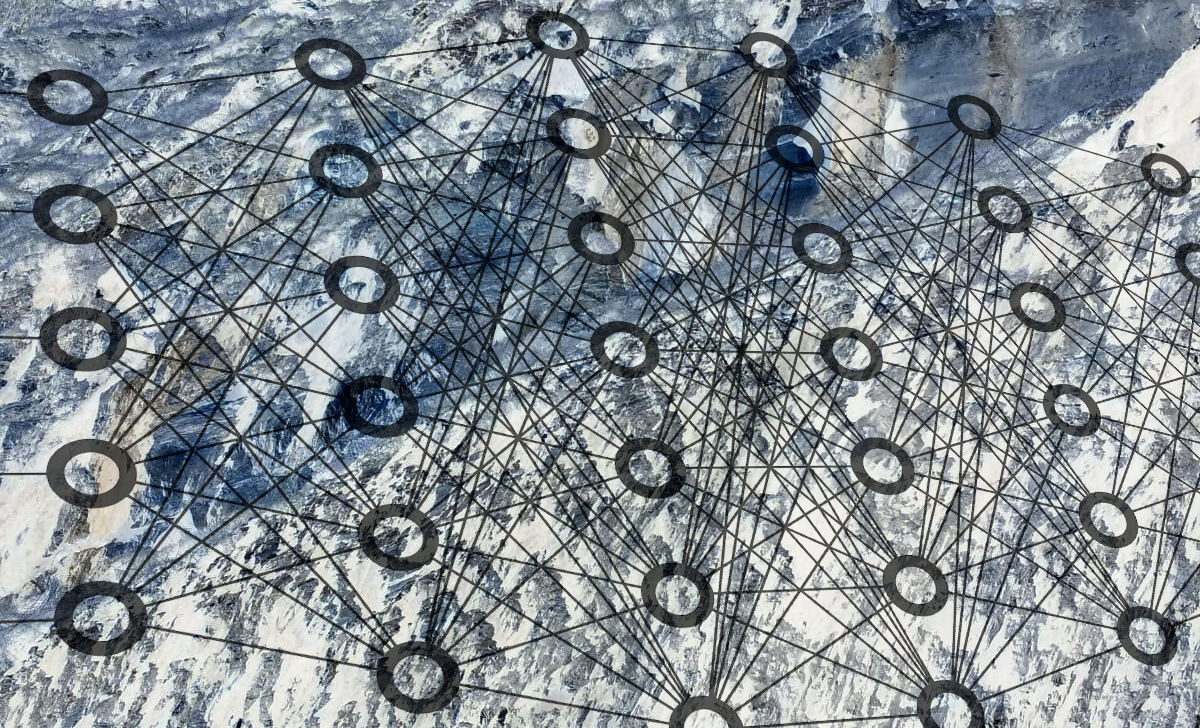
\includegraphics[height=\paperheight,width=\paperwidth]{frames/auxiliar/title_img/prueba.png}};}
%%%%%%%%
\begin{frame}[plain]

\begin{variableblock}{}{bg=myblue,fg=white}{bg=green,fg=red}
\begin{center}
\textbf{Main Achievements}
\end{center}
\end{variableblock}

\end{frame}
%%%%%%%%%%%%%%%%%%%%%%%%%%%%%%%%%%%%%%%%%%%%%%%%%%%%%%%%%%%%%%%%%%%
}
\begin{frame}{Main Achievements}
\textbf{Peer-Reviewed Publications}
\begin{thebibliography}{2}
\bibitem{mago}
{\small F. V. Caro, V. Darrigrand, J. Alvarez-Aramberri, and D. Pardo. ``A Multi-Adaptive-Goal-Oriented Strategy to Generate Massive Databases of Parametric PDEs,'' To be submitted to \textit{Computer Methods in Applied Mechanics and Engineering}, December 2023.}

\bibitem{painless}
{\small F. V. Caro, V. Darrigrand, J. Alvarez-Aramberri, E. Alberdi, and D. Pardo. ``A Painless Multi-Level Automatic Goal-Oriented $hp$-Adaptive Coarsening Strategy for Elliptic and Non-Elliptic Problems,'' \textit{Computer Methods in Applied Mechanics and Engineering}, vol. 401, 115641, 2022. \url{https://doi.org/10.1016/j.cma.2022.115641}}

\bibitem{ICCS}
{\small F. V. Caro, V. Darrigrand, J. Alvarez-Aramberri, E. A. Celaya, and D. Pardo. ``1D Painless Multi-Level Automatic Goal-Oriented $h$ and $p$ Adaptive Strategies Using a Pseudo-Dual Operator,'' In \textit{Computational Science -- ICCS 2022}, pp. 347--357, 2022. \url{https://doi.org/10.1007/978-3-031-08754-7_43}}
\end{thebibliography}
\end{frame}

\begin{frame}{Main Achievements}
\textbf{Conference Talks}
\vspace{0.2cm}

\begin{small}
\begin{tabular}{rl}
[1]& \underline{F. V. Caro}, V. Darrigrand, J. Alvarez-Aramberri, and D. Pardo. \\
& \textit{Databases for Deep Learning Inversion Using A Goal-Oriented $hp$-Adaptive Strategy.} \\
& XI International Conference on Adaptive Modeling and Simulation, \\
& Gothenburg, Sweden, June 19-21, 2023. \\\\
\end{tabular}

\begin{tabular}{rl}
[2]& \underline{F. V. Caro}, V. Darrigrand, J. Alvarez-Aramberri, E. Alberdi, and D. Pardo. \\
& \textit{A Painless Automatic $hp$-Adaptive Coarsening Strategy For Non-SPD problems:} \\
& \textit{A Goal-Oriented Approach.} 15th World Congress on Computational Mechanics \\
& \& 8th Asian Pacific Congress on Computational Mechanics, \\
& Yokohama, Japan, July 31 - August 5, 2022. \\\\
\end{tabular}

\begin{tabular}{rl}
[3]& \underline{F. V. Caro}, V. Darrigrand, J. Alvarez-Aramberri, E. Alberdi, and D. Pardo. \\
& \textit{1D Painless Multi-Level Automatic Goal-Oriented h and p Adaptive Strategies using} \\
& \textit{a Pseudo-Dual Operator.} 22nd International Conference on Computational Science, \\
& London, United Kingdom, June 21-23, 2022. \\\\
\end{tabular}
\end{small}

\end{frame}

\begin{frame}{Main Achievements}
\textbf{Conference Talks}
\vspace{0.2cm}

\begin{small}
\begin{tabular}{rl}
[4]&\underline{F. V. Caro}, V. Darrigrand, J. Alvarez-Aramberri, E. Alberdi, and D. Pardo. \\
& \textit{Goal-Oriented $hp$-Adaptive Finite Element Methods: A Painless Multilevel Automatic} \\
& \textit{Coarsening Strategy For Non-SPD Problems.} 8th European Congress on Computational \\
& Methods in Applied Sciences and Engineering, Oslo, Norway, June 5-9, 2022. \\\\
\end{tabular}

\begin{tabular}{rl}
[5]&\underline{F. V. Caro}, V. Darrigrand, J. Alvarez-Aramberri, E. Alberdi, and D. Pardo. \\
& \textit{A Painless Goal-Oriented $hp$-Adaptive Strategy for Indefinite Problems.} \\
& 16th U.S. National Congress on Computational Mechanics, \\
& Chicago, U.S.A, July 25-29, 2021. \\\\
\end{tabular}

\begin{tabular}{rl}
[6]&\underline{F. V. Caro}, V. Darrigrand, J. Alvarez-Aramberri, E. Alberdi, and D. Pardo. \\
& \textit{Goal-Oriented $hp$-Adaptive Finite Element Methods: A Painless Multi-level Automatic} \\
& \textit{Coarsening Strategy.} 10th International Conference on Adaptive Modeling and Simulation, \\
& Gothenburg, Sweden, June 21-23, 2021. \\\\
\end{tabular}
\end{small}

\end{frame}

\begin{frame}{Main Achievements}
\textbf{Research Stays}
\vspace{0.3cm}

\begin{small}
\begin{tabular}{rl}  
\textsc{Feb.} 2023 -- \textsc{Mar.} 2023 &University of Science and Technology (AGH),  \\
(2 months)& Krakow (Poland). \\
&\textbf{Supervisor:} Maciej Paszynski.\\
\end{tabular}
\vspace{0.5cm} % Add space here

\begin{tabular}{rl}  
\textsc{Sep.} 2021 -- \textsc{Nov.} 2021&CNRS-IRIT-ENSEEIHT (N7),  \\
(2 months)& Toulouse (France). \\
&\textbf{Supervisor:} Vincent Darrigrand.\\
\end{tabular}
\vspace{0.5cm} % And here

\begin{tabular}{rl}  
\textsc{Nov.} 2020 -- \textsc{Dec.} 2020&CNRS-IRIT-ENSEEIHT (N7),  \\
(1 month)& Toulouse (France). \\
&\textbf{Supervisor:} Vincent Darrigrand.\\
\end{tabular}
\end{small}

\end{frame}
%%%%%%%%%%%%%%%%%%%%%%%%%%%%%%%%%%%%%%%%%%%%%%%%%%%%%%%%%%%%%%%%%%%

%%%%%%%%%%%%%%%%%%%%%%%%%%%%%%%%%%%%%%%%%%%%%%%%%%%%%%%%%%%%%%%%%%%
\begin{frame}{Main Achievements}

\vspace{-1cm}
\begin{figure}
\begin{tikzpicture}

%comment the lint to show the image with a grid to help in finding the coordinates for the path.
\tikzset{develop clipping path=false}
\node at (5,0){
\clippicture{[width=5.2cm]{Diapos/Conclusions/img/bil_1.jpg}}{(0,0.5).. controls (0.2,1.15) and (0.8,1.15).. (1,0.5)-- (0.8,0)--(0.2,0)}
};


\tikzset{develop clipping path=false}
\node at (1,0){
\clippicture{[width=4.4cm]{Diapos/Conclusions/img/tls_1.jpg}}{(0,0.5).. controls (0.2,1.15) and (0.8,1.15).. (1,0.5)-- (0.8,0)--(0.2,0)}
};
\node at (2.5,2){Bilbao};
\node at (-1,-2){Toulouse};
\node at (10.5,-0.5){Kraków};

\node at (1,-3){
\clippicture{[height=2.2cm]{Diapos/Conclusions/img/tls_2.png}}{(0,0.5).. controls (0.2,1.15) and (0.8,1.15).. (1,0.5)-- (0.8,0)--(0.2,0)}
};

\node at (8,-2){
\clippicture{[height=3.5cm]{Diapos/Conclusions/img/agh_2.jpg}}{(0,0.5).. controls (0.2,1.15) and (0.8,1.15).. (1,0.5)-- (0.8,0)--(0.2,0)}
};

\node at (9,2){
\clippicture{[width=5cm]{Diapos/Conclusions/img/agh_1.jpg}}{(0,0.5).. controls (0.2,1.15) and (0.8,1.15).. (1,0.5)-- (0.8,0)--(0.2,0)}
};

%\node at (8,-4.3){Contact: \href{dzubiaur@gmail.com}{dzubiaur@gmail.com}};

%\draw[very thin,rounded corners=2pt, fill=orange!30!white ] (3,1) rectangle (7,2.5);
%\node[color=black] at (5,1.75) {\footnotesize \textcolor{black}{\textbf{\begin{tabular}{c} Research Stays \end{tabular}}}};

\end{tikzpicture}
\end{figure}

\end{frame}
%%%%%%%%%%%%%%%%%%%%%%%%%%%%%%%%%%%%%%%%%%%%%%%%%%%%%%%%%%%%%%%%%%%




\end{section}
%%%%%%%%%%%%%%%%%%%%%%%%%%%%%%%%%%
%%%%%%%%%%%%%%%%%%%%%%%%%%%%%%%%%%
\begin{section}{Conclusions and Future Work}
{
\usebackgroundtemplate{\tikz\node[opacity=0.1,inner sep=0] {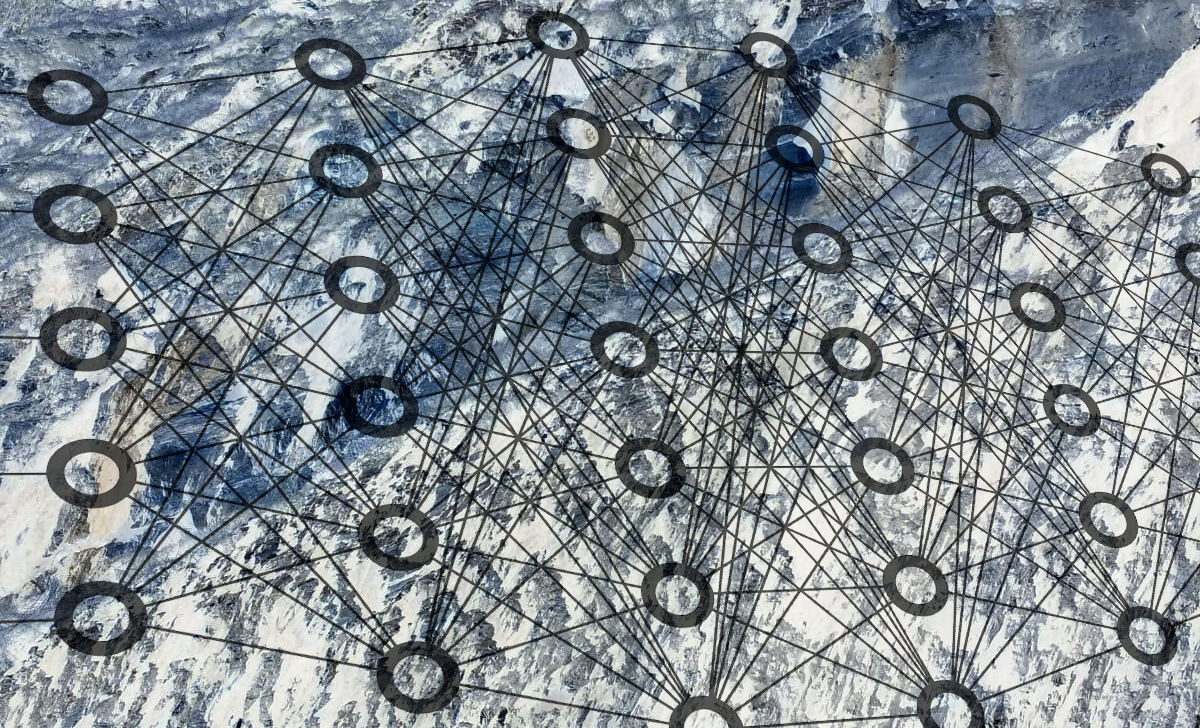
\includegraphics[height=\paperheight,width=\paperwidth]{frames/auxiliar/title_img/prueba.png}};}
%%%%%%%%
\begin{frame}[plain]

\begin{variableblock}{}{bg=myblue,fg=white}{bg=green,fg=red}
\begin{center}
\textbf{Conclusions and Future Work}
\end{center}
\end{variableblock}

\end{frame}
%%%%%%%%%%%%%%%%%%%%%%%%%%%%%%%%%%%%%%%%%%%%%%%%%%%%%%%%%%%%%%%%%%%
}
%%%%%%%%%%%%%%%%%%%%%%%%%%%%%%%%%%%%%%%%%%%%%%%%%%%%%%%%%%%%%%%%%%%
%%%%%%%%%%%%%%%%%%%%%%%%%%%%%%%%%%%%%%%%%%%%%%%%%%%%%%%%%%%%%%%%%%%
\begin{frame}{Contributions}

\begin{itemize}
\item We have employed hierarchical basis functions that effectively address the challenge of \emph{hanging nodes}.
\vspace{0.3cm}
\item We have developed \textbf{simple-to-implement} \( h \)- and \( p \)-GOA strategies that use an unconventional symmetric and positive definite bilinear form for possibly non-elliptic goal-oriented problems.
\vspace{0.3cm}
\item We have expanded upon a painless automatic \( hp \) strategy, initially developed for energy-norm adaptivity, to both non-elliptic and goal-oriented problems.
\vspace{0.3cm}
\item We have extended the applicability of a coarsening strategy to encompass parametric PDEs.
\vspace{0.3cm}
\end{itemize}

\end{frame}
%%%%%%%%%%%%%%%%%%%%%%%%%%%%%%%%%%%%%%%%%%%%%%%%%%%%%%%%%%%%%%%%%%%

%%%%%%%%%%%%%%%%%%%%%%%%%%%%%%%%%%%%%%%%%%%%%%%%%%%%%%%%%%%%%%%%%%%
%%%%%%%%%%%%%%%%%%%%%%%%%%%%%%%%%%%%%%%%%%%%%%%%%%%%%%%%%%%%%%%%%%%
\begin{frame}{Future Work}

\begin{itemize}
\item Reduce data needed to perform inversion using DL.
\vspace{0.5cm}
\item Implement adaptive integration methods in higher dimensions.
\vspace{0.5cm}
\item Develop $r$-adaptive methods to improve piecewise-polynomial approximation.
\vspace{0.5cm}
\item Solve parametric PDEs using NNs.
\end{itemize}

\end{frame}
%%%%%%%%%%%%%%%%%%%%%%%%%%%%%%%%%%%%%%%%%%%%%%%%%%%%%%%%%%%%%%%%%%%

\end{section}

\end{document}